% Copyright (C) 2014-2016 by Thomas Auzinger <thomas@auzinger.name>

\documentclass[draft,final]{vutinfth} % Remove option 'final' to obtain debug information.
\setcounter{tocdepth}{2}

% Load packages to allow in- and output of non-ASCII characters.
\usepackage{lmodern}        % Use an extension of the original Computer Modern font to minimize the use of bitmapped letters.
\usepackage[T1]{fontenc}    % Determines font encoding of the output. Font packages have to be included before this line.
\usepackage[utf8]{inputenc} % Determines encoding of the input. All input files have to use UTF8 encoding.

% Extended LaTeX functionality is enables by including packages with \usepackage{...}.
\usepackage{fixltx2e}   % Provides fixes for several errors in LaTeX2e.
\usepackage{amsmath}    % Extended typesetting of mathematical expression.
\usepackage{amssymb}    % Provides a multitude of mathematical symbols.
\usepackage{mathtools}  % Further extensions of mathematical typesetting.
\usepackage{microtype}  % Small-scale typographic enhancements.
\usepackage{enumitem}   % User control over the layout of lists (itemize, enumerate, description).
\usepackage[super]{nth}
\usepackage{multirow}   % Allows table elements to span several rows.
\usepackage{booktabs}   % Improves the typesettings of tables.
\usepackage{subcaption} % Allows the use of subfigures and enables their referencing.
\usepackage[ruled,linesnumbered,algochapter]{algorithm2e} % Enables the writing of pseudo code.
\usepackage[usenames,dvipsnames,table]{xcolor} % Allows the definition and use of colors. This package has to be included before tikz.
\usepackage{nag}       % Issues warnings when best practices in writing LaTeX documents are violated.
\usepackage{hyperref}  % Enables cross linking in the electronic document version. This package has to be included second to last.
\usepackage[acronym,toc,automake]{glossaries} % Enables the generation of glossaries and lists of acronyms. This package has to be included last.

% Define convenience functions to use the author name and the thesis title in the PDF document properties.
\newcommand{\authorname}{Eric M\"orth} % The author name without titles.
\newcommand{\thesistitle}{Interactive Reformation of Fetal Ultrasound Data to a T-Position} % The title of the thesis. The English version should be used, if it exists.

% Set PDF document properties
\hypersetup{
    pdfpagelayout   = TwoPageRight,           % How the document is shown in PDF viewers (optional).
    linkbordercolor = {Melon},                % The color of the borders of boxes around crosslinks (optional).
    pdfauthor = {\authorname},          % The author's name in the document properties (optional).
    pdftitle = {\thesistitle},         % The document's title in the document properties (optional).
    pdfsubject = {Subject},              % The document's subject in the document properties (optional).
    pdfkeywords     = {a, list, of, keywords} % The document's keywords in the document properties (optional).
}

\setsecnumdepth{subsection} % Enumerate subsections.

\nonzeroparskip             % Create space between paragraphs (optional).
\setlength{\parindent}{0pt} % Remove paragraph identation (optional).

\makeindex      % Use an optional index.
\makeglossaries % Use an optional glossary.
%\glstocfalse   % Remove the glossaries from the table of contents.

% Set persons with 4 arguments:
%  {title before name}{name}{title after name}{gender}
%  where both titles are optional (i.e. can be given as empty brackets {}).
\setauthor{Dipl.-Ing.}{\authorname}{BSc}{male}
\setadvisor{Pretitle}{Forename Surname}{Posttitle}{male}

% For bachelor and master theses:
\setfirstassistant{Pretitle}{Forename Surname}{Posttitle}{male}
\setsecondassistant{Pretitle}{Forename Surname}{Posttitle}{male}
\setthirdassistant{Pretitle}{Forename Surname}{Posttitle}{male}

% For dissertations:
\setfirstreviewer{Pretitle}{Forename Surname}{Posttitle}{male}
\setsecondreviewer{Pretitle}{Forename Surname}{Posttitle}{male}

% For dissertations at the PhD School:
\setsecondadvisor{Pretitle}{Forename Surname}{Posttitle}{male}

% Required data.
\setaddress{Pfeilgasse 43, 1080 Vienna}
\setregnumber{01325306}
\setdate{05}{03}{2019} % Set date with 3 arguments: {day}{month}{year}.
\settitle{\thesistitle}{Interactive Reformation of Fetal Ultrasound Data to a T-Position} % Sets English and German version of the title (both can be English or German).

% Select the thesis type: bachelor / master / doctor / phd-school.
% Bachelor:
%\setthesis{master}
%
% Master:
\setthesis{master}
\setmasterdegree{dipl.} % dipl. / rer.nat. / rer.soc.oec. / master
%
% Doctor:
%\setthesis{doctor}
%\setdoctordegree{rer.soc.oec.}% rer.nat. / techn. / rer.soc.oec.
%
% Doctor at the PhD School
%\setthesis{phd-school} % Deactivate non-English title pages (see below)

% For bachelor and master:
\setcurriculum{Biomedical Engineering}{Biomedical Engineering} % Sets the English and German name of the curriculum.

% For dissertations at the PhD School:
\setfirstreviewerdata{Affiliation, Country}
\setsecondreviewerdata{Affiliation, Country}

% Define convenience macros.
\newcommand{\todo}[1]{{\color{red}\textbf{TODO: {#1}}}} % Comment for the final version, to raise errors.


\begin{document}

\frontmatter % Switches to roman numbering.
% The structure of the thesis has to conform to
%  http://www.informatik.tuwien.ac.at/dekanat

\addtitlepage{naustrian} % German title page (not for dissertations at the PhD School).
\addtitlepage{english} % English title page.
\addstatementpage

\begin{danksagung*}
\todo{Ihr Text hier.}
\end{danksagung*}

\begin{acknowledgements*}
\todo{Enter your text here.}
\end{acknowledgements*}

\begin{kurzfassung}
\todo{Ihr Text hier.}
\end{kurzfassung}

\begin{abstract}
\todo{Enter your text here.}
\end{abstract}

% Select the language of the thesis, e.g., english or naustrian.
\selectlanguage{english}

% Add a table of contents (toc).
\tableofcontents % Starred version, i.e., \tableofcontents*, removes the self-entry.

% Switch to arabic numbering and start the enumeration of chapters in the table of content.
\mainmatter

\chapter{Introduction and motivation}
%!TEX root = ../main.tex
\newacronym{4d}{4D}{four dimensional}
\newacronym{3d}{3D}{three dimensional}
\newacronym{2d}{2D}{two dimensional}
\newacronym{crl}{CRL}{crown-rum length}
\newacronym{hc}{HC}{head circumference}
\newacronym{itk}{ITK}{Insight Segmentation and Registration Toolkit}
\newacronym{dicom}{DICOM}{Digital Imaging and Communications in Medicine}

Medical fetus diagnostics involves in most cases ultrasound imaging and visualization \cite{Viola2013}. The low costs and the fact that there is no radiation involved leads to a growing interest in this medical recording process and the involved visualization techniques \cite{Huang2017}. \gls{3d} ultrasound has become a major field of research since the early 1980s \cite{Correa2010}. Nowadays also \gls{4d} ultrasound imaging is possible where the \gls{3d} images are recorded in real time and represented as moving images \cite{Yagel2007}. Yagel et.al. state that \gls{3d} and \gls{4d} ultrasound scanning devices are available in many centers where fetal diagnostics is performed \cite{Yagel2007}.  The diagnostics of the fetus growth is one of the major fields where \gls{2d} and \gls{3d} as well as 4D ultrasound techniques are used \cite{Moeglin2005}. Measuring the growth of the fetal organs in addition to the overall development is a very important factor for the healthy development of the fetus \cite{Moeglin2005}. Ultrasound is widely used to measure e.g. the growth of the fetal lungs \cite{Moeglin2005}. Having a look at the general growth development of the fetus is very important for the early detection of abnormalities in development or other complications during the pregnancy \cite{Whitworth2014}.\newline\newline

Beside the organs the overall growth of the fetus is also of a great interest. Important variables are for example the \gls{crl} and the \gls{hc} \cite{Loughna2009}. There are also other measurements used to predict the fetal growth using circumferences like the head circumference or the abdominal circumference. Those circumferences are, when using 2D images not easy to describe and measure. Different approaches may be used depending on multiple measurements \cite{Loughna2009}. According to Schild et.al another interesting measurement is also the femur length because in combination wit the \gls{hc} it may be used to calculate the predicted weight of the fetus \cite{Schild2000FetalUltrasound}. Overall it can be said that measuring the fetus during the pregnancy is a very important but in some cases very tedious to perform. That is the reason why transforming the fetus to a standardized position like a T shaped position would be useful. The measurements of the limbs would be much easier and easy comparable over time. Overall height could be estimated automatically as well as the span of the arms. It can be said that a \gls{3d} visualisation and transformation as well as a guided measurement tool would be useful.

\section{Problem definition and research questions}

Transforming of given data into a specific position requires somehow knowledge of the given data in order to perform the task \cite{Singh2004}. This knowledge might be included in the dataset given or may be the result of some interaction with the user. In order to somehow anatomically correctly model a fetus into a new formation the skeleton or an abstract version of the skeleton may be used. The key points of the skeleton which have to be correctly placed in the data are the joints. The joints are the points where the different parts of the limbs rotate around in order to generate new posture of the given body. Having figured out how to incorporate the armature into the data the next step is to transform it.\newline

The transformation of the fetus has to be done in a way that the result is a fetus with his or her arms in a horizontal line and the legs shall be straight and in parallel. One may imagine the famous image of Leonardi Da Vinci named the vitruvian man where a man is drawn in a perfect T-position. Figure \ref{fig:vitruvianMan} shows the famous picture. The problem at this step is to find out how the different parts have to be transformed in order to bring them into that special shape. 

\begin{figure} [!htb]
    \centering
	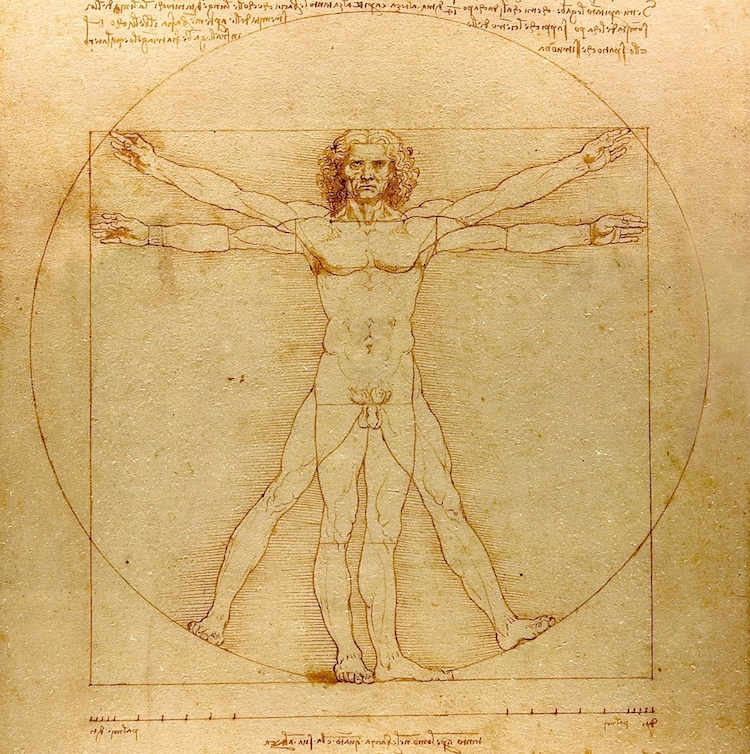
\includegraphics[width=10cm]{content/images/vetruvianMan.png}
	\caption{The vitruvian man by Leonardo da Vinci \cite{daVinci1492TheMan}.} 
	\label{fig:vitruvianMan}
\end{figure}

\section{Overview of the aimed solution}
Having a look at the clinical procedure when performing fetus analysis there is definitely a room for improvement. The first step is to acquire the data of the fetus. This step may be one of the most important ones because it determines the completeness and the quality of the fetal data. Therefore this step should already be guided and in a way that the clinical personal is able to perceive the data which is already acquired and where some additional data may be useful. In order to be able to capture and visualize a fetus during the ultrasound session the compounding feature introduced by Viola et. al. may be of a great interest \cite{Viola2013}.\newline

After the recording of the data the processing of it is the next step. The idea is that the fetus is processed in a way that it can be presented in a T-position. This position enables different kinds of measurements and enables a clear view of the limbs as well as the head. At some point one might consider the interaction with the operator of the program useful and fruitful and this might be one of those. The process of interactively reforming the fetus data into a given position requires first the integration of a so called armature into the data. The armature describes the joints and bones of the skeleton in an abstract way. Some points may be moved into the data automatically but it might be a better solution to ask the operator of the system to define some key points and let the machine describe the rest of the data.\newline

After having the armature embedded in the data the weighting has to be done. Weighting means that the program has to calculate the affinity of voxels to segments of the armature. This step can be done completely automatically. After the volume data has been linked to the armature the transformation can be done. The transformation analyses the position of the armature and moves each part of the limbs of the fetus against others in respect to the joints. The angles which have to be used when applying the rotations in 3D space may be calculated and applied automatically. The result should be a representation of the acquired fetus data showing the whole fetus at a glance in a T-position.\newline

The end results may also include the standardized measurements automatically taken by the machine. The introduction of this system may also lead to the development of new measurements which take the whole span from finger to finger or the size of the fetus from head to toe. The representation of a fetus in a standardized way also enables the data to be comparable in means of time or inter specimen differences.

\section{Requirements}

Loading the volumetric data of the fetal ultrasound analysis into the program shall be rather easy and the system should support well-known file formats used in medicine like the file formats used by the \gls{itk}. Another approach would be to use the file format called \gls{dicom} which is commonly used in clinical application or generally when working with medical data.\newline

If the source is an ultrasound investigation preprocessing to remove artefacts might be applied. The processing may include filtering to get rid of artefacts induced by for example the mother fluid or interactions with the tissue which the sound wave has to cross in order to perceive the fetus. In ultrasound images the data which represent the fetus normally have a specific range of values, therefore a threshold may be applied. If the further processing steps also assume or require that the data only includes the fetus and nothing else a largest connected component analysis should also be performed. This step searches, like the name says the largest connected component in a \gls{3d} volumetric dataset which should be the fetus. The rest of the image may be declared as artefacts or not relevant and can be neglected.\newline

The solution shall provide an interface where the user is able to interact with the system. The system shall provide an "easy to use" graphical desktop where the interaction is carried out. A  pipeline that guides thought the different steps of the transformation would be appreciated. In general the aim is to minimize the input needed from the end-user and shift the focus on automatic processing of the data. One step where interaction is very likely to be used is the rigging of the data. Finding a skeleton or incorporating a predefined armature into the data may be out of scope of this thesis and therefore user interaction is thinkable. The integration of the armature into the data should not take too much time and has to be very easy to carry out. The armature or skeleton is a preset where all the joints and the bones are already defined and only have to be put at the right spot inside of the volume. This step can be done by using a simple drag and drop interaction in a \gls{3d} view of the model. The user therefore has to be somehow familiar with the navigation in volume explorer and should have some kind of anatomical knowledge.\newline

Once the armature is at the right spot the weighting of the voxels has to be performed. This step is also called skinning, because the data is attached to the armature like a skin. This step should also work automatically but user interaction may be included in order to review and check the assignment. The assignment of the data to specific bones may be overwritten by the operator in order to deliver better results. The program should evaluate and preferably also visualize the belongingness of the voxels to the armature parts.\newline

The main step of the processing steps introduced in this thesis namely the T-transformation should be performed completely automatically and the results should also be exportable for further visualization and analysis. Transforming the data should not require any further input or interaction with the user. The data and the armature should be the only input for the module handling the transforming process. The end result although should again be inspectable and there should be some possibilities to automatically measure the fetus. It can also be thought of automatically display the main measurements like the span from fingertip to fingertip and from head to toe.  

\newpage

\chapter{Clinical background}
\newacronym{mri}{MRI}{magnet resonance imaging}
\newacronym{vocal}{VOCAL}{Virtual Organ Computer-aided Analysis}

In this section the clinical background of the data and the processing steps is verbalized. The source of the data and the different forms of data acquisition are especially important in order to understand why different processing steps have to be performed. Linking the visualization and the processing of the medical data to their origin and thinking about possible applications is also important for understanding the overall concept.

\section{Related data and data acquisition}

According to Huang and Zeng \cite{Huang2017} real-time \gls{3d} ultrasound imaging is a very well accepted technique in medicine, because it provides interactive feedback for the clinicians. Violea et. al. state that there are different issues when working with ultrasound data like noise or other visual artefacts \cite{Viola2013}. It is very important to have a precise navigation and visual feedback in order to acquire meaningful data with a high level of details \cite{Viola2013}. One problem in 3D ultrasound is that the perceivable volume might not be large enough to record the whole range of interest. This problem occurs in many cases for example when examining inner organs like the liver but it is also a very prominent issue when working with fetal data \cite{Viola2013, Lee1995ThreeMode}.\newline

The data delivered by 3D ultrasound can be seen as a cloud of data points aligned at a \gls{3d} grid. In case of a fetal examination they can represent various things like mother fluid, artefacts from the tissues which the signal of the ultrasound has to travel through or also organic tissue which is floating in the mother fluid as well as of course the fetus. The data points have to be characterized and it has to be clear which of them really belong to the fetus, obviously the object of interest. Having a look at the anatomy of the woman the data acquisition may be somehow tricky. The belly is very well exposed and it leads to beautiful pictures from one side but having a look at the other side of the fetus may be impossible. The ultrasound waves do not travel very well through hard tissue like bones and therefore the examination of the fetus through the back of a woman is not helpful. A schematic explanation how a fetal ultrasound investigation is carried out is depicted in Figure \ref{Fetal_Ultrasound}.\newline\newline

\begin{figure} [htb!]
    \centering
	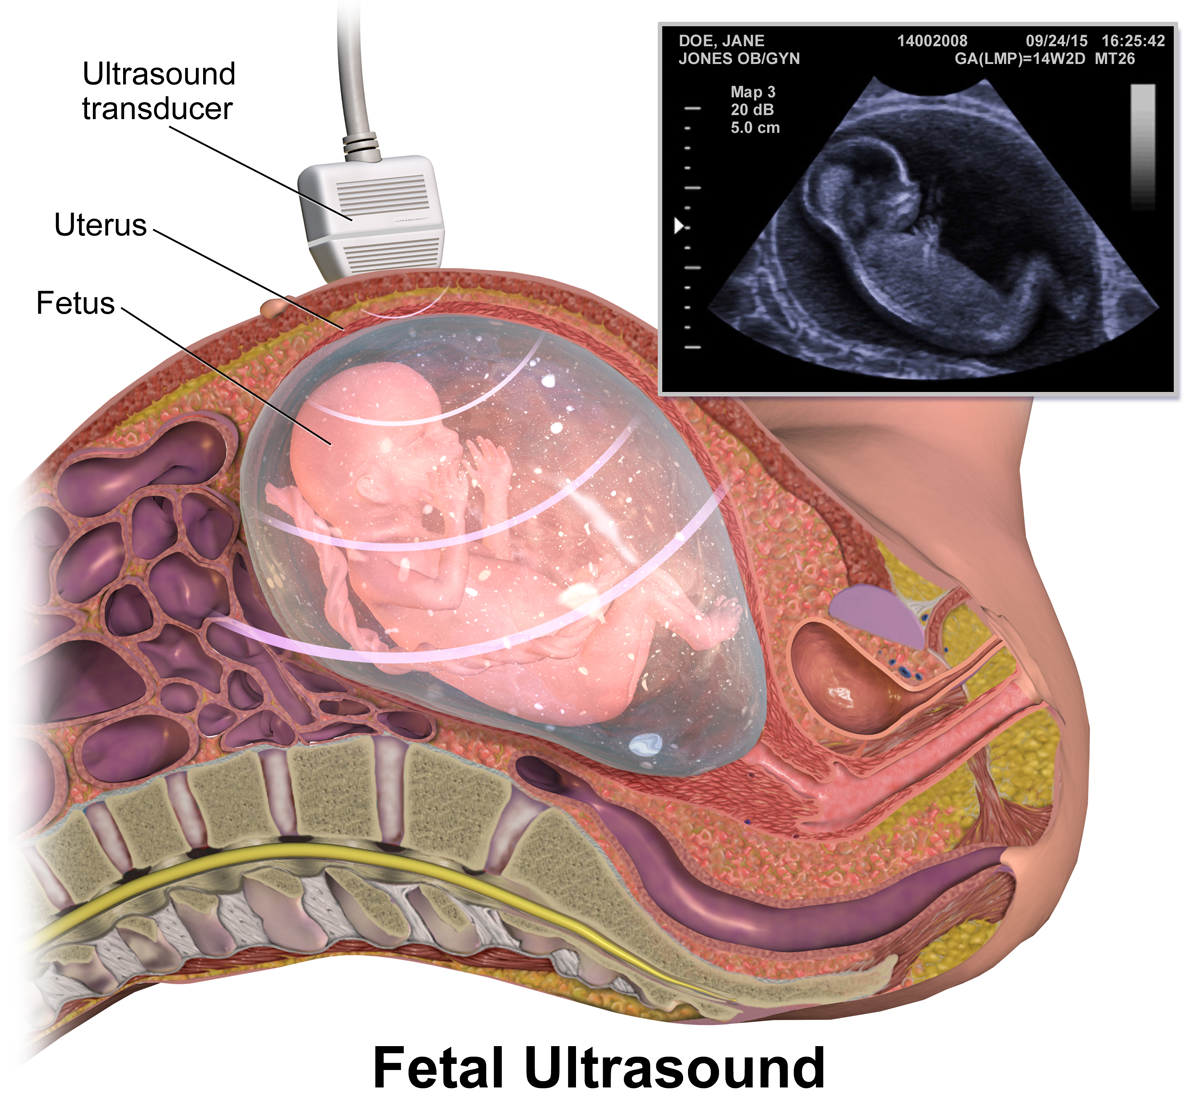
\includegraphics[width=12cm]{content/images/Fetal_Ultrasound}
	\caption{Schematic description of how a fetal ultrasound investigation is carried out including anatomical details of the pregnant woman \cite{BruceBlausFetalUltrasound}.}
	\label{Fetal_Ultrasound}
\end{figure}

\section{Analysis of the data}
\gls{2d}, \gls{3d} and also \gls{4d} ultrasound investigations are techniques which are without a doubt very important for the analysis of a fetus. Gathering insight of the fetal surface as well as the organs and the cardiovascular system are essential for supporting a healthy development.

\subsection{Organ analysis}

The development of the inner organs is a very important aspect in the early development of a human being. Many problems during the growth phase of the essential organs like the heart or the lungs are induce from the outside. Therefore in case of growth issues expectant mothers could be advised on how to avoid bad influences.

\subsubsection{Lung growth}

Moeglin et. al. state that various ultrasound techniques may be used to identify fetal lung growth \cite{Moeglin2005}. They write about using \gls{2d} and \gls{3d} ultrasound based approaches as well as \gls{mri} based techniques. The \gls{mri} based measurements are able to encounter more detailed analysis because they able to overcome the limitations of ultrasound based imaging but the downside is that the costs are higher, the patient compliance is lower and it is highly affected by the fetal movement \cite{Moeglin2005,Bonet-Carne2015QuantitativeMorbidity}.\newline\newline
Fetal lung volume might be measured using the \gls{vocal} software by General Electric Medical Systems KretzTechnik which is able to produce a \gls{3d} model of the lung. A representation of the graphical output of the software can be seen in Figure \ref{fig:fetal_lung_volumetry} \cite{Moeglin2005}.\newline

\begin{figure} [htb!]
    \centering
	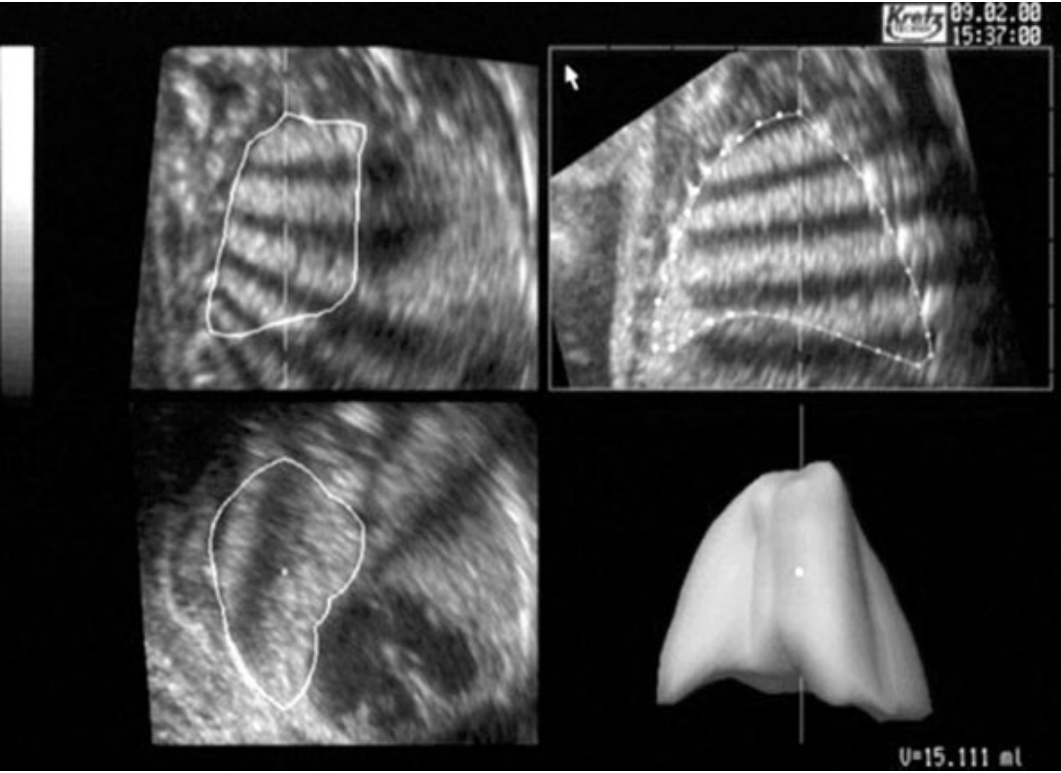
\includegraphics[width=12cm]{content/images/fetal_lung_volumetry}
	\caption{Output of the \gls{vocal} software using an rotation technique to estimate the fetal lung volumetry. The lung volume is estimated by rotating it around the vertical axis. In the lower right corner a produced 3D model of the lung can be seen \cite{Moeglin2005}.}
	\label{fig:fetal_lung_volumetry}
\end{figure}
\newpage
\subsubsection{Cardiovascular system}

The fetal cardiovascular system is also subject of analysis \cite{Yagel2007,Baschat2011ExaminationSystem,Dong2013PreliminaryAnomalies}. It suffers from congenital pathology most often \cite{Dong2013PreliminaryAnomalies}. \gls{3d} ultrasound and modern visualization techniques can for example be used in order to examine and visualize the inter ventricular septum \cite{Yagel2007}. Figure \ref{fig:septum} represents the ultrasound image and the surface rendering of the septum.

\begin{figure} [htb!]
    \centering
	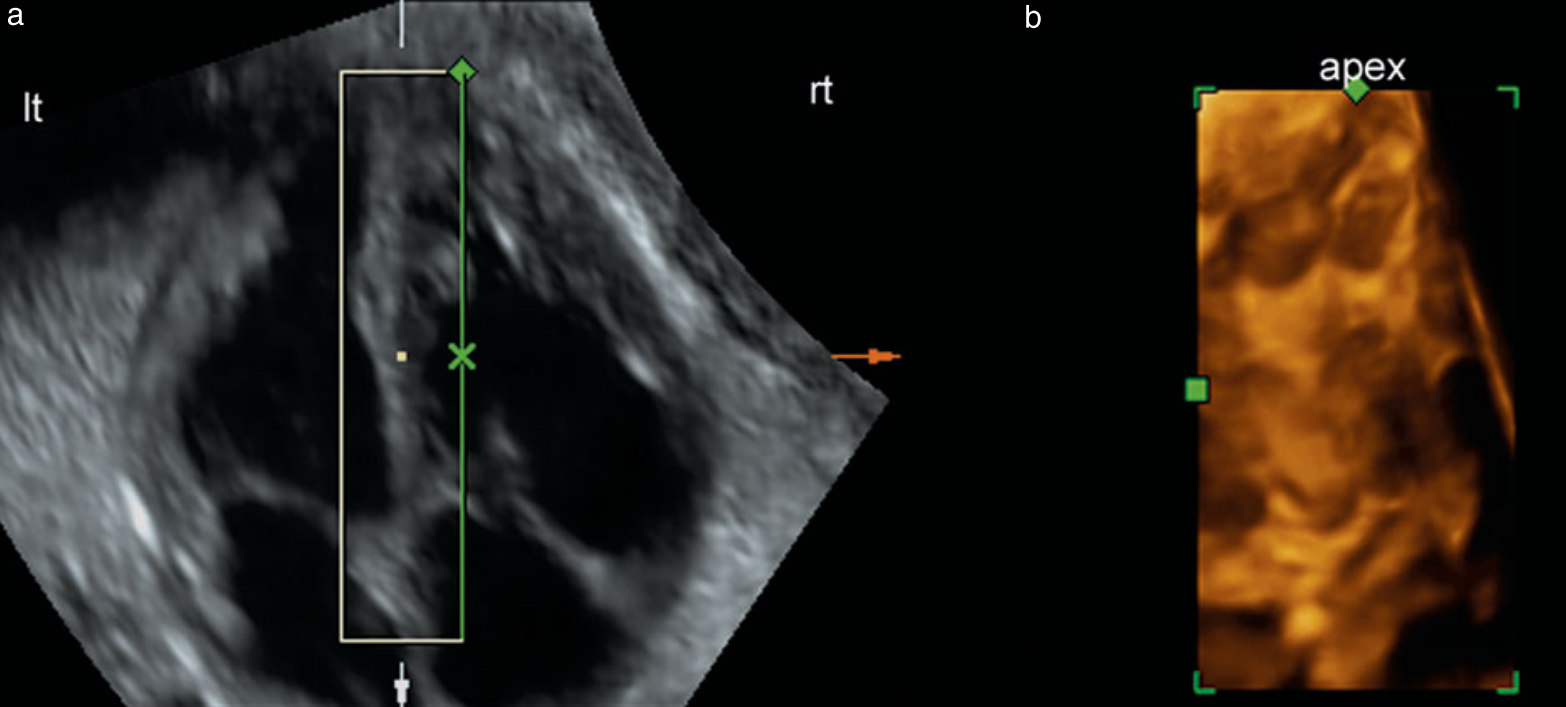
\includegraphics[width=13cm]{content/images/septum}
	\caption{Left left side of the image shows the ultrasound image of the heart and the interventricular septum is inside of the green box. The surface of the septum is visualized on the right side which might help doctors to examine for abnormalities \cite{Yagel2007}.}
	\label{fig:septum}
\end{figure}

Another important measurement at the cardiovascular level is to measure the cardiac output volume using Doppler evaluation \cite{Baschat2011ExaminationSystem}. Baschat shows in his paper that this technique may be used to examine the flow through different vessels in a fetus in order to find out if there is any occlusion or abnormality \cite{Baschat2011ExaminationSystem}. The author states that it is an essential tool for perinatal specialists for the generation of clinical diagnoses. Figure \ref{fig:cardioPulmonary} shows an example of how the output of such a Doppler evaluation may look like.

\begin{figure} [htb!]
    \centering
	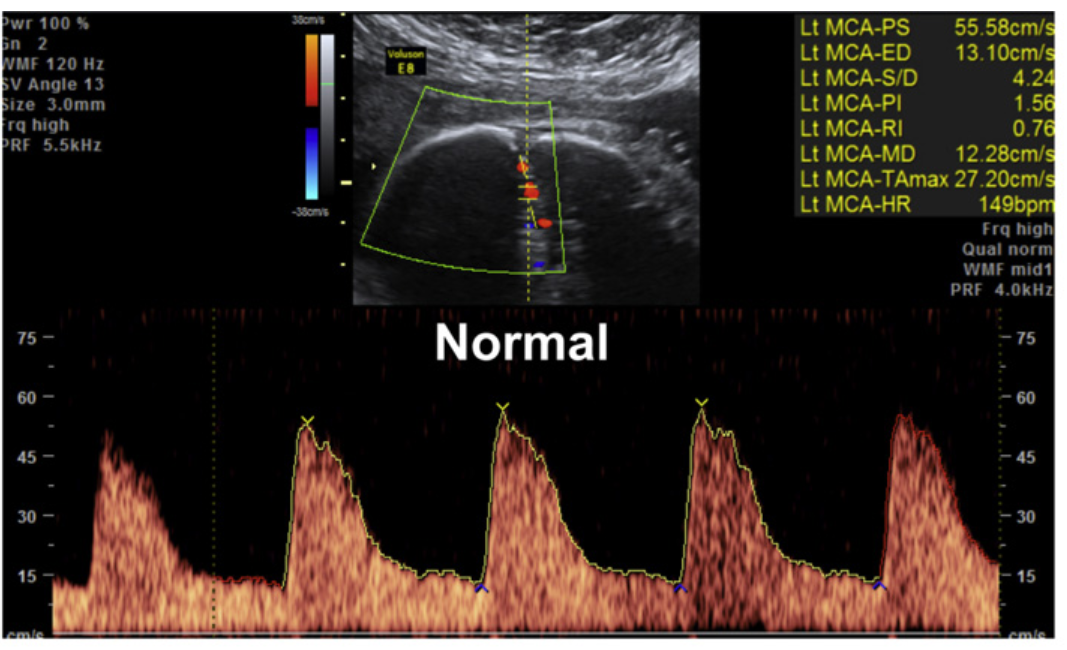
\includegraphics[width=13cm]{content/images/cardioPulmonary}
	\caption{Doppler signal of the middle cerebral artery of a fetus \cite{Baschat2011ExaminationSystem}.}
https://www.overleaf.com/project/5c7edf5a9c804c4085911acb	\label{fig:cardioPulmonary}
\end{figure}

\newpage
\subsection{Facial development}

Another very important aspect which can be examined using \gls{3d} ultrasound is the development of the face of the fetus. The information about facial deformations is not only important for obstetricians or paediatricians the surface visualization of the given data is also important when telling the parents \cite{Lee1995ThreeMode}. It can be somehow tough to explain them with words that their child is going to have deformations in the face but showing them makes it a lot easier to perceive. An example for such a facial surface visualization is depicted in Figure \ref{fig:face}.

\begin{figure} [htb!]
    \centering
	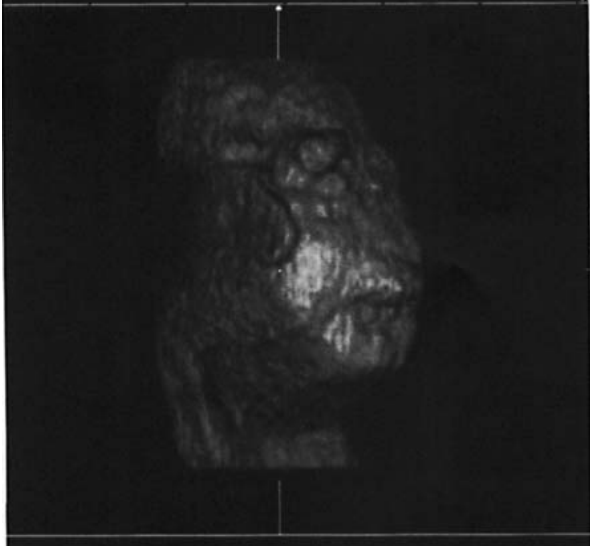
\includegraphics[width=10cm]{content/images/face}
	\caption{Ultrasound surface visualization of a male fetus in the \nth{30} week of pregnancy. The face does not show any regular facial structure \cite{Lee1995ThreeMode}.}
	\label{fig:face}
\end{figure}

\subsection{Fetal growth analysis}\label{subsct:fetalGrowth}

Fetal size measurement more general growth analysis is a well known topic and many different scientists have written about it \cite{Hadlock1984EstimatingParameters.,Schild2000FetalUltrasound,Loughna2009,Whitworth2014}.The size and the weight of the fetus is of a special interest for the clinicians in the birth preparation. Knowing what to expect can be very important during the birth. In earlier times the growth analysis has only taken the \gls{2d} images into account and the measurements where for example the following: \gls{crl} or \gls{hc}. Those are very well defined and Loughna et. al. perfectly illustrate how to measure them which may be seen in Figure \ref{fig:crlmeasurement} and Figure \ref{fig:hc} \cite{Loughna2009}. The head circumference is measured using the outer to outer biparietal diameter and the occipital-frontal diameter \cite{Loughna2009}.

\begin{figure}[htb!]
    \begin{minipage}{7cm}
        \centering
        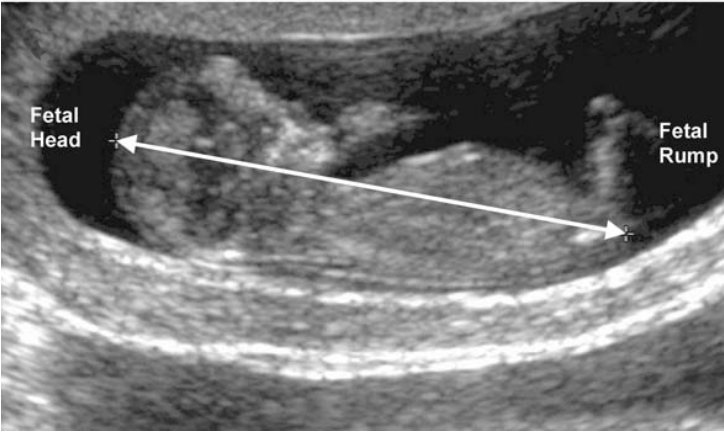
\includegraphics[width=7cm]{content/images/crlmeasurement}
        \caption{Crown-rump measurement of a fetus \cite{Loughna2009}.}
        \label{fig:crlmeasurement}
    \end{minipage}
    \hspace{0.02\textwidth}
    \begin{minipage}{7cm}
        \centering
        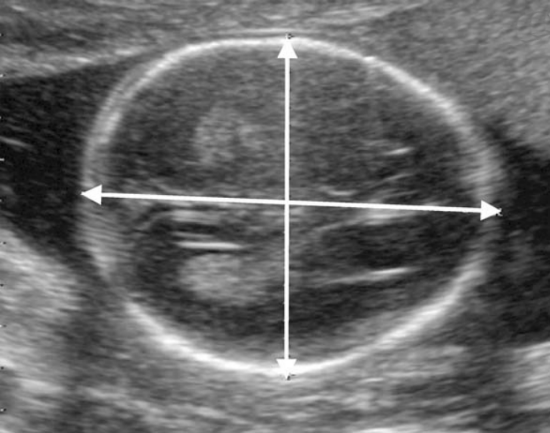
\includegraphics[width=5.35cm]{content/images/hc}
         \caption{Head circumference measurement  \cite{Loughna2009}.}
         \label{fig:hc}
    \end{minipage}
\end{figure}

\newpage
Another important measurement is the femur length. Hadlock et.al. state that the head circumference in combination with the femur length are a strong predictor of the fetal age \cite{Hadlock1984EstimatingParameters.} Knowledge about the age is essential in the fetal growth analysis because only with this information the growth is comparable to standardized tables like stated in \cite{Loughna2009}.\newline\newline

\gls{3d} ultrasound also plays a role in fetal growth analysis. Schild et.al. found out that using the three dimensional data produced by the \gls{3d} ultrasound, weight estimation can be enhanced \cite{Schild2000FetalUltrasound}. They also use the influence of soft tissue in order to find out more about the constitution of the fetus and the effects of this on the weight \cite{Schild2000FetalUltrasound}. \newline

The growth analysis is done over the whole pregnancy of the woman starting with the \nth{13} week and ending with the \nth{42} \cite{Loughna2009}. In this period of time the growth is calculated using the formulas presented in the paper of Loughna et.al. and than compared with standardized tables \cite{Loughna2009}. The problem which may arise here is that those measurements take some time and have to be performed for every investigation. A standardized position or pose of the fetus may be helpful to not only visualize the growth of the fetus in the different stages of the pregnancy but also analytically calculate it.  


\newpage

\chapter{Related work}\label{ch:related}
\newacronym{gpu}{GPU}{graphics processing unit}
\newacronym{ik}{IK}{inverse-kinematics}
\newacronym{lbs}{LBS}{linear blend skinning}
\newacronym{ct}{CT}{computed tomography}

In this section the related works will be announced and summarized. The section is segmented topic wise and it also includes previous works of ideas that may not have managed to be implemented in the course of this thesis.

\section{Ultrasound data handling}

From a technical perspective ultrasound is an acoustical investigation and therefore is susceptible of various noise induced artefacts \cite{Solteszova2012}. The ultrasound investigation is somehow limited to the investigation area which is unable to perceive for example the whole liver or also the whole fetus at a glance \cite{Viola2013}. Therefore techniques to generate compund volumes on the fly are important \cite{Viola2013,Muller2014}. 

\subsection{Filtering 3D ultrasound}

Especially when using \gls{3d} ultrasound investigations in a medical context some kind of filtering is essential in order to perceive anatomical structures visually and mentally. Therefore Solteszova et.al. introduced a technique called Lowest-Variance Streamlines for filtering \gls{3d} ultrasound \cite{Solteszova2012}. The filtering identifies borders of structures by calculating the lowest variance direction. According to Solteszova et.al. their procedure is similar to a streamline integration in a vector field. The approach is interesting because it is especially useful for medical ultrasound applications in order to reduce artefacts like noisiness and speckles which may lead to a miss interpretation of the underlying data. The output of the filtering method can be seen in Figure \ref{fig:Streamline}.

\begin{figure} [htb!]
    \centering
	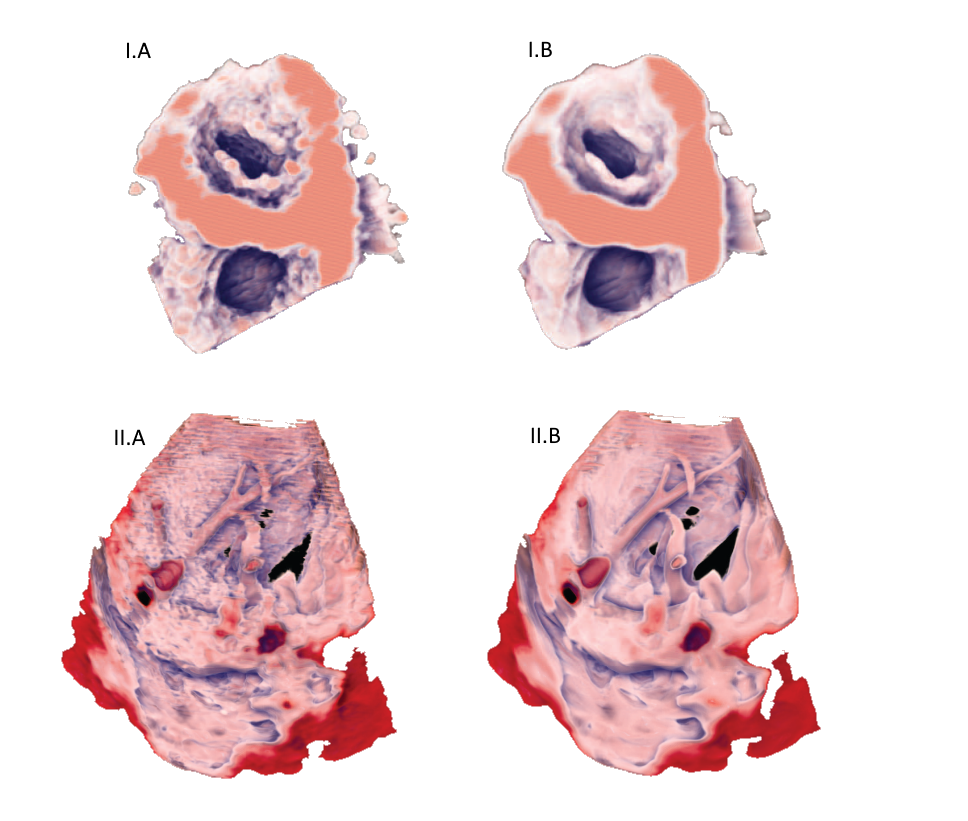
\includegraphics[width=16cm]{content/images/streamline}
	\caption{I.A and I.B depict a cardiac ultrasound before and after filtering and II.A and II.B show an ultrasound of the liver before and after filtering \cite{Solteszova2012}.}
	\label{fig:Streamline}
\end{figure}

\newpage
Solteszova et.al. also introduced another approach for filtering especially fetal ultrasound called the output-sensitive filtering of streaming volume data \cite{Solteszova2017}. The approach is espaccially design to be used in \gls{4d} ultrasound investigations where it is important that the filtering is very fast and accurate. They limit the filtering to regions of the volume which have a potential to have an effect on the image e.g. occluded regions don't have to be filtered because they cannot be seen anyways. They state that their approach is an important improvement for streaming volume data as it is the case in a \gls{4d} ultrasound investigation. The output of the filtering applied to a fetal ultrasound investigation of Anna is depicted in Figure \ref{fig:outputSensitive}.

\begin{figure} [htb!]
    \centering
	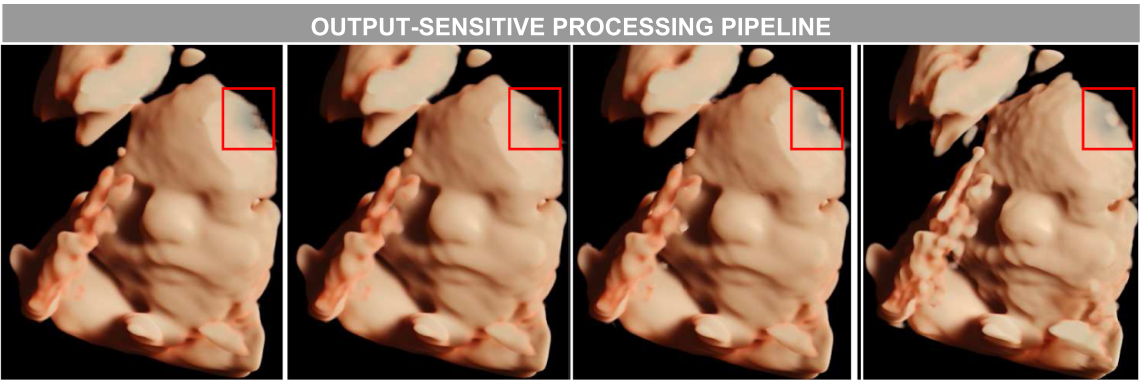
\includegraphics[width=16cm]{content/images/outputSensitive}
	\caption{The output of the otput-sensitive processing pipeline with different percentage amounts of voxels filtered. From 38\% on the left side to 0\% on the right side \cite{Solteszova2017}.}
	\label{fig:outputSensitive}
\end{figure}

\newpage
\subsection{Compound volume generation}

Viola et.al. states that a compound view of volumetric data created by ultrasound investigation can be useful for clinical investigation \cite{Viola2013}. It enables the clinicians to e.g. slice through an whole organ after is has been registered at a glance. Especially in fetal ultrasound investigation after a specific time, when the fetus is too large to be perceived as a whole, registering the data as well as producing a compound-volume is very useful and essentially for the introduced procedure. The possibility to swipe with the ultrasound investigation probe over the body and seeing the result on the screen in real-time producing a compound volume is essential for a better understanding of the examined specimen. The creation of a compound volume presented by Viola et.al. is depicted in Figure \ref{fig:SwipeVol}.

\begin{figure} [htb!]
    \centering
	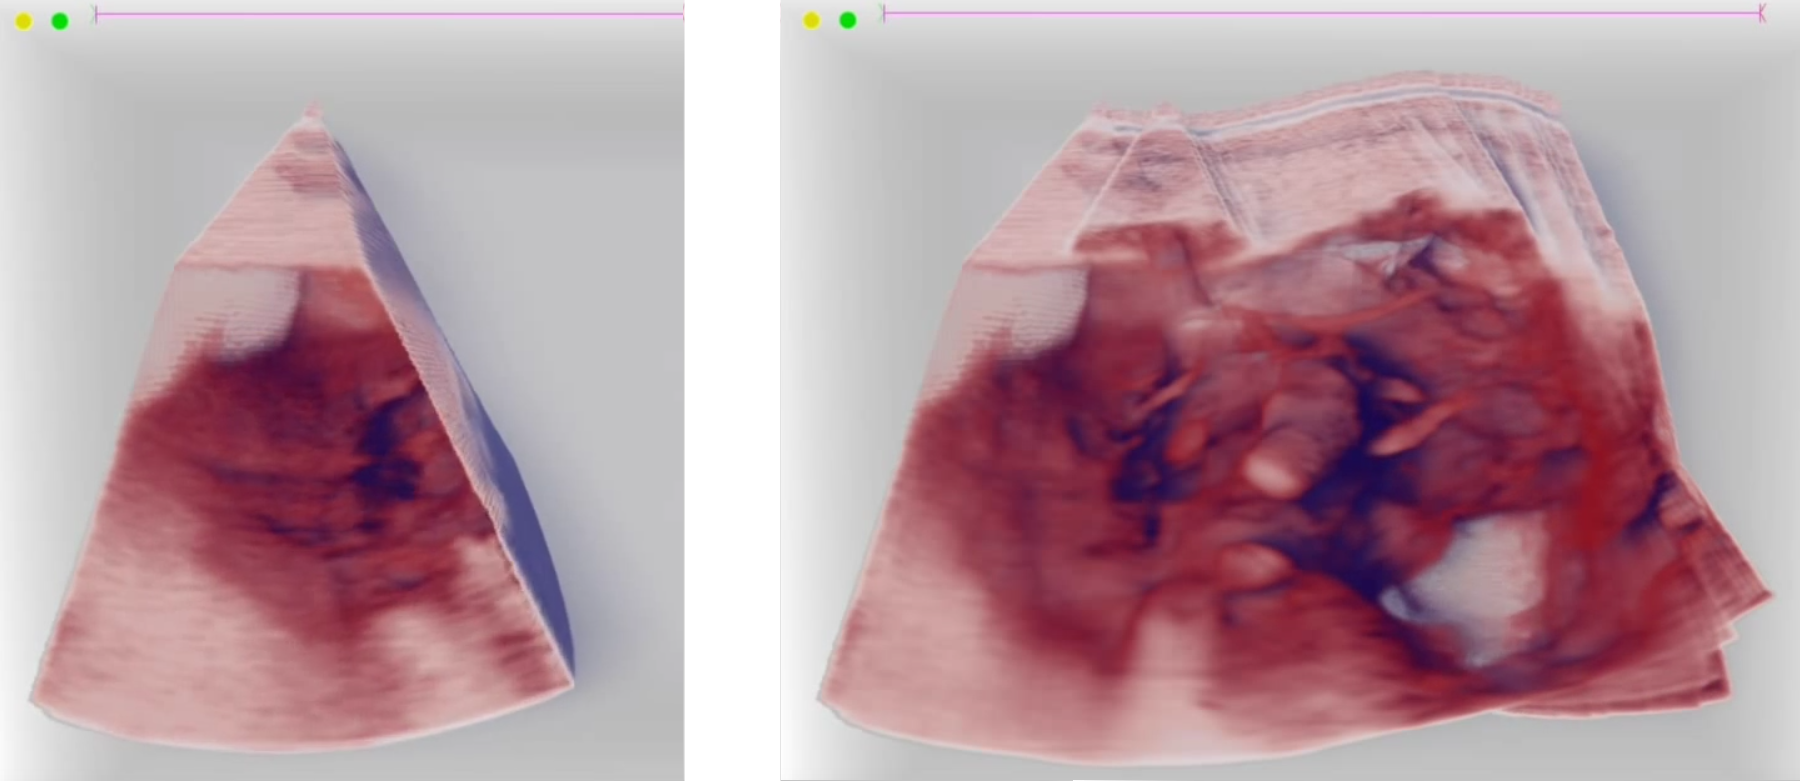
\includegraphics[width=12cm]{content/images/Swipevol}
	\caption{On the fly creation of a compound volume by Viola et.al. The right part of the image in comparison to the left part shows the progress of the compound volume generation. The images have been taken from the video of \cite{Viola2013}.}
	\label{fig:SwipeVol}
\end{figure}

Being able to automatically register and process \gls{4d} ultrasound data without externally tracking the ultrasound probe can be tough \cite{Muller2014}. Mueller et.al. state that their approach of generating a compound volume of the liver uses multi-modal registration considering the \gls{3d} voxel neighbourhood. They have used various transformations and optimization strategies in order to register the different ultrasound investigations during one session. They also had to cope with anatomical distortions of the ultrasound investigation which they stated had not an significant impact if the continuous motion of the investigation sweep had no rapid changes in direction.\newline\newline

\section{Understanding the data}
Having the ultrasound data of the fetal investigation filtered and registered in order to generate the whole volume the next steps will be about figuring out the position of the fetus. There are different approaches to find more detailed content wise information of volumetric data. One step would be to skeletonize the data and try to find out if the joints and bones of the fetus can be found automatically \cite{Singh2004,Jin2017,Jalba2013}. Another approach is to rig the data by include a predefined armature or skeleton which is than either automatically \cite{Baran2007,Baran} or manually \cite{Finet2014Bender:Morphing} included in the data. 

\subsection{Skeletonization}

Skeletonization of data is an approach where it is tried to reduce the given object to the most important features \cite{Singh2004}. This description may then be used for further processing and can be linked back to the data it has been abstracted from \cite{Jalba2013}. When writing about \gls{3d} skeletonization one has to distinguish between surface and curve skeletons. According to Jalba et.al. the surface skeleton of a \gls{3d} shape is the collection which contains the "loci of maximally-inscribed balls in a shape" \cite{Jalba2013, Pizer2003MultiscaleProperties}. In respect to the surface skeleton the curve skeleton may be described as one dimensional curves which are positioned at the center of the \gls{3d} shape. The second skeleton is especially interesting when trying to transform fetus data. Jalba et.al. presented a technique which is based on the \gls{gpu} for calculating curve skeleton points by firstly evaluating the surface skeleton and then detecting the curve skeleton points by their algorithm \cite{Jalba2013}. Their algorithm works fast and reliable and delivers a high-quality curve skeleton and automatically delivers the mapping to the underlying data. The results of their approach are depicted in Figure \ref{fig:CurveSkeleton}.

\begin{figure} [htb!]
    \centering
	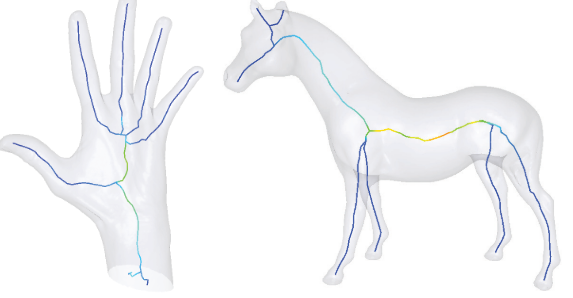
\includegraphics[width=11cm]{content/images/curveSkeletonJalba}
	\caption{Result of the curve skeleton produced by the algorithm introduced by Jalba et. al. for a human hand on the left and a horse on the right \cite{Jalba2013}.}
	\label{fig:CurveSkeleton}
\end{figure}

\newpage
Another approach to produce a skeletal representation of in that case voxel data is presented by Jin and Kim \cite{Jin2017}. Their algorithm is based on a thinning approach and can be implemented on the \gls{gpu}. Jin and Kim identified general patterns of \gls{3d} neighbourhood relation which can be used in order to decide if a voxel is part of the skeleton or not. The algorithm can be executed in parallel for each voxel in the data. They also introduced a skeleton correction algorithm which takes care of connecting skeletal parts which may have been disconnected by the thinning algorithm. The authors evaluated their approach using 100 models of the SHREC 2015 benchmark testing set and state that their proposed algorithm is robust and provides an overall good performance. The results when performing on a human model can be seen in Figure \ref{fig:skeletonThinning}.

\begin{figure} [htb!]
    \centering
	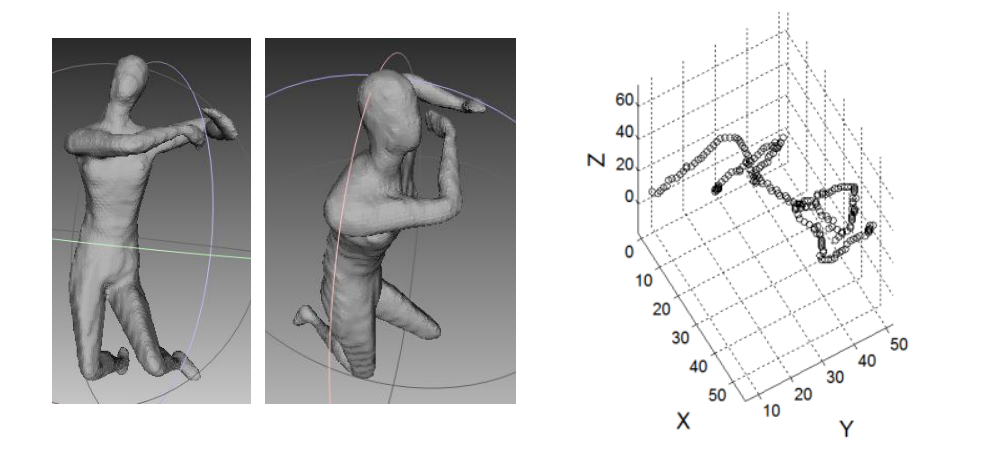
\includegraphics[width=14cm]{content/images/skeletonThinning}
	\caption{Human model and the skeletal representation using the partial parallel \gls{3d} thinning based skeletonizaion algorithm introduced by Jin and Kim \cite{Jin2017}.}
	\label{fig:skeletonThinning}
\end{figure}

A third approach of gathering the skeleton of a \gls{3d} model is presented by Singh and Silver \cite{Singh2004}. They used two approaches one is based on the calculation of the curve skeleton introduced by Gagvani \cite{Gagvani1999} and the other one is based on a potential field algorithm shown by Cornea et.al. \cite{Cornea2005ComputingObjects}. Singh and Silver state that they use both approaches in order to get the \gls{ik} skeleton of the data which does not only consist of the simple skeleton but also has information about bones and joints \cite{Singh2004}. This information is especially important when thinking of interactively transforming data to another position. The positioning of the joints and the bones on the skeleton can be performed manually or semi-automatically. The semi-automatically approach uses the potential field algorithm and the manually one the thinning algorithm. The authors state that the semi-automatically way may be more user-friendly on the other hand the algorithm used in the manual processing is faster \cite{Singh2004}. One major benefit of the algorithm introduced by the authors is that they already automatically calculate the correspondence of each voxel to the specific bone. This is also a huge benefit when thinking of transforming data to a new position. Figure \ref{fig:ikskeleton} represents the data and the corresponding \gls{ik} skeleton.

\begin{figure} [htb!]
    \centering
	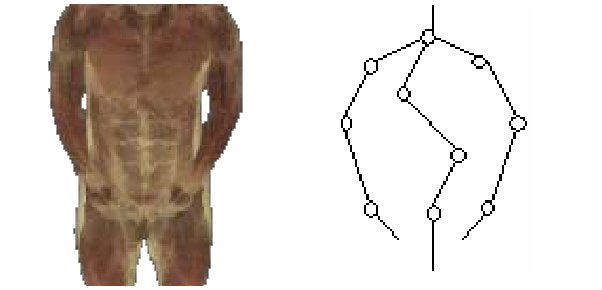
\includegraphics[width=12cm]{content/images/ikskeleton}
	\caption{The given data and the corresponding \gls{ik} skeleton can are figured. The skeleton already features the joints where parts of the volume can be move against \cite{Singh2004}.}
	\label{fig:ikskeleton}
\end{figure}
\newpage

\subsection{Rigging approaches}

Rigging defines the process to determine the skeletal structure and the position of it in a \gls{3d} model in order to be able to move parts of the model and knowing how the surface or the volume has to be deformed \cite{Baran2007}. This task can either be performed in a manually way needing an animator or similar professional to define the skeleton and the position or in an semi-automatic or automatic way. The complexity to automatically rig a \gls{3d} model should not be neglected.

\subsubsection{Pinocchio}
The first approach for automatically rigging a \gls{3d} model represented by its mesh is introduced by Baran and Popovic \cite{Baran2007}. The procedure creates a distance field from the given mesh and it identifies a skeleton by approximating the medial surface. The extracted skeleton is than fitted to template skeleton to refine the output. For their approach they are using discrete penalty functions in order to match the extracted skeleton to a pre defined so called instruction how a skeleton should look like. For example the penalty function checks where the feet are and that they should be on the ground and not at the top area of the mesh. With those penalty functions it can clearly be seen that the method looses generality. The general approach of rigging in the Pinocchio prototype is shown in Figure \ref{fig:pinocchio}.

\begin{figure} [htb!]
    \centering
	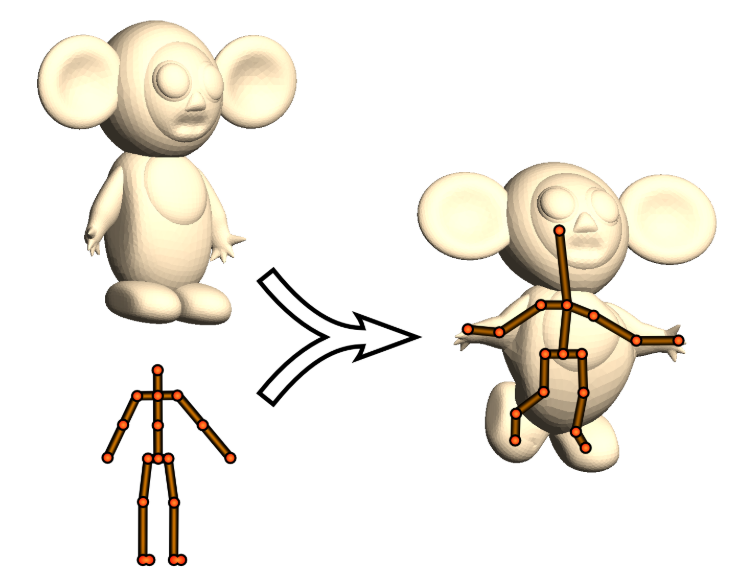
\includegraphics[width=11cm]{content/images/pinocchio}
	\caption{General overview of the pinocchio rigging prototype placing an predefined skeleton into a \gls{3d} mesh model by extracting the curve skeleton and than matching it with a pre-defined prototype skeleton \cite{Baran2007}.}
	\label{fig:pinocchio}
\end{figure}

\newpage
Shapiro et.al. introduce another approach which is quite similar to the strategy of Baran and Popovic but uses voxels instead of the mesh representation of the \gls{3d} model \cite{Shapiro2014RapidSensors}. They have tried to make \gls{3d} scans of humans available for using them in computer animations. Therefore they scanned the humans in four different poses and created a \gls{3d} model out of the gathered data. The difficulty of the rigging was that their mashes where not perfect and had holes and other artefacts. Therefore they decided to create a voxelized version of the mesh by using depth buffer carving. The data they use are produced by the consumer product Kinect \cite{Shapiro2014RapidSensors}. After voxalizing the data they used the same technique as Baran and Popovic \cite{Baran2007} to find the skeleton in the mesh. The approach therefore has the same downside that it does not allow the model to be in another formation before the rigging is done. It has to be in a predefined initial position. The output of the procedure is depicted in Figure \ref{fig:saphiro}.

\begin{figure} [htb!]
    \centering
	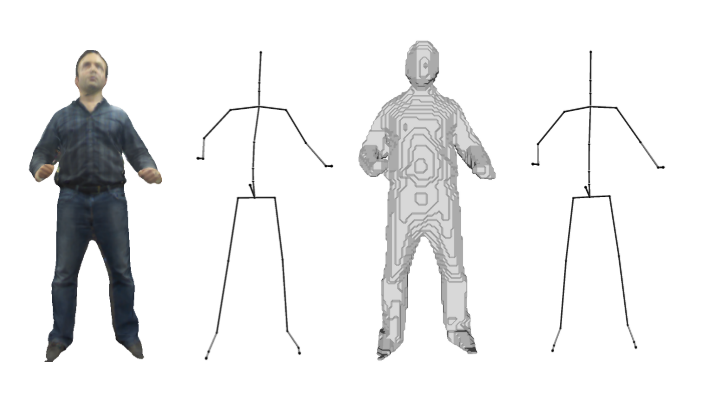
\includegraphics[width=13cm]{content/images/saphiro}
	\caption{On the left the original mesh of the human \gls{3d} scan and the corresponding skeleton. On the right the voxel representation of the mesh using the depth buffers and the skeleton of it. It can be seen that the skeletal representation looks the same for both representations of the \gls{3d} model \cite{Shapiro2014RapidSensors}.} 
	\label{fig:saphiro}
\end{figure}

\subsubsection{Joint mapping}

Bharaj et.al. introduce a procedure which is able to automatically rig a character by using a joint mapping technique \cite{Bharaj2012}. Their approach is especially suitable for multi component characters. They are using point clouds in order to sample each identified component of the input model. These clouds are represented as a a graph which is simplified and transformed into a tree by using clustering. Their attempt needs as a second input an animation skeleton which is predefined. The authors use joint mapping in order to find the relation between their tree and the given animation skeleton. Normally the mapping is defined by a user. Their approach is closely related to the approach stated in this thesis because they also would like to afterwards find a way to transform the data into a standardized T-pose \cite{Bharaj2012}. The transformation of the data can be done using an animation software because their export format is an industrial standard. Two examples of their rigging process can be seen having a look at Figure \ref{fig:bharaj}.

\begin{figure} [htb!]
    \centering
	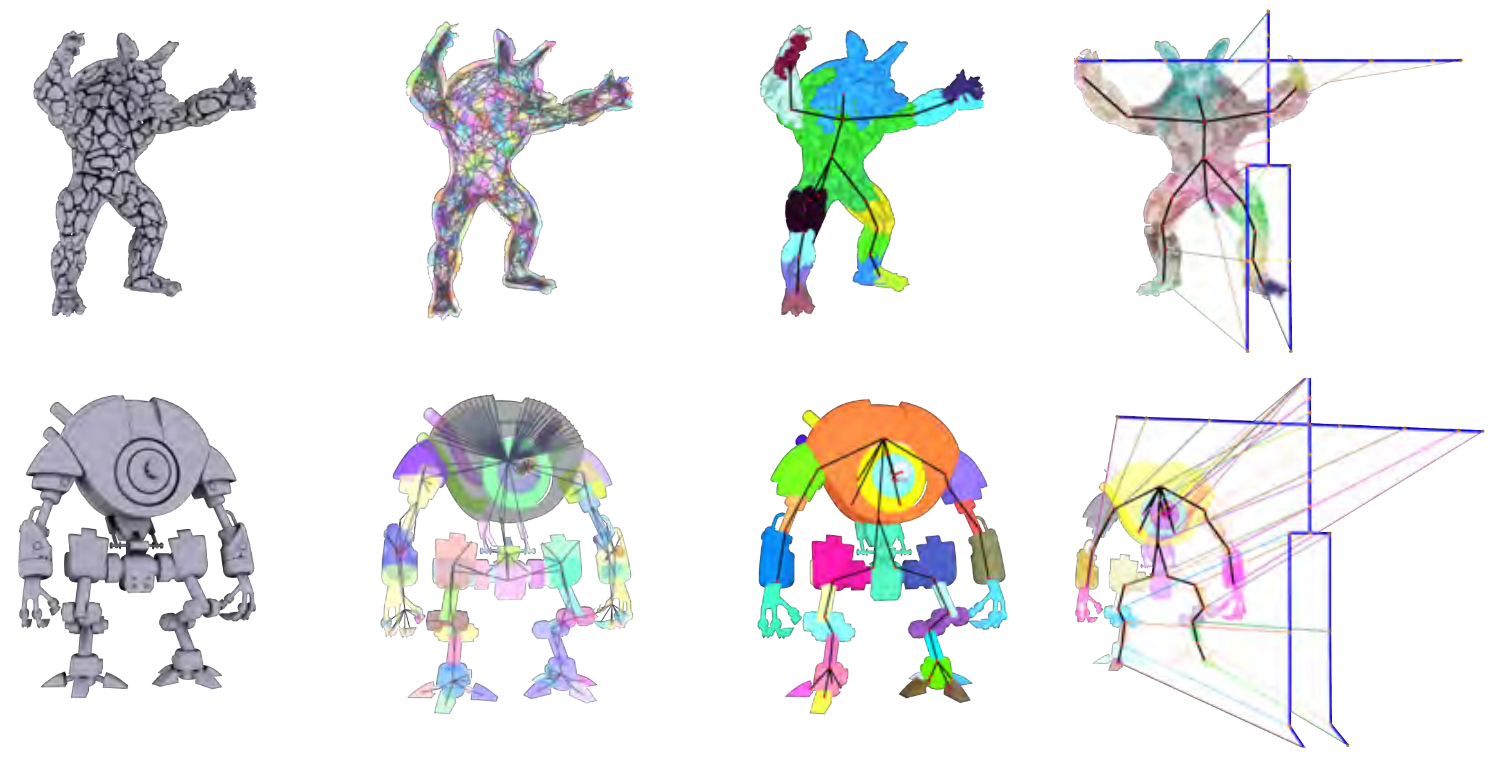
\includegraphics[width=15cm]{content/images/baharaj}
	\caption{Two multi component models rigged by the approach of Bharaj et.al.  \cite{Bharaj2012}.} 
	\label{fig:bharaj}
\end{figure}

\subsubsection{Manual rigging}

Manual rigging is the process to define the position of a predefined skeleton or armature in a mesh or volume. The user has to first define the skeleton and than to drag the joints and the bones into the model in order to define the rigging of it. Finet et.al. introduced a software called Bender which is open source software used for efficient model posing and morphing \cite{Finet2014Bender:Morphing}. One of their modules is called Armatures and enables the user to rig a model by defining or loading an armature in the *.vtk format and afterwards also saving the result. The armature can be represented in different ways using lines, cylinders or octohedrons. The armature parts are defined from a head to a tail. The head is normally connected to another armature part unless it is the first one. The tail may not be connected e.g. in case of the feet or the hands. The armature created has a hierarchy which can be defined individually. Each part of the armature can have a name. An example armature and the software are shown in Figure \ref{fig:Armatures}.

\begin{figure} [htb!]
    \centering
	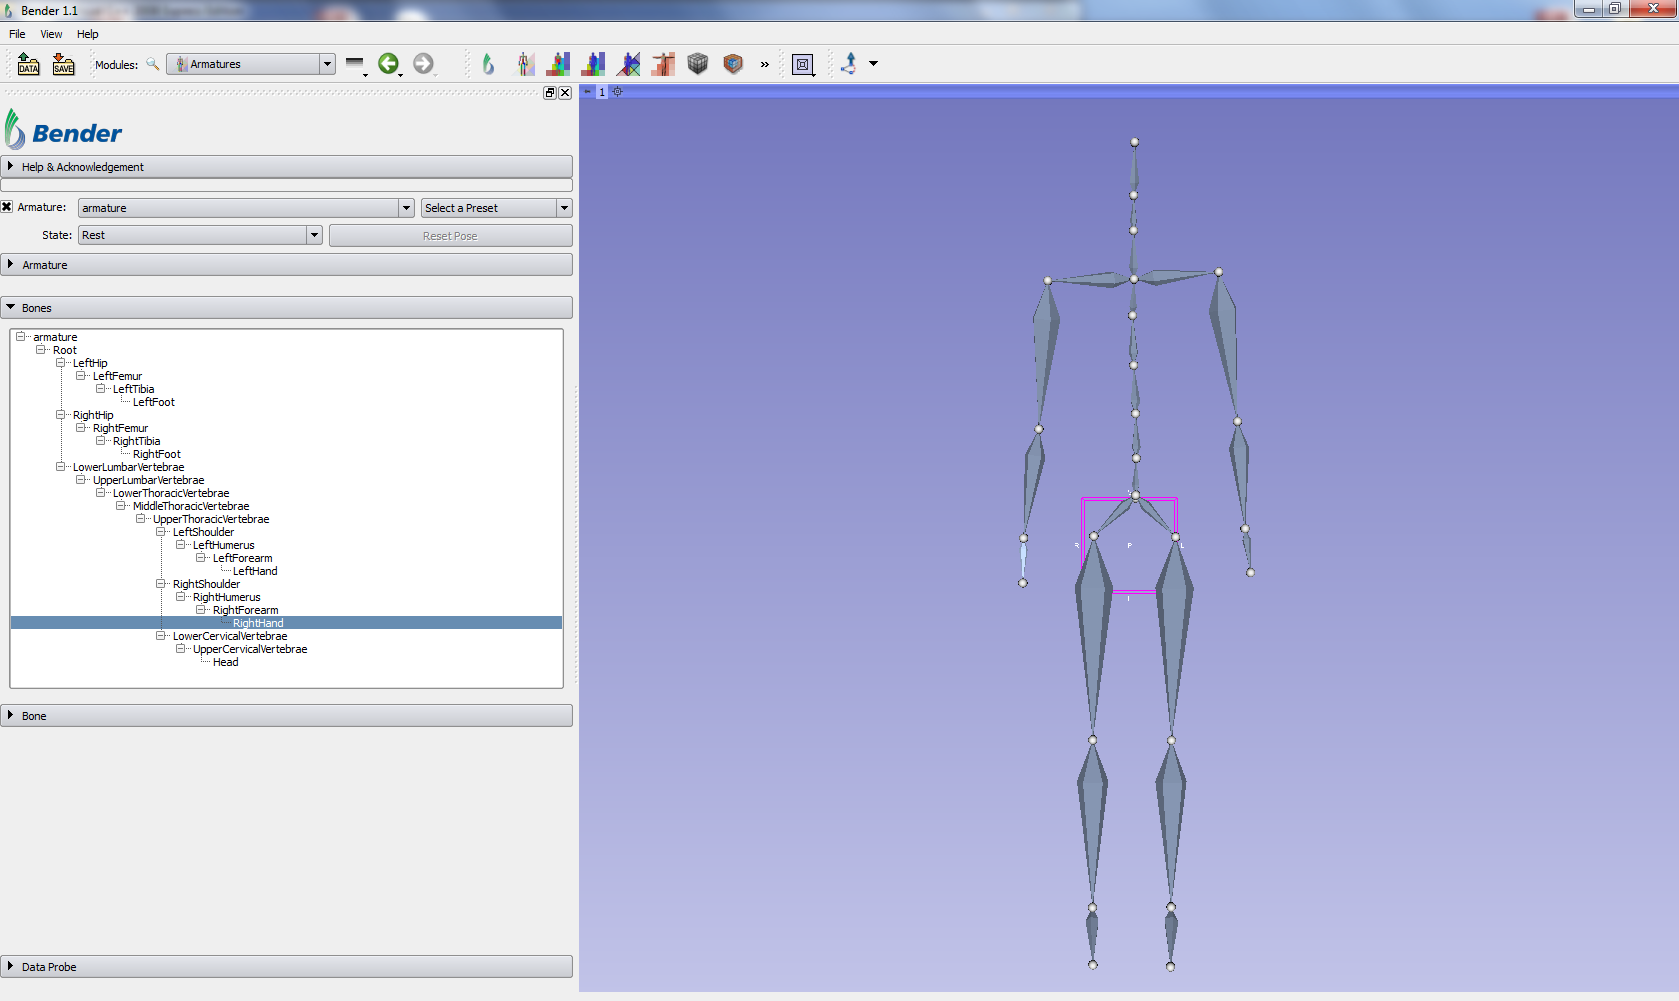
\includegraphics[width=14cm]{content/images/Armatures}
	\caption{Screenshot of the armature module of Bender. The shown armature is only en example and can be individually customized and generated. The screen is also used to drag the armature into the model if a model is loaded \cite{Andruejol2014BenderModules}.} 
	\label{fig:Armatures}
\end{figure}

\newpage
\section{Skinning or weighting of the armature}

After the armature or the skeleton is defined and the position inside of the mesh or volume has been found the data has to be weighted. That means that either the mesh or the voxels have to be linked to parts of the armature in order to know which parts have to be moved or transformed to create an animation or simply a movement. Some rigging approaches which originate from skinning the data already have this information available because during the skinning process the program simply has to save which voxels have to be removed in order to create parts of the skeleton. Afterwards these voxels are those who belong to the specific parts of the armature. One approach that is well known and has been introduced by Magnenat-Thalmann et.al. is called \gls{lbs}. The principal behind the algorithm is that between two adjacent points of the armature there can be a so called heat distributed plotted. This distribution can be used in order to define which mesh or voxel parts are deformed or affected by a movement of the given segment. Figure \ref{fig:lbs} visualizes how the \gls{lbs} works.

\begin{figure} [htb!]
    \centering
	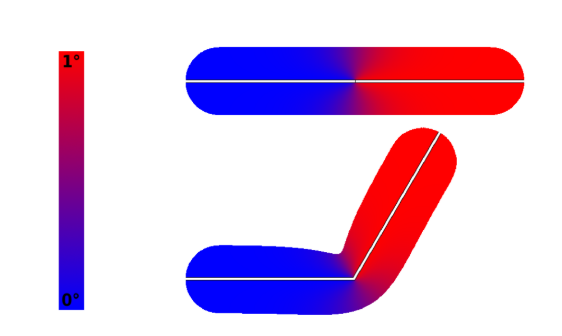
\includegraphics[width=10cm]{content/images/lbs}
	\caption{The left side of the image represents the heat distribution between two points which can also be seen at the top. The lower parts shows how the e.g. voxels will be affected if the right part of the joint moves about 45 degrees \cite{Baran2007}.} 
	\label{fig:lbs}
\end{figure}

\newpage

In case of the topological approach introduced by \cite{Bharaj2012} the skinning is already available because it is well known how the data have been abstracted in order to generate the point cloud, the graph and at the end the tree. The skinning of their approach also conforms the \gls{lbs} approach. The Pinocchio prototype uses the \gls{lbs} method to calculate for each vertex of the mesh the weight how it is affected by a bone transform. It is stated that it is highly affected by the distance to the bone and the interaction between two bones is calculated by using the \gls{lbs} method \cite{Baran2007}.

\subsection{Geodesic voxel binding}

Dionne and Lasa introduced the geodesic voxel binding as a voxel weighting approach in order to be able to transform voxel based characters using an armature \cite{Dionne2013GeodesicMeshes}. The authors state that their approach is particularly useful when having data that is not represented by a watertight mesh. They use the geodesic distance between each voxel and the nearest bone from the skeleton in order to determine which voxel is affected by which bone. The benefit is that the mash does not have to perfect and the complexity of the calculation is low and therefore fast \cite{Dionne2013GeodesicMeshes}. The process described by the authors is shown in Figure \ref{fig:geodesic}.

\begin{figure} [htb!]
    \centering
	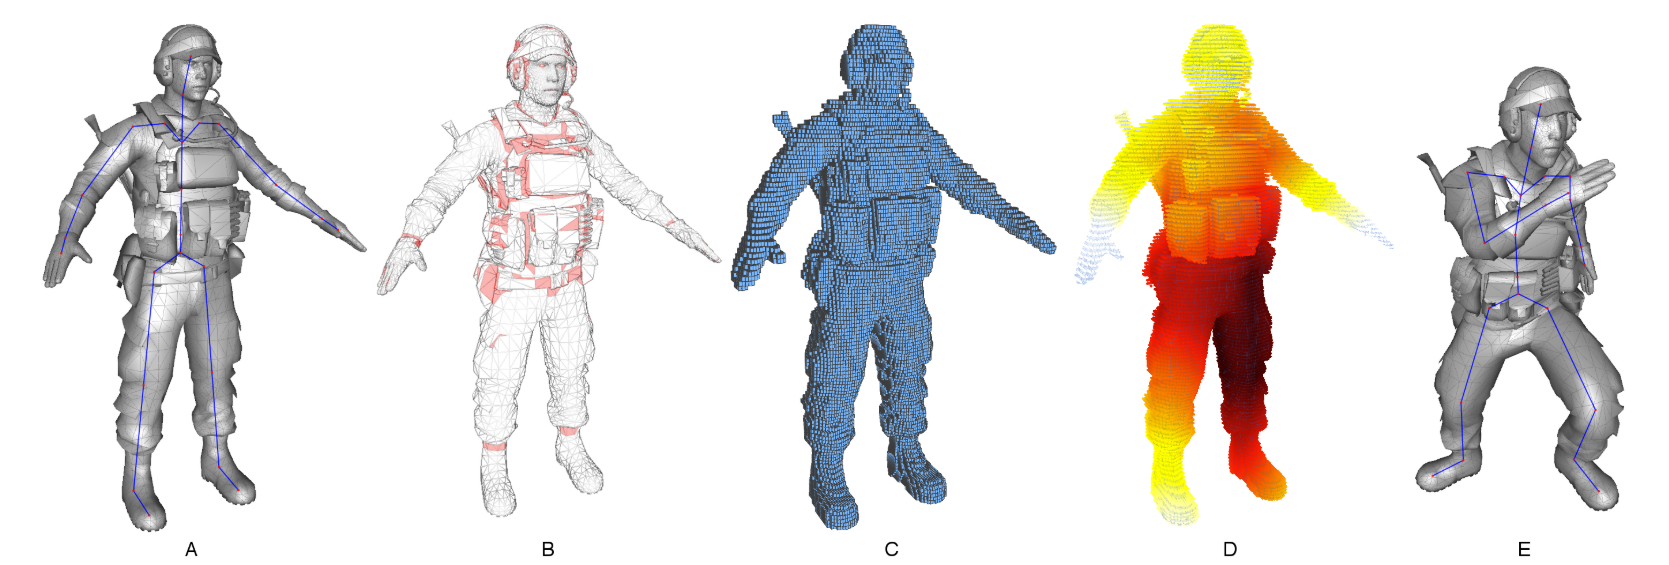
\includegraphics[width=13cm]{content/images/geodesic}
	\caption{This image represents the whole processing pipeline from the mesh at the beginning over the voxelized model in the middle, the geodesic representation at position D and the transformed mesh at the right hand side. Position B represents that there are some imperfections in the mesh which make it not watertight and therefore unsuitable for different skinning approaches \cite{Dionne2013GeodesicMeshes}.} 
	\label{fig:geodesic}
\end{figure}

\newpage

\subsubsection{Bender VolumeSkinning}

Bender has a volume skinning module which takes the volume as an input and an predefined armature \cite{Finet2014Bender:Morphing}. It then calculates the weights an delivers as output a new volume where the voxels are identified by the IDs of the armature parts they belong to. The mapping between armature parts and the voxels belonging to it are represented using different colors. One example output of the bender software is shown in Figure \ref{fig:BenderVolumeSkinning}.

\begin{figure} [htb!]
    \centering
	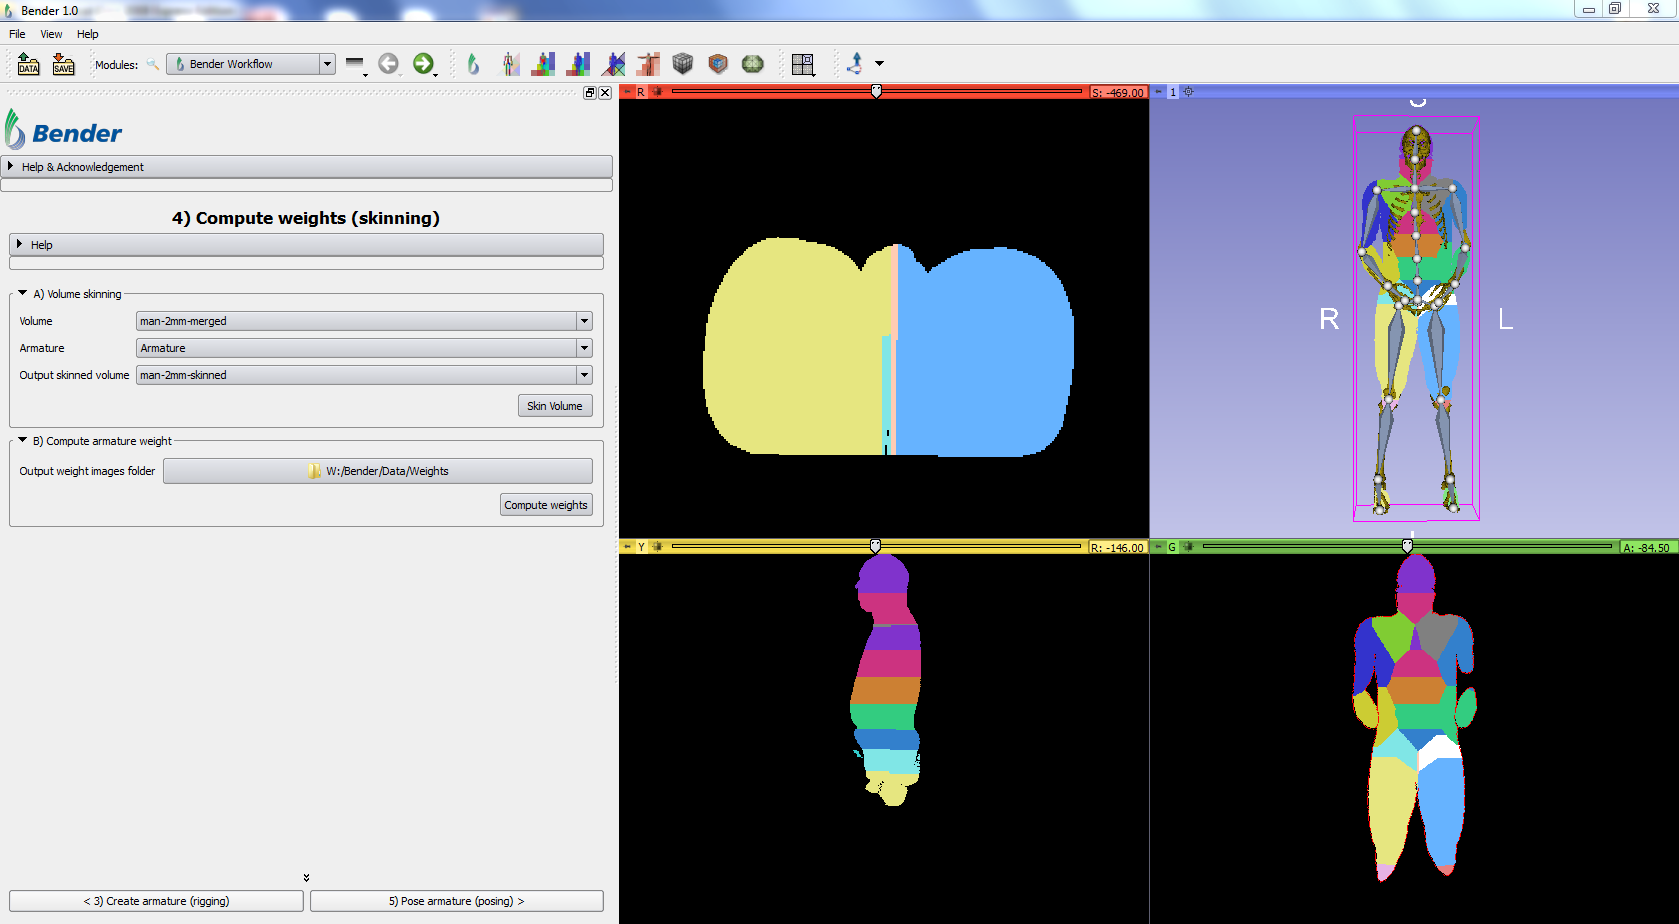
\includegraphics[width=13cm]{content/images/BenderVolumeSkinning}
	\caption{The Bender VolumeSkinning module with an example output of the armature and the skinned volume depicted in different colors representing which parts of the model belong to which armature part \cite{Andruejol2014BenderModules}.} 
	\label{fig:BenderVolumeSkinning}
\end{figure}

\section{Reformation of volumetric data}

The reformation of volumetric data can be performed in different ways. Some possibilities are shown in this sections.

\subsection{VolEdit}

Singh and Silver have introduced a method to manipulate volumetric data by using the \gls{ik} skeleton \cite{Singh2004}. After having identified the skeleton in the data and the joints of the skeleton they can use their software to manipulate the volume. One approach is to transform the skeleton using rotations around a joint. They are able to move each segment of the skeleton individually in respect to the according joint. In their approach the authors are using a program called VolEdit to modify the volumetric data \cite{Singh2004}. A simple interaction can be to apply a  transfer function to different parts of a model and to combine them. Figure \ref{fig:lobster} represents a lobster model which has been transformed using two different transfer functions in order to move the arms of the animal away from the body.

\begin{figure} [htb!]
    \centering
	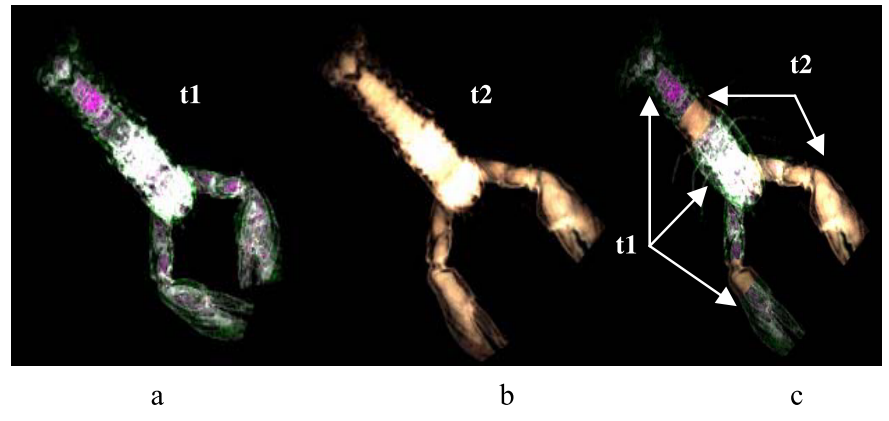
\includegraphics[width=13cm]{content/images/lobster}
	\caption{The lobster model transformed with two different transfer function which are applied to different regions of the model in order to move the arms away from the body \cite{Singh2004}.} 
	\label{fig:lobster}
\end{figure}

Using the same software VolEdit the authors also showed another example where they tried to unbend a rat which has been pictured in a small housing. This technique can be used to bring pictures into a standardized form like used in this thesis \cite{D.SilverK.yawsC.CorreaW.HurtP.Mason2005VolumetricSimulations}. Figure \ref{fig:mouse} shows the rat example before and after the unbending. Another interesting approach of Singh and Silver is to do a so called juxtaposition of different data sets. Using their program they are able to exchange the arm of a man by the arm of a lobster and the result looks quite promising. The application of the juxtaposition is depicted in Figure \ref{fig:juxtaposition}.

\begin{figure}
    \centering
	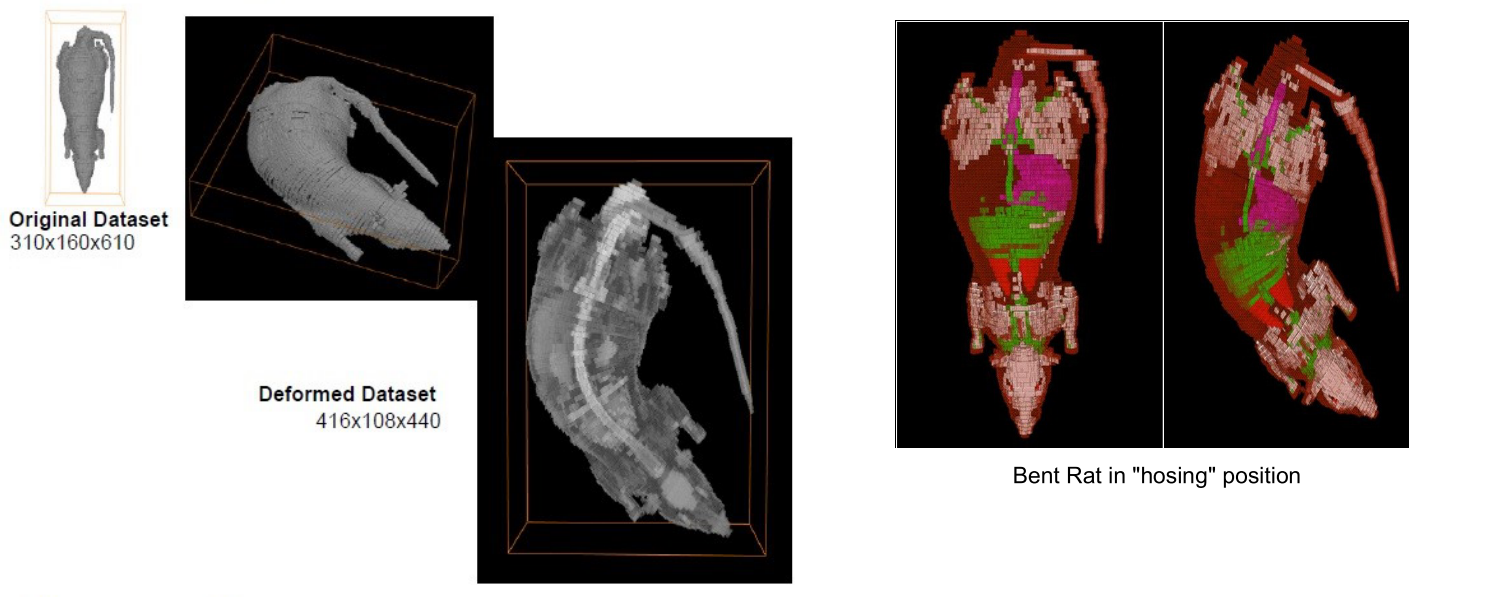
\includegraphics[width=13cm]{content/images/mouse}
	\caption{Unbending of a rat which is capt in a small housing \cite{D.SilverK.yawsC.CorreaW.HurtP.Mason2005VolumetricSimulations}.} 
	\label{fig:mouse}
\end{figure}

\begin{figure}
    \centering
	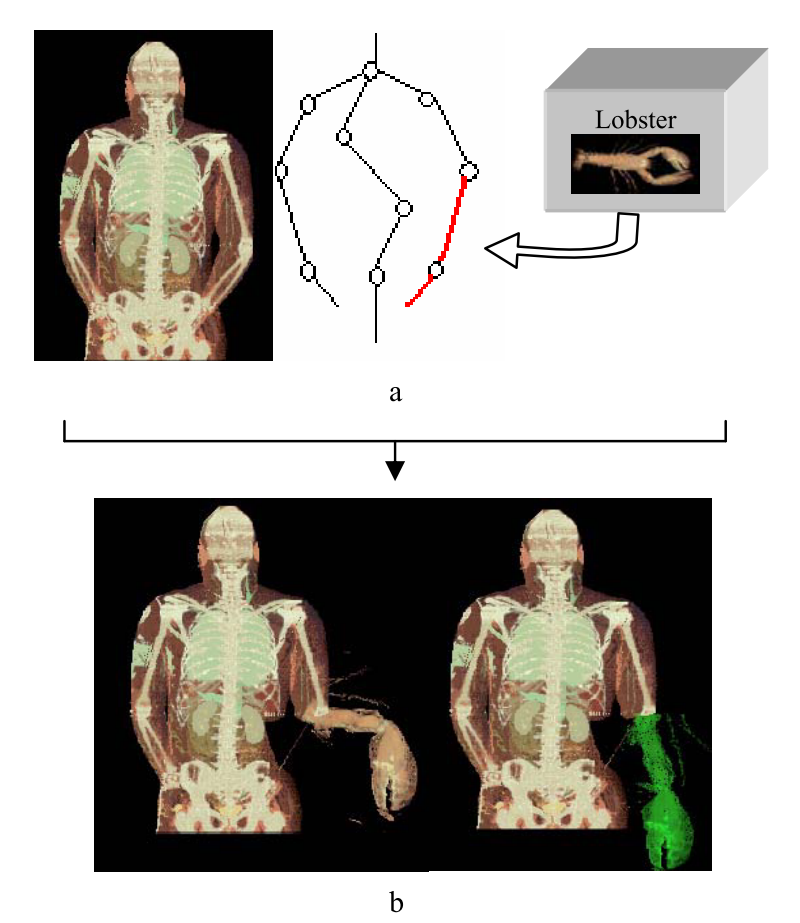
\includegraphics[width=10cm]{content/images/juxtaposition}
	\caption{Juxtaposition of the arm of a man and the arm of a lobster \cite{Singh2004}.} 
	\label{fig:juxtaposition}
\end{figure}

\subsection{Volume manipulation for surgical processes}

Nakao and Minato represent in their paper a novel techniques which can be used by surgeons to prepare for their surgical process or to share their knowledge in an interactive and visual appealing way \cite{Nakao2010}. In their application the user is able to manipulate patient specific volumetric data according to a real surgical intervention. The authors used \gls{ct} and \gls{mri} images as a source for their method and enable the user to perform physically correct modelled surgical procedures. The used a vertices based grid and finite element analysis in order to create a visualization that behaves physical correctly \cite{Nakao2010}.  An example for such a surgical intervention and the volumetric rendering can be seen in Figure \ref{fig:physical}.

\begin{figure} [htb!]
    \centering
	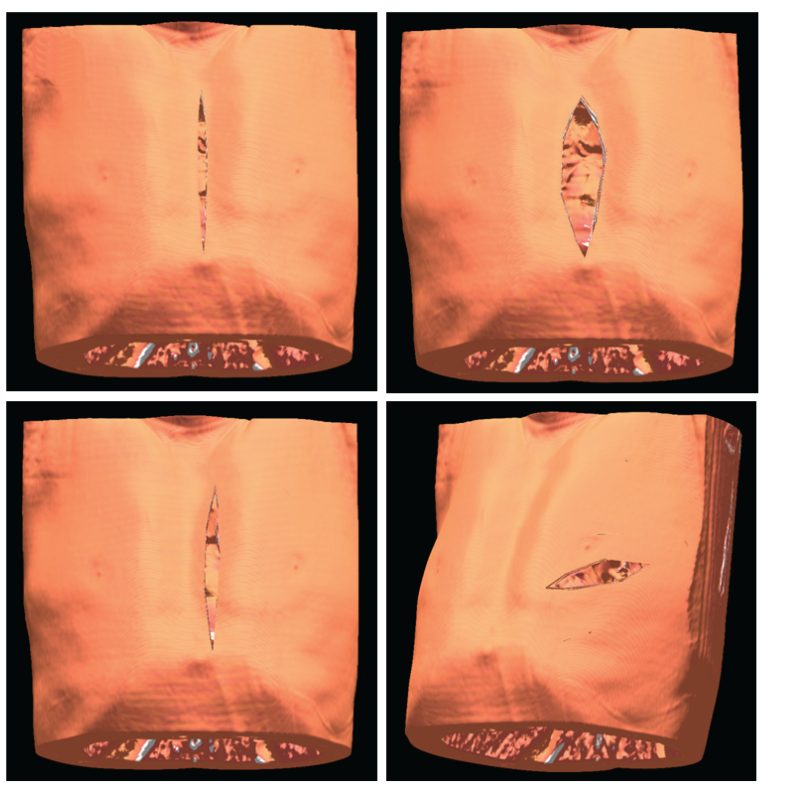
\includegraphics[width=11cm]{content/images/physical}
	\caption{Visualization of a volume cutting considering the tension that arises from the surrounding tissue resulting in a cleft with a differing size \cite{Nakao2010}.} 
	\label{fig:physical}
\end{figure}
\newpage

\chapter{Fetalformation (title in progress)}\label{ch:methods}
\newacronym{vtk}{VTK}{visualization toolkit}

In this section the methods used to accomplish the aims of the application are presented. The sections are ordered after the workflow the user has to perform. Not only the methods which are really used in the resulting application will be described also alternative approaches which may have not found their way into the final solution will be presented. It will also be described why and how we have decided which approaches fit best for the solution.

\section{Application overview}

In the first section the aim is to give the reader an overview of the presented methods. Figure \ref{fig:methodsOverview} shows the workflow of the application. The first step is loading of the data. This step can be very complex because it highly depends on the format the data are provided. In case of ultrasound data originating from an clinical investigation or already registered data representing the whole fetus, the data format might be \gls{dicom}. Another possibility would be to provide the data using a *.raw format which only include the data itself and no surrounding information which e.g. \gls{dicom} includes. The *.raw format might come along with a *.mhd file which is also called the MetaHeader and represents meta information about the data included in the *.raw file. The data might also come in various other formats and therefore there might be some restrictions. Thinking about loading data the usage of the tools MeVisLab \cite{AGMeVisLab} or 3D Slicer \cite{Slicer3DSlicer, Fedorov20123DNetwork} is endorsed. Both software solutions are publicly available, open source and for free.\newline

\begin{figure}
    \centering
	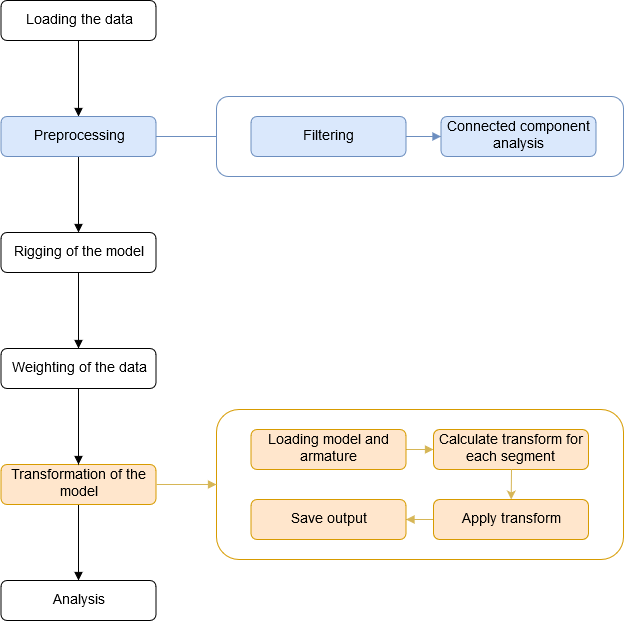
\includegraphics[width=15cm]{content/images/MethodsOverview}
	\caption{The application overview represents the pipeline that has to be performed in order to result in a T-pose fetal representation.} 
	\label{fig:methodsOverview}
\end{figure}

The next step is called preprocessing and depends highly on the input data. The data can be visualized in different applications like MeVisLab or 3D Slicer. The preprocessing pipeline used in this thesis includes a threshold processing be able to distinguish between background data and the data belonging to the fetus. The next step is to calculate the larges connected component in the data and get rid of all other information in the dataset. The output of this step is a volume only holding information about the fetus.\newline

One of the larger and also very important steps is to rig the data. This step can be performed in lots of different ways. One solution might be to use the Bender software which is based on 3D Slicer and the paper about it has been written by Finet et.al. \cite{Finet2014Bender:Morphing}. Bender is also an open source program which includes various modules for model posing and morphing. One model is called armature and can be used to create and place an armature in a model.\newline

The next step in the pipeline describes the weighting or skinning of the data. This processing step is used to calculate the contribution of different segments of the armature to the input data namely the volumetric data of the fetus. The output of this processing step is a volume which includes the mapping for each voxel to one of the armature segments. This step might also be performed using Bender \cite{Finet2014Bender:Morphing}. In Bender the module VolumeSkinning shall be used which needs as input the armature and the volume. The result will be just the described one.\newline

The most unique and novel part of the pipeline is the transformation of the model. This processing step is used to actually transform the data. The transformation is performed automatically. As an import the armature and the volumetric data is required. The volume has to be weighted and each segment of the armature has to be mapped to some voxels. The transformation calculates the needed transformations of each segment in respect to the adjacent ones, resulting in a fetus model at a T-position. As represented in the overview Figure \ref{fig:methodsOverview} with a dashed line the transformation of the model might result in a feedback loop back to the rigging. The user might want to reset some joint positions in order to get a more realistic and representative result in the end. The transformation will be described in greater detail in the section \ref{sec:transformation}. The output of the transformation can be in different file formats but it is recommended to choose a well known form in order enable the analysis to be performed in different consumer products.\newline

The last step of the pipeline is named analysis and has the aim to gather insight in the now transformed data. A part of the analysis step could be automatically done e.g. some measurements like the finger to finger span or the head to toe length. The user gets new insights in this module and is be able to interactively view the now unfolded data. Taking measurements like specific circumferences or lengths like the femur length for example should be possible. This module can be very user specific because it depends on the preferences of the user and which modules they would like to use. Having a nice rendering of the volumetric data might also be interesting where approaches using the \gls{gpu} might be interesting. One example is the GVDB library by NVIDIA which is particularly written for voxel visualization \cite{Hoetzlein2016}.

\section{Loading the data}

Loading the medical or phantom data is a step which occurs not only once during the processing of the data. Some processing steps of the pipeline may not be implemented using the same system and therefore data exchange namely loading and generating output is essential. Loading of the data somehow differs between the modalities used. In this section the loading steps which are used in this thesis are described.\newline

\subsection{MeVisLab}

The first loading step is performed in MeVisLab \cite{AGMeVisLab}. MeVisLab is a tool which consists of a large amount of modules which the user can choose. Certainly there are many different modules to load data. In this thesis two can be used namely the $ImageLoad$ or the $LoadAny$ module. The $ImageLoad$ module and the corresponding properties can be seen in Figure \ref{fig:meImageLoad}. The $ImageLoad$ module is used to examine *.raw data but the user has to define the spatial resolution and the data type which is included in the *.raw file.

\begin{figure} [!htb]
    \centering
	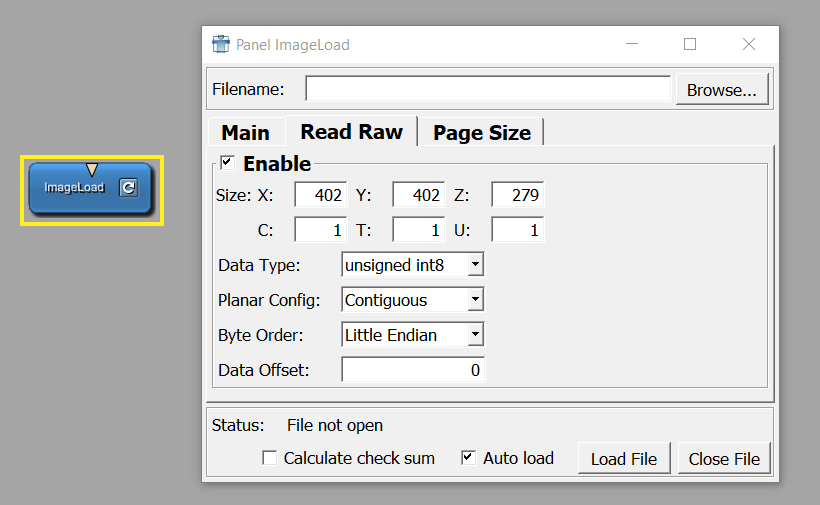
\includegraphics[width=10cm]{content/images/meImageLoad}
	\caption{The screenshot shows the $ImageLoad$ module and the corresponding settings where the user has to define the resolution of the *.raw file and the data type.} 
	\label{fig:meImageLoad}
\end{figure}

If the data is present in a *.mhd file format one might just use the $LoadAny$ module. This module has the benefit that the user does not have to apply any settings but the file has to support being loaded. A *.raw file might not be loadable because the module does not have any contextual information included.

\begin{figure} [!htb]
    \centering
	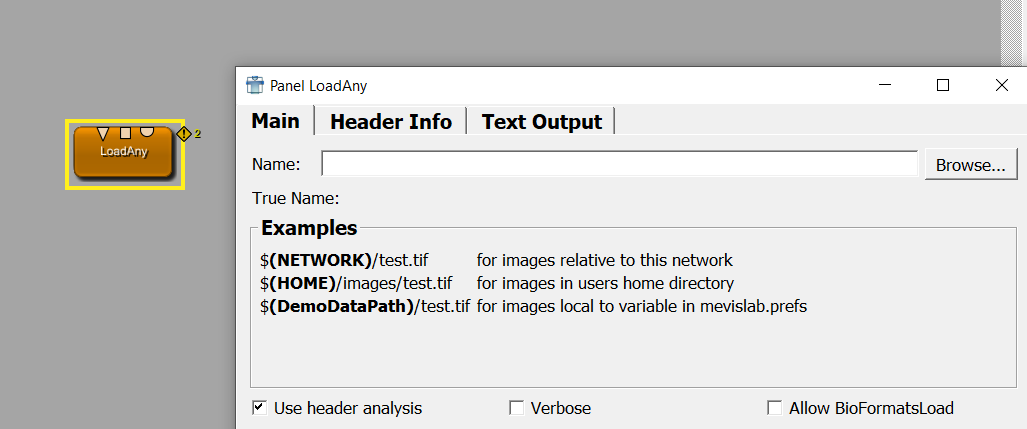
\includegraphics[width=12cm]{content/images/meLoadAny}
	\caption{The $LoadAny$ module of MeVisLab which can be used to load e.g. *.mhd files along with the corresponding *.raw file without having to set any properties.} 
	\label{fig:meLoadAny}
\end{figure}

\newpage
\subsection{3D Slicer and Bender}

3D Slicer \cite{Slicer3DSlicer,Fedorov20123DNetwork} as well as Bender \cite{Finet2014Bender:Morphing} which is a 3D Slicer based application do also provide to load the medical data and this option is used during this processing steps. Loading data is quite simple using those programs. Loading data in 3D Slicer is performed by clicking on the button highlighted in the Figure \ref{fig:slcLoad} and in Bender by clicking the button in Figure \ref{fig:bendLoad}. Both loading steps are simply performed by selecting the file to load, unfortunately both applicaions do not support loading files in *.raw format. The data is automatically available for visualization and further processing in the software.

\begin{figure} [!htb]
    \centering
	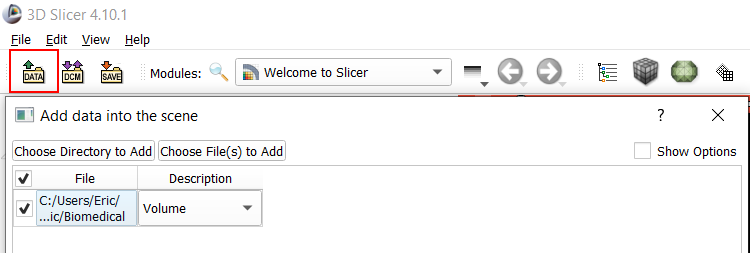
\includegraphics[width=12cm]{content/images/slcLoad}
	\caption{Loading of data in to the 3D Slicer program.} 
	\label{fig:slcLoad}
\end{figure}

\begin{figure} [!htb]
    \centering
	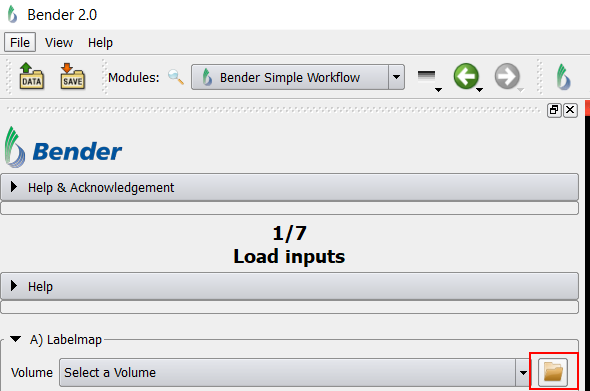
\includegraphics[width=8cm]{content/images/bendLoad}
	\caption{Loading data for being processed in Bender.} 
	\label{fig:bendLoad}
\end{figure}

\subsection{Phantom data generation}

When thinking about a transformation of ultrasound data to a specific position the question arises how the approach should be validated. There is no ground truth so to say if the found transformation is good or bad. Therefore in this thesis a phantom approach has been used. The phantom data represents a human in a T-pose. The model can be transformed into different fetus like poses using Blender \cite{Foundation2019Blender}. Blender enables the user to perform the rigging process and afterwards use the Pose option in order to generate different poses to be tested with the introduced workflow. The model used in this thesis has been found in the internet and is licensed by the Royalty Free License with allows all extended usages and can be fond here \cite{Squidifier2010DetailedMan}. It has to be mentioned that Blender works with a mesh and therefore surface representation of the \gls{3d} models and this data would not be loadable. Therefore a processing step has to be performed to generate a voxelized model out of the mesh.

\subsubsection{STL generation}

The first step towards a voxelized model representation of a mesh is to export the mesh in the *.stl format which is supported by Blender off the shelf. One only has to select the option export as stl and this step is already done.

\subsubsection{STL to image stack}

After having generated the *.stl file of the mesh model the next step is to convert it into an image stack. During the work on this thesis a public available python script has been used namely $stl-to-voxel$ \cite{Pederkoff2015Stl-to-voxel}. This pyhton script transforms the *.stl mash format in a stack of images which can be interpreted as voxel values. The transformation into an actual \gls{3d} volume file is done in the next step using another tool. The python scrip has to be run with the *.stl file and a folder as input. In then generates the images. It might be useful if the resolution is increased by altering one line of code in the file $stltovoxel.py$. The list line number 99 defines the resolution of the image in x and y axis. The default value is 100 and for the data used during this thesis 400 seemed to be an appropriate value. An example input and output situation of the script is shown in Figure \ref{fig:stlToVoxel}.

\begin{figure} [!htb]
    \centering
	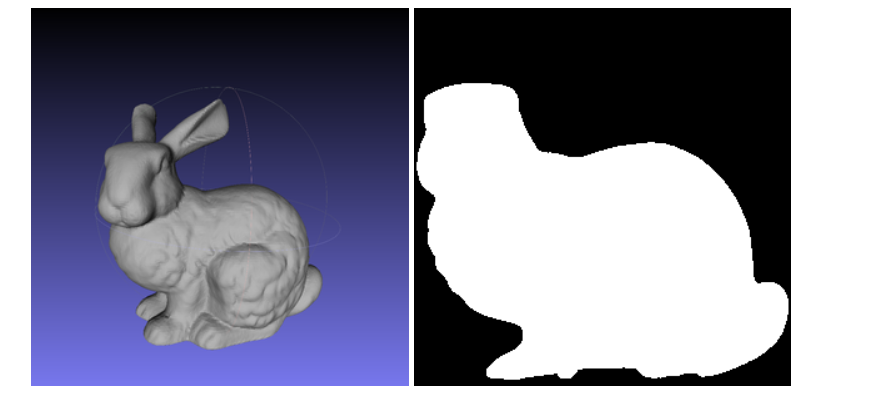
\includegraphics[width=14cm]{content/images/stlToVoxel}
	\caption{Example of the $stl-to-voxel$ python script showing the mesh representation on the left and one image of the image stack on the right.} 
	\label{fig:stlToVoxel}
\end{figure}

\newpage
\subsubsection{Convert image stack to *.raw file}

The last step in the phantom data generation is to convert the image stack given as an output form the $stl-to-voxel$ python script into an actual volumetric dataset. This step is performed using the tool ImageJ  \cite{Ecosystem2018ImageJ}. ImageJ is an open platform for scientific image analysis. The tool provides an import for the given image stack simply by selecting the option $File$ $Import$ and $Image Sequence$ and selecting the first image of the image stack. The *.raw file can be saved by selecting the option $Save As$ and $Raw Data$.

\newpage
\section{Preprocessing}

The preprocessing step depends as stated before highly on the data which has to be processed. In case of a fetal ultrasound investigation the data might be affected by artefacts and information which does not belong to the fetus. Cortes et.al. introduced in their paper a dataset of a phantom ultrasound investigation with artefacts included which may also arise in that way during a \gls{3d} fetal ultrasound investigation \cite{Cortes2016UltrasoundEvaluation}. In order to depict the preprocessing steps introduced in this section the publically available dataset of the authors will be used. The data example before the preprocessing can be seen in Figure \ref{fig:phantomFetusOr}.

\begin{figure} [!htb]
    \centering
	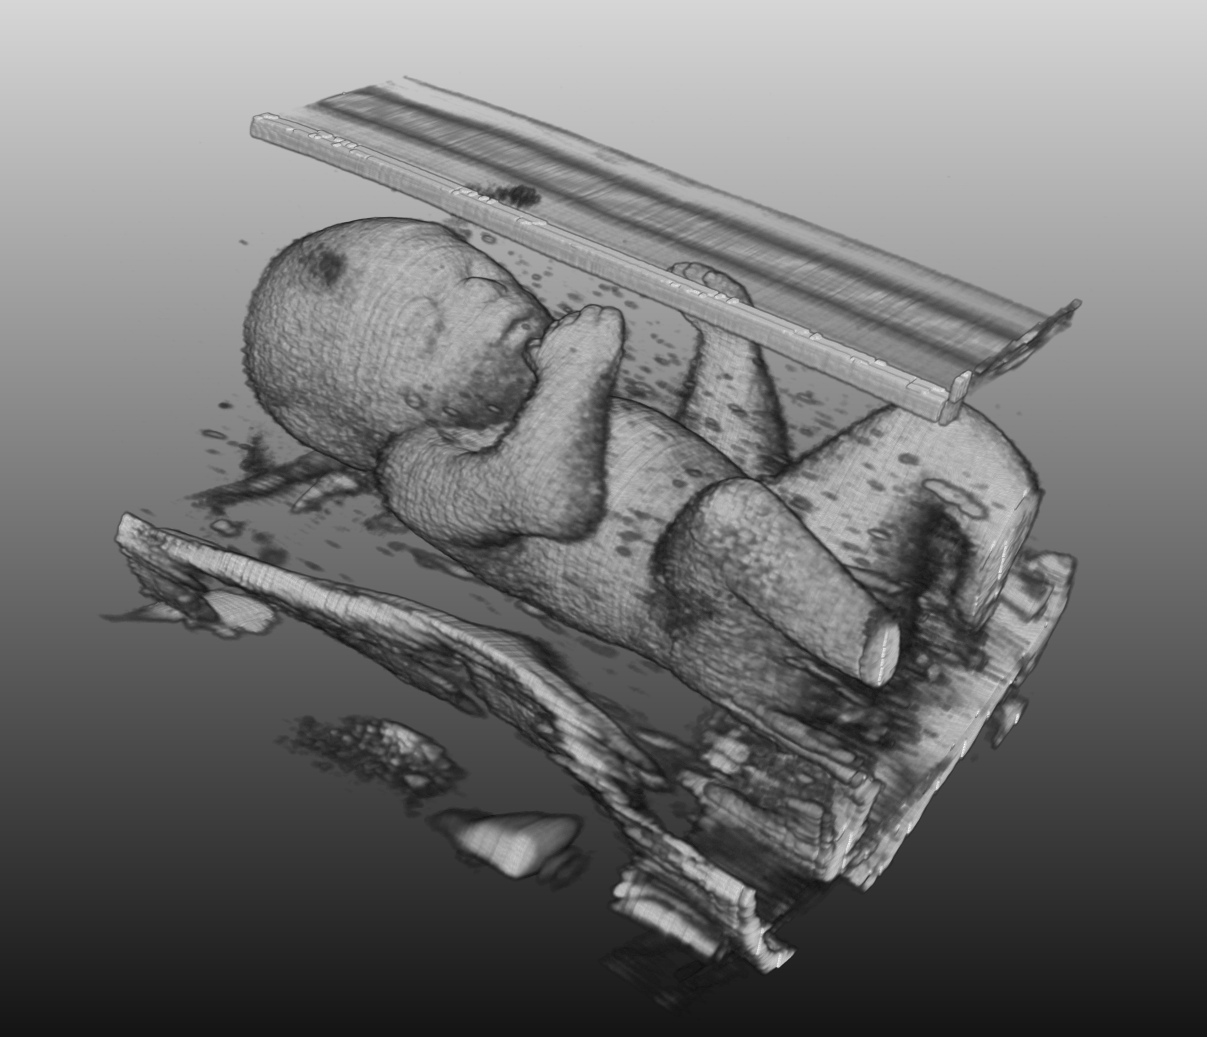
\includegraphics[width=8.5cm]{content/images/phantomFetusOr}
	\caption{The fetus phantom model data including arteficts which may also arise during a \gls{3d} fetal utlrasound investigation \cite{Cortes2016UltrasoundEvaluation}.} 
	\label{fig:phantomFetusOr}
\end{figure}

\newpage
\subsection{Filtering}

The first step is to apply a threshold. This operation is used to get rid of some of the artefacts in the data and to have a cleared view of the fetus. The module used in MeVisLab is called $Threshold$ and in the Figure \ref{fig:phantomFetusTh} a value of greater than 60 is used.

\begin{figure} [!htb]
    \centering
	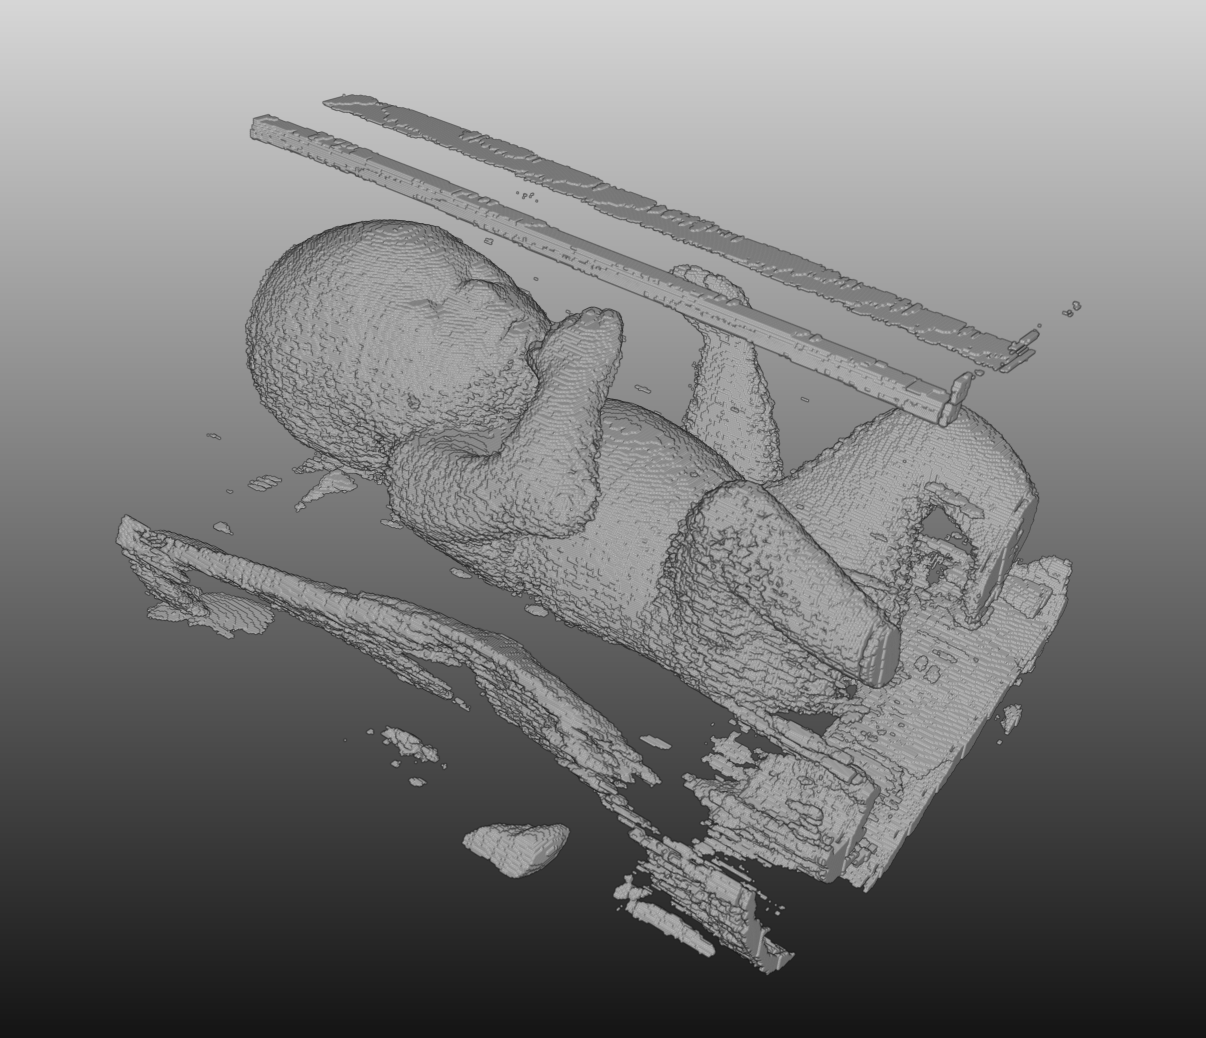
\includegraphics[width=8.5cm]{content/images/phantomFetusTh}
	\caption{The fetus phantom model after applying a threshold greater than 60.} 
	\label{fig:phantomFetusTh}
\end{figure}

\subsection{Connected component analysis}

The last step of the preprocessing pipeline is the so called largest connected component analysis. This step is used in order to get rid of all elements in the volumetric dataset, which are not connected to the fetus. It is defined that the fetus in the gathered ultrasound investigation data consists of one large component without any detached parts. The second thought is that in a fetus centered ultrasound investigation the fetus should of course be the largest component in the dataset. In order to calculate the largest connected component and filter the others three components are used namely $ComputeConnectedComponent$, $FilterConnectedComponents$ and $ConnectedComponentsToImage$. The first module takes the thresholded image data as an input and calculates the connected components. The second one is used to filter the components and search for the largest one by setting the $selectionMode$ to $Largest$. The last stated module finally converts the component back to image data which then can be visualized again. The result of this processing step can be seen in the following Figure \ref{fig:phantomFetusCCA}.

\begin{figure} [!htb]
    \centering
	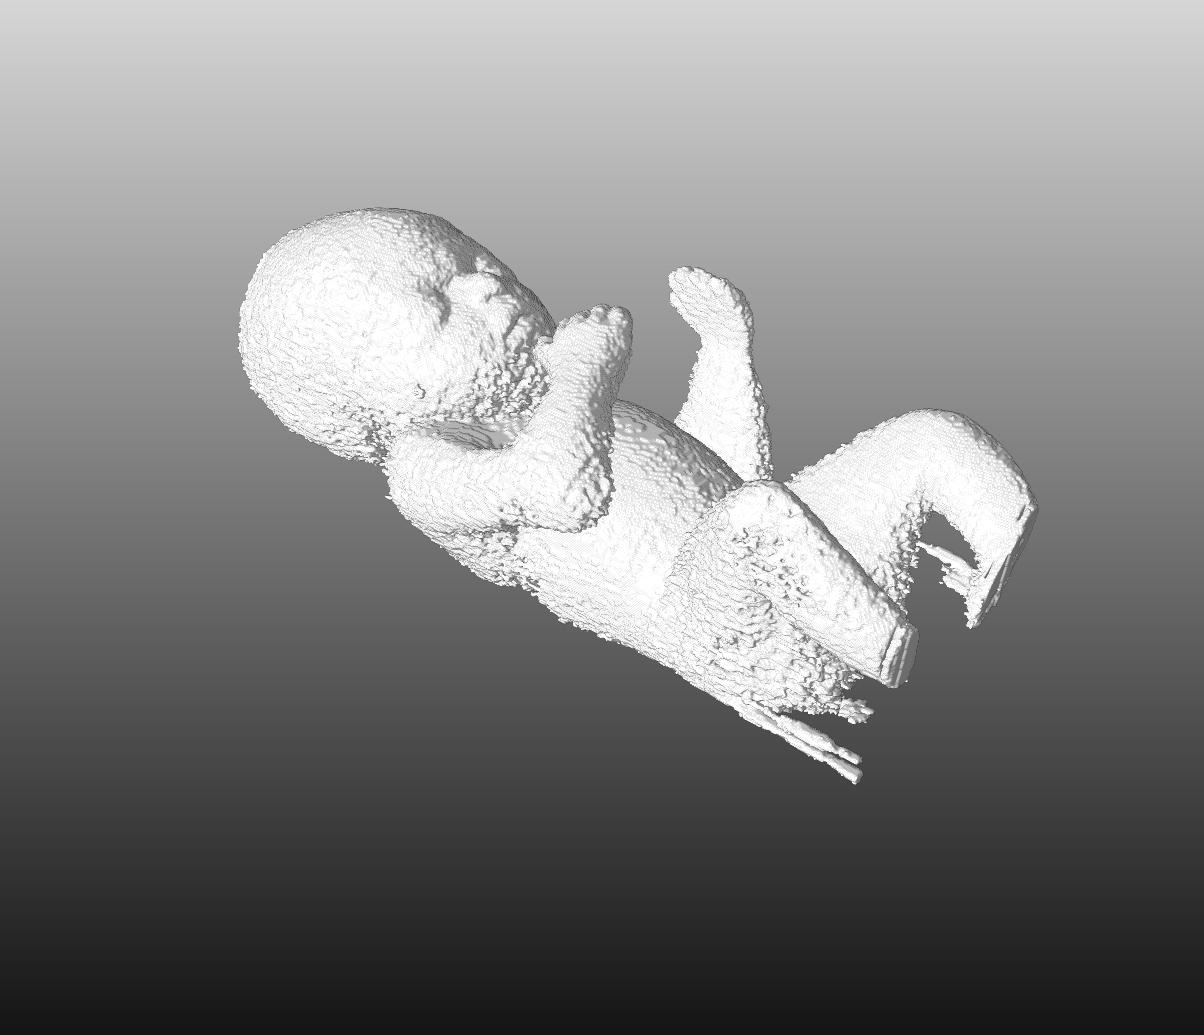
\includegraphics[width=8.5cm]{content/images/phantomFetusCCA}
	\caption{The fetus phantom model after applying a threshold greater than 60.} 
	\label{fig:phantomFetusCCA}
\end{figure}

\newpage
\section{Rigging of the model}\label{sct:rigging}

Rigging of \gls{3d} models can be done in many different ways, during this thesis the approach implemented by Bender \cite{Finet2014Bender:Morphing} has been used. The first step was to produce a template skeleton which is rather simple and does not provide too many segments that have to be included in the structure. When thinking of simplification a good tradeoff between losing details and having too less details has to be found. The Skeleton used in terms of this work is composed out of 20 segments and of 18 joints. Figure \ref{fig:Armature} shows a schematical representation of the produced armature. The representation of this armature in Bender can be seen in Figure \ref{fig:arm}.\newline

\subsection{Bender}
The rigging in Bender is done by simply dragging the skeleton piece by piece into the model. The \gls{3d} navigation has to be used in order to analyse if each part is correctly placed along each axis. The difficulty behind this approach is that in some cases the parts seem to be perfectly placed but when having a look in another representation the segments are not correct. The user has to check each segment along each axis and drag the segments until the place is correct along each axis. This procedure might seam tedeous and complex but unfortunately there have not been any known approaches to rig characters automatically that are already in a transformed position which differs completely from the known T-pose. Figure \ref{fig:rigging} represents the input of the rigging process and the result.

\begin{figure} [!htb]
    \centering
	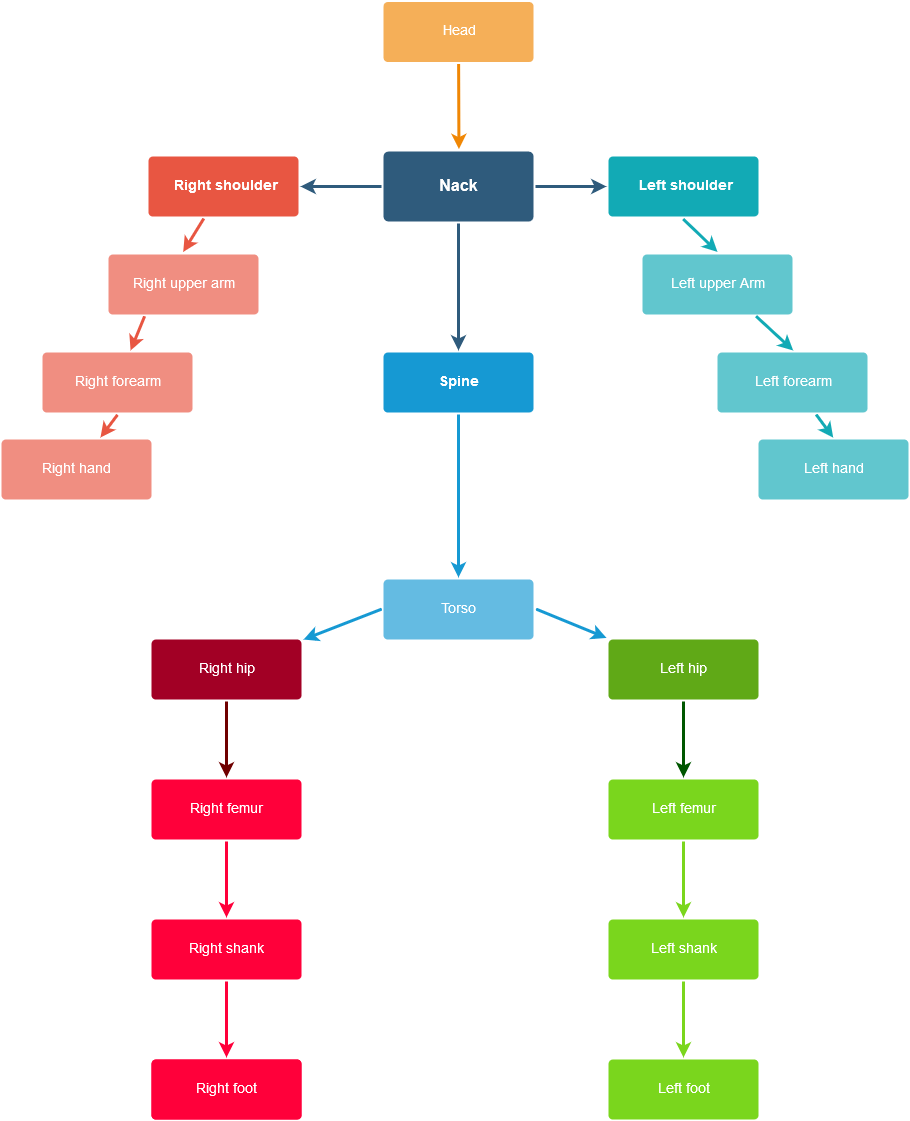
\includegraphics[width=14cm]{content/images/Armature}
	\caption{Schematical representation of the armature used in bender consisting of 20 segments and 18 joints.} 
	\label{fig:Armature}
\end{figure}

\begin{figure} [!htb]
    \centering
	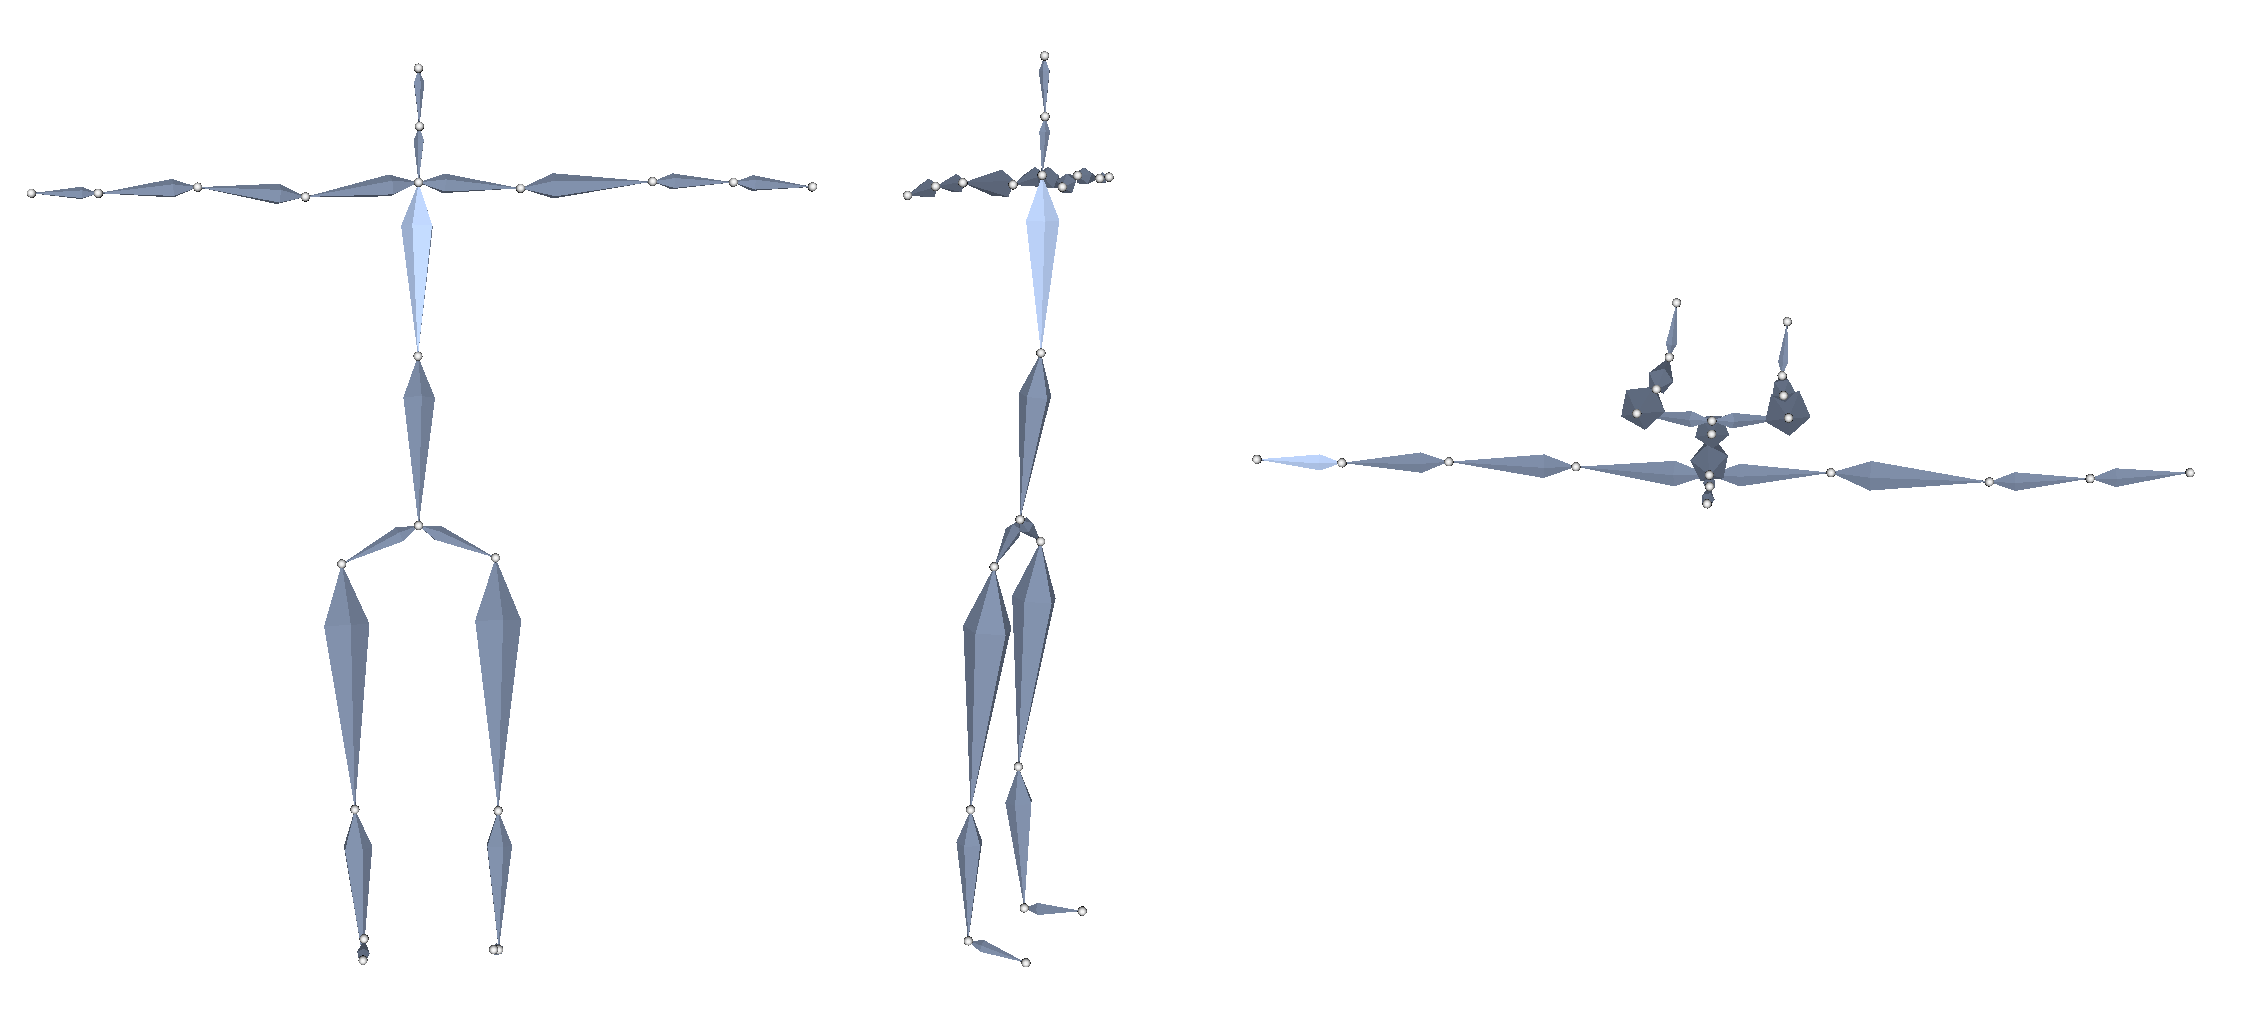
\includegraphics[width=15cm]{content/images/arm}
	\caption{Representation of the template armature in a T-position in Bender using a octohedronal representation} 
	\label{fig:arm}
\end{figure}

\begin{figure} [!htb]
    \centering
	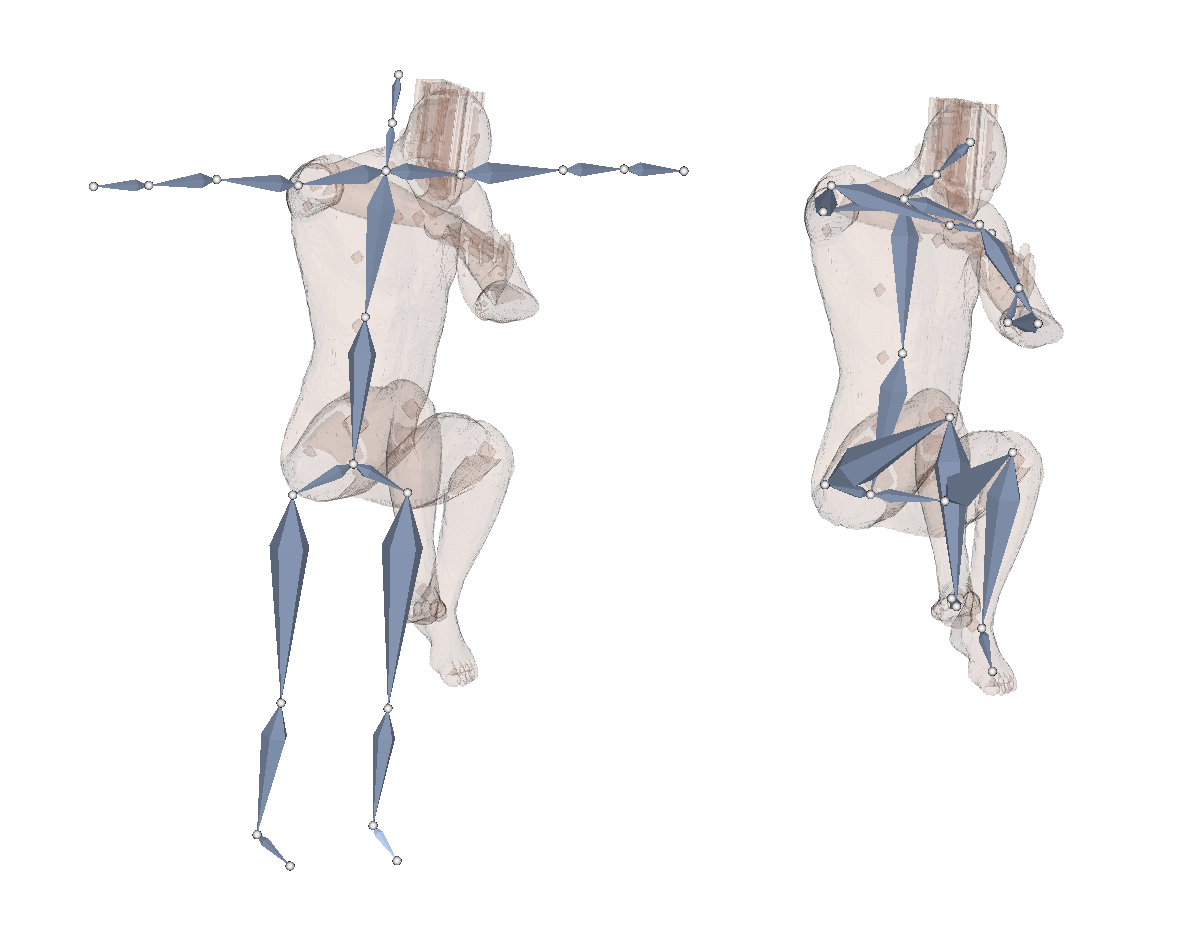
\includegraphics[width=12cm]{content/images/rigging}
	\caption{On the left side of the picture a phantom model of a man and the armature representation in Bender can be seen. The right image shows the result namely the armature perfectly in place.} 
	\label{fig:rigging}
\end{figure}

\newpage
\subsection{GPU based voxel visualization}

Another approach of rigging the data would be to implement a way to identify and work with keypoints of the model and automatically incorporate the armature. Therefore one approach might be to use a \gls{gpu} based approach to visualize and analyse the data. NVIDIA introduced in 2016 a \gls{gpu} based voxel database called GVDB which can be used as an efficient data structure for voxel visualization \cite{Hoetzlein2016}. Their approach is open source looked promising as a starting point for the tasks in this master thesis. First the visualization aspect has been analysed and worked out well. The example section of NVIDIA provided an out of the box loading algorithm which can be used in terms of *.raw data and the loading worked perfectly.\newline
In this work a simple and new approach has been introduced to select data based on a abstract representation of the voxel data. GVDB provides different abstraction levels which have been used in order to select parts of the voxelized model interactively using the three axis. The user had the option to move with the mouse and select a starting and an ending point along each axis to summarize six selections. The result would be a very simple selection process resulting in the selection of a specific part of the model which than would be highlighted. The selection process and the highlighted section of the data is depicted in Figure \ref{fig:gvdb}. The approach was unfortunately not used in the end because there was no option how to apply transformations to only parts of the model which would have been needed in order to transform the data to a T-pose.

\begin{figure} [!htb]
    \centering
	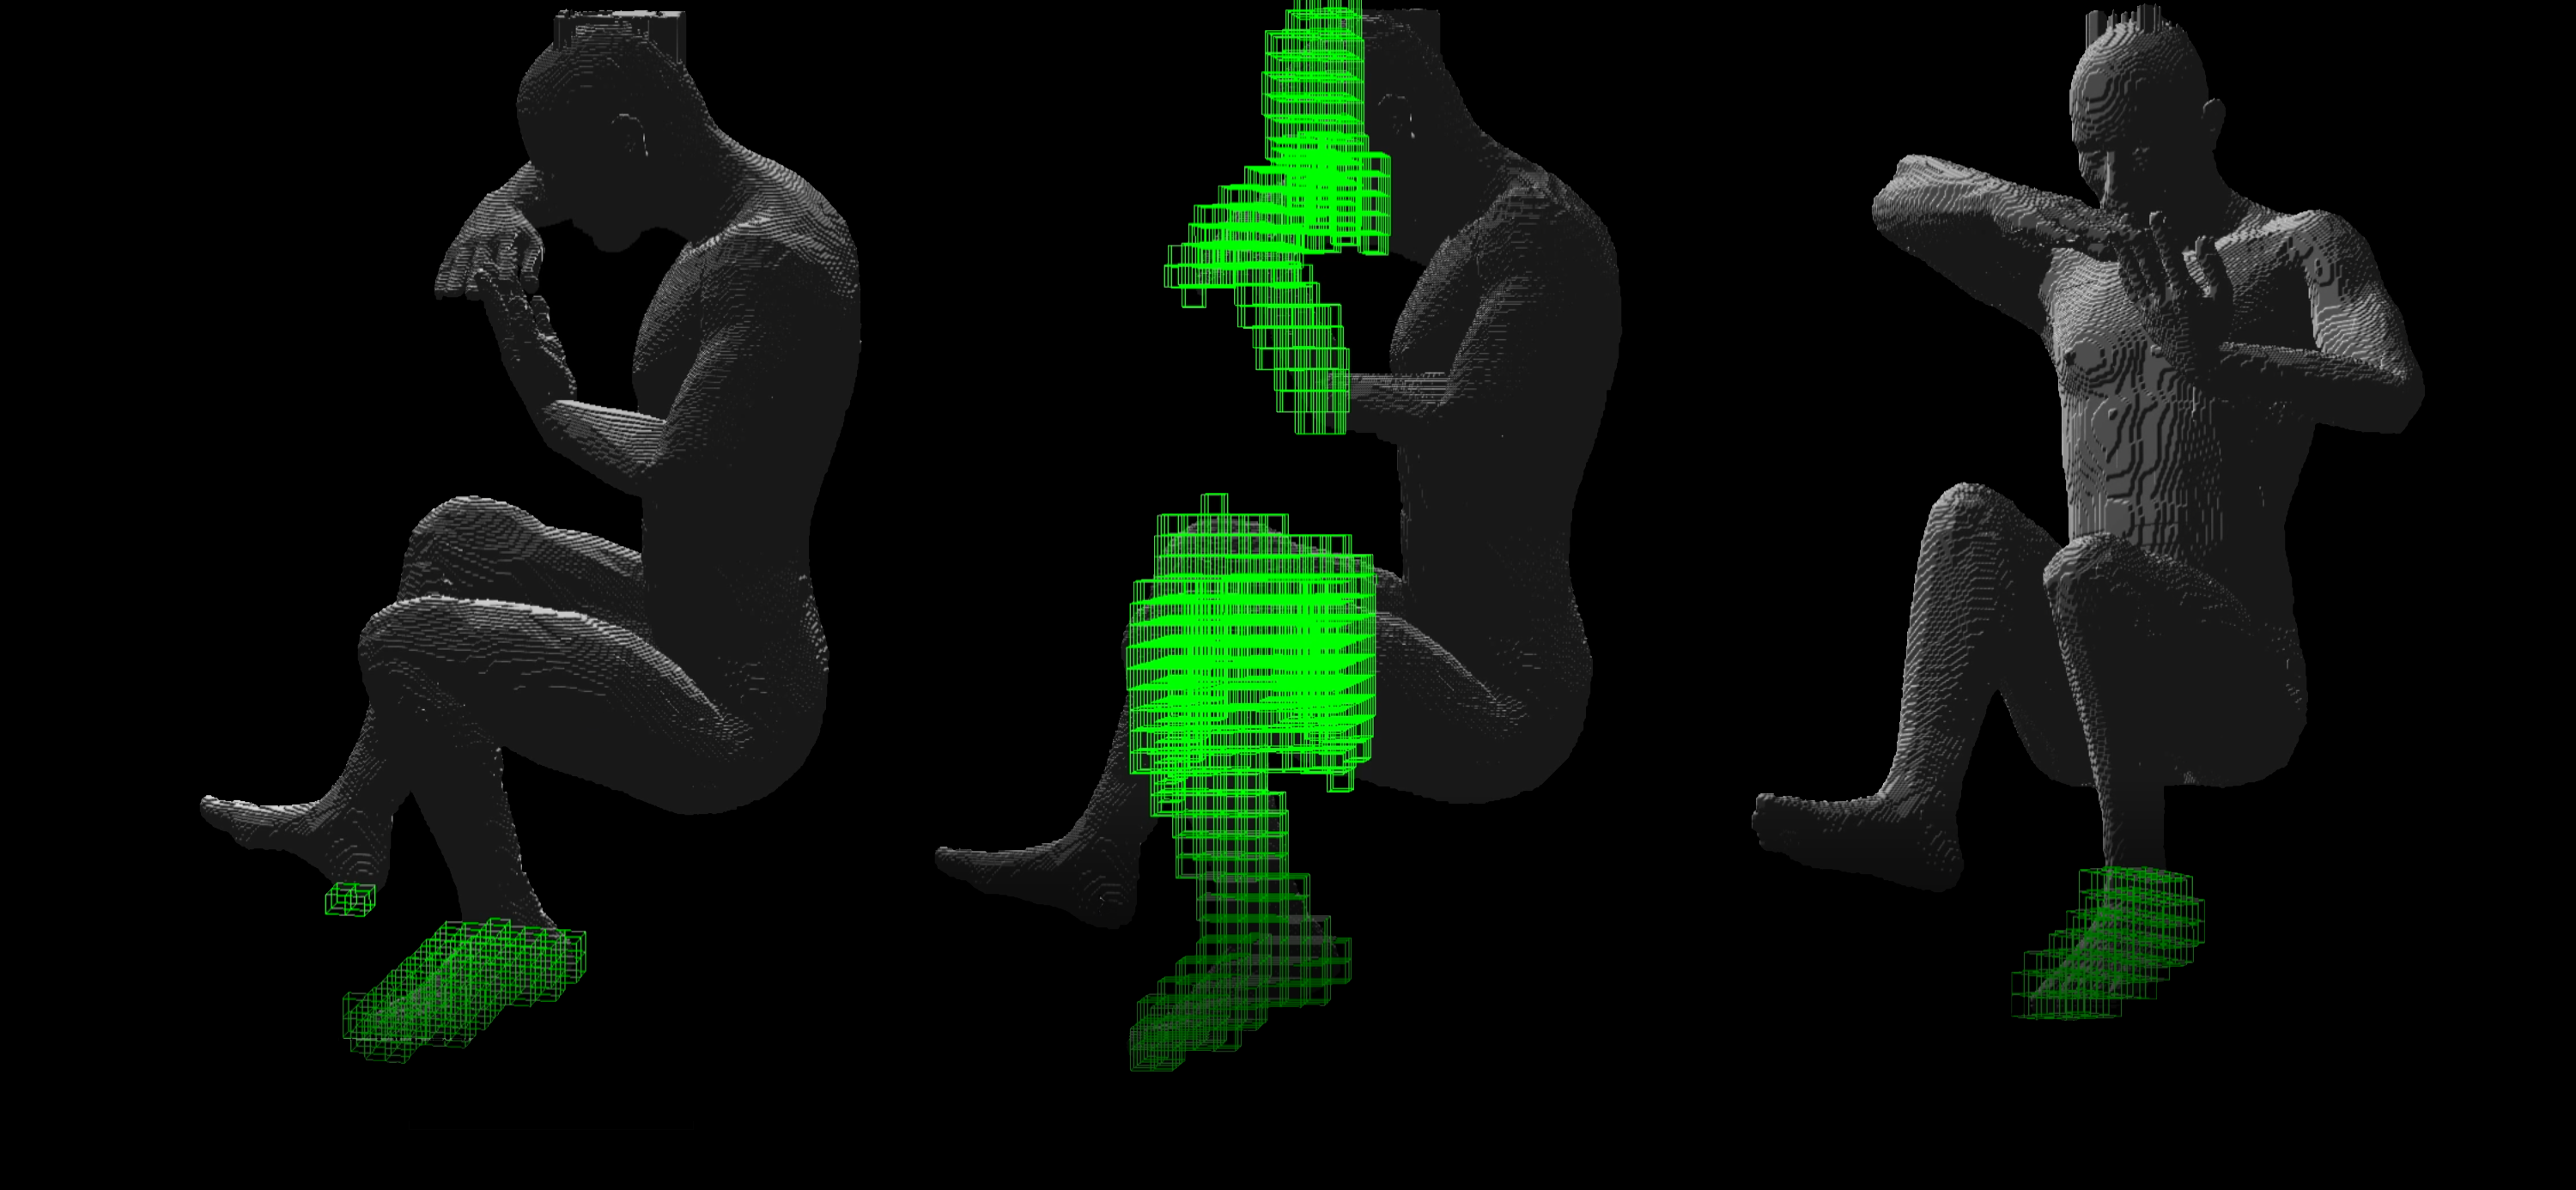
\includegraphics[width=14cm]{content/images/gvdb}
	\caption{The left and the middle image represent the selection process of the one keypoint in the data namely the left foot of the phantom. The right image shows the selected foot represented in green. The green boxes are a representation of the data on a higher level in the GVDB database.} 
	\label{fig:gvdb}
\end{figure}
\newpage
During the work on this master thesis different approaches have been tried to figure out how to automatically perform the rigging of the volumetric data. Unfortunately all approaches that have been tried did not deliver sufficient results. Although those attempts failed the results of them are stated in this section in order to explain and show what went wrong.

\subsection{Pinocchio}
The Pinocchio prototype introduced by Baran and Popovic is open source and available to download online \cite{Baran2007}. As stated in chapter \ref{ch:related} their approach need a watertight mesh as an input and will automatically calculate the armature which is somehow based on a predefined skeleton. In the paper about the automatic rigging and automation of \gls{3d} character the authors already mention that the discrete penalty functions used picture some assumptions which might lead to a unsatisfactory result when using their approach. Another downside of their algorithm is that it only works with mesh data and the data of fetal ultrasound investigations are normally given in voxel format. The transformation from the voxel data to a watertight mesh would lead to a loss of information and might not even be possible without human interaction. Although Shapiro et.al. introduced an algorithm based on the Pinocchio prototype which works with a voxel model as input. Unfortunately their implementation is not publicly available. The results when using the Pinocchio approach are depicted in Figure \ref{fig:PinocchioSkeleton}. The reason why this approach has not been progressed is that it seems that it will only work if the input data is somehow given in a standardized position.

\begin{figure} [!htb]
    \centering
	\includegraphics[width=7cm]{content/images/Pinocchio}
	\caption{Result of Pinocchio prototype applied to the man phantom model in its mesh representation.} 
	\label{fig:PinocchioSkeleton}
\end{figure}

\subsection{Skeletonization}
Another approach for the automatically rigging was to find a skeletonization representation of the data which may afterwards be mapped using joint mapping like introduced by Bharaj et.al. \cite{Bharaj2012}. This approach would need a curve skeleton as an input which perfectly represents the volume and is not somehow to complex. There are different approaches how to skeletonize a mesh but when working with voxels the selection is restricted. Altought two approaches have been tried. One is based on a Matlab toolbox called Volume Skeleton Toolbox. This toolbox provides different approaches for calculating the curve skeleton of volume data by thinning, distance field or potential field. When trying the approach with the distance matrix the result consisted of a huge amount of points. The potential field approach did not terminate and delivered a runtime exception and the thinning method somehow represented a skeleton but it was way to detailed. The result can be seen in Figure \ref{fig:skeleton}.\newline
It has also been tried to generate the Skeleton in MeVisLab using the $DtfSkeletonization$ module. The result of this approach is also depicted in Figure \ref{fig:skeleton}. It seams that there are some points of interest like the knee or other joints but it is also way to detailed and did not improve significantly when trying to use different settings in the module.

\begin{figure} [!htb]
    \centering
	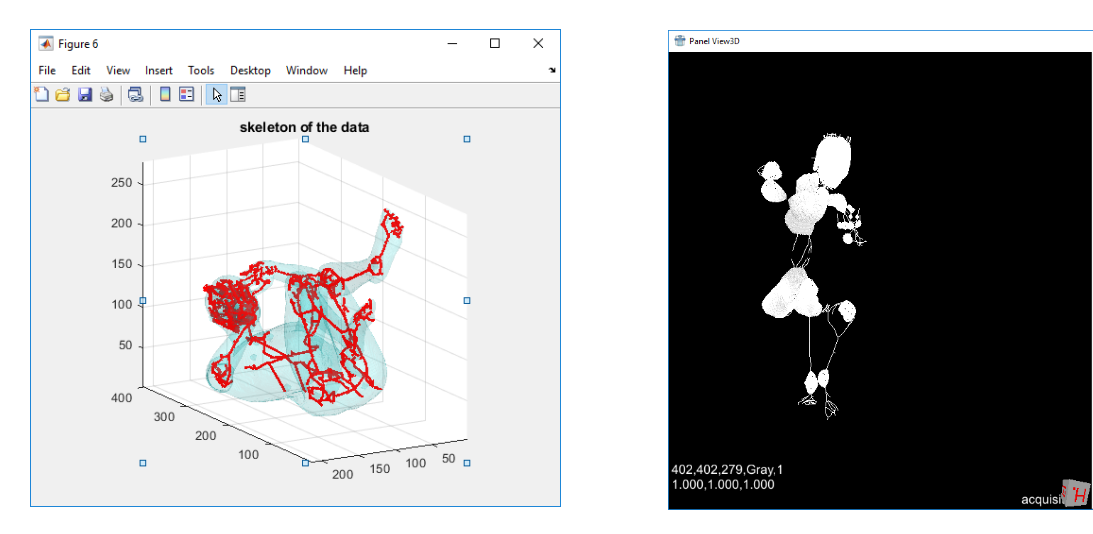
\includegraphics[width=15cm]{content/images/skeleton}
	\caption{The left image shows the skeletonization result when using the thinning option in the Matlab Volume Skeleton Toolbox and the image on the right hand side represents the skeleton as a result when using the $DtfSkeletonization$ module in MeVisLab.} 
	\label{fig:skeleton}
\end{figure}

\newpage
\section{Weighting of the data}
The weighting of the data is done by calculating the effect of each segment of the armature on the voxels surrounding the segments. For this processing step the Bender module $Volume Skinning$ is used. The module needs the original volume and the transformed armature as input and delivers an volume as output where the value of the voxels is set to the ID of the armature segments they belong to. The usage of this module is not intended to work with the data provided by the phantoms used in this thesis therefore unfortunately when using this module the option "Ignore Errors" has to be used. Normally the module would check if the armature is perfectly included in the volume and would not deliver an output if there are errors but this check does not work with the data provided here. Therefore the user has to be quite careful when using this module for the weighting process.\newline
There are also some alternative which may be used in order to calculate the weighting e.g. the geodesic distance based approach by Dionne and de Lasa \cite{Dionne2013GeodesicMeshes}. Their approach is also voxel based and would maybe deliver better results than the one used in Bender where unfortunately the authors doe not state which approach they use in order to calculate the weighting. In some cases like in the fetus phantom where the arms are quite stuck to the body the segments of the arm are in a conflict with the shoulders and the torso. In that case some artefacts might arise because the segments of the arms will have an influence on the voxels which should belong to the torso or to the shoulders. If such problems arise Bender also has a solution, namely the $Editor$ module where the user is able to override the weighting result. But one has to mention that this process can be very complex and time consuming because the editor only works in \gls{2d} and therefore each slice has to be adapted.

\begin{figure} [!htb]
    \centering
	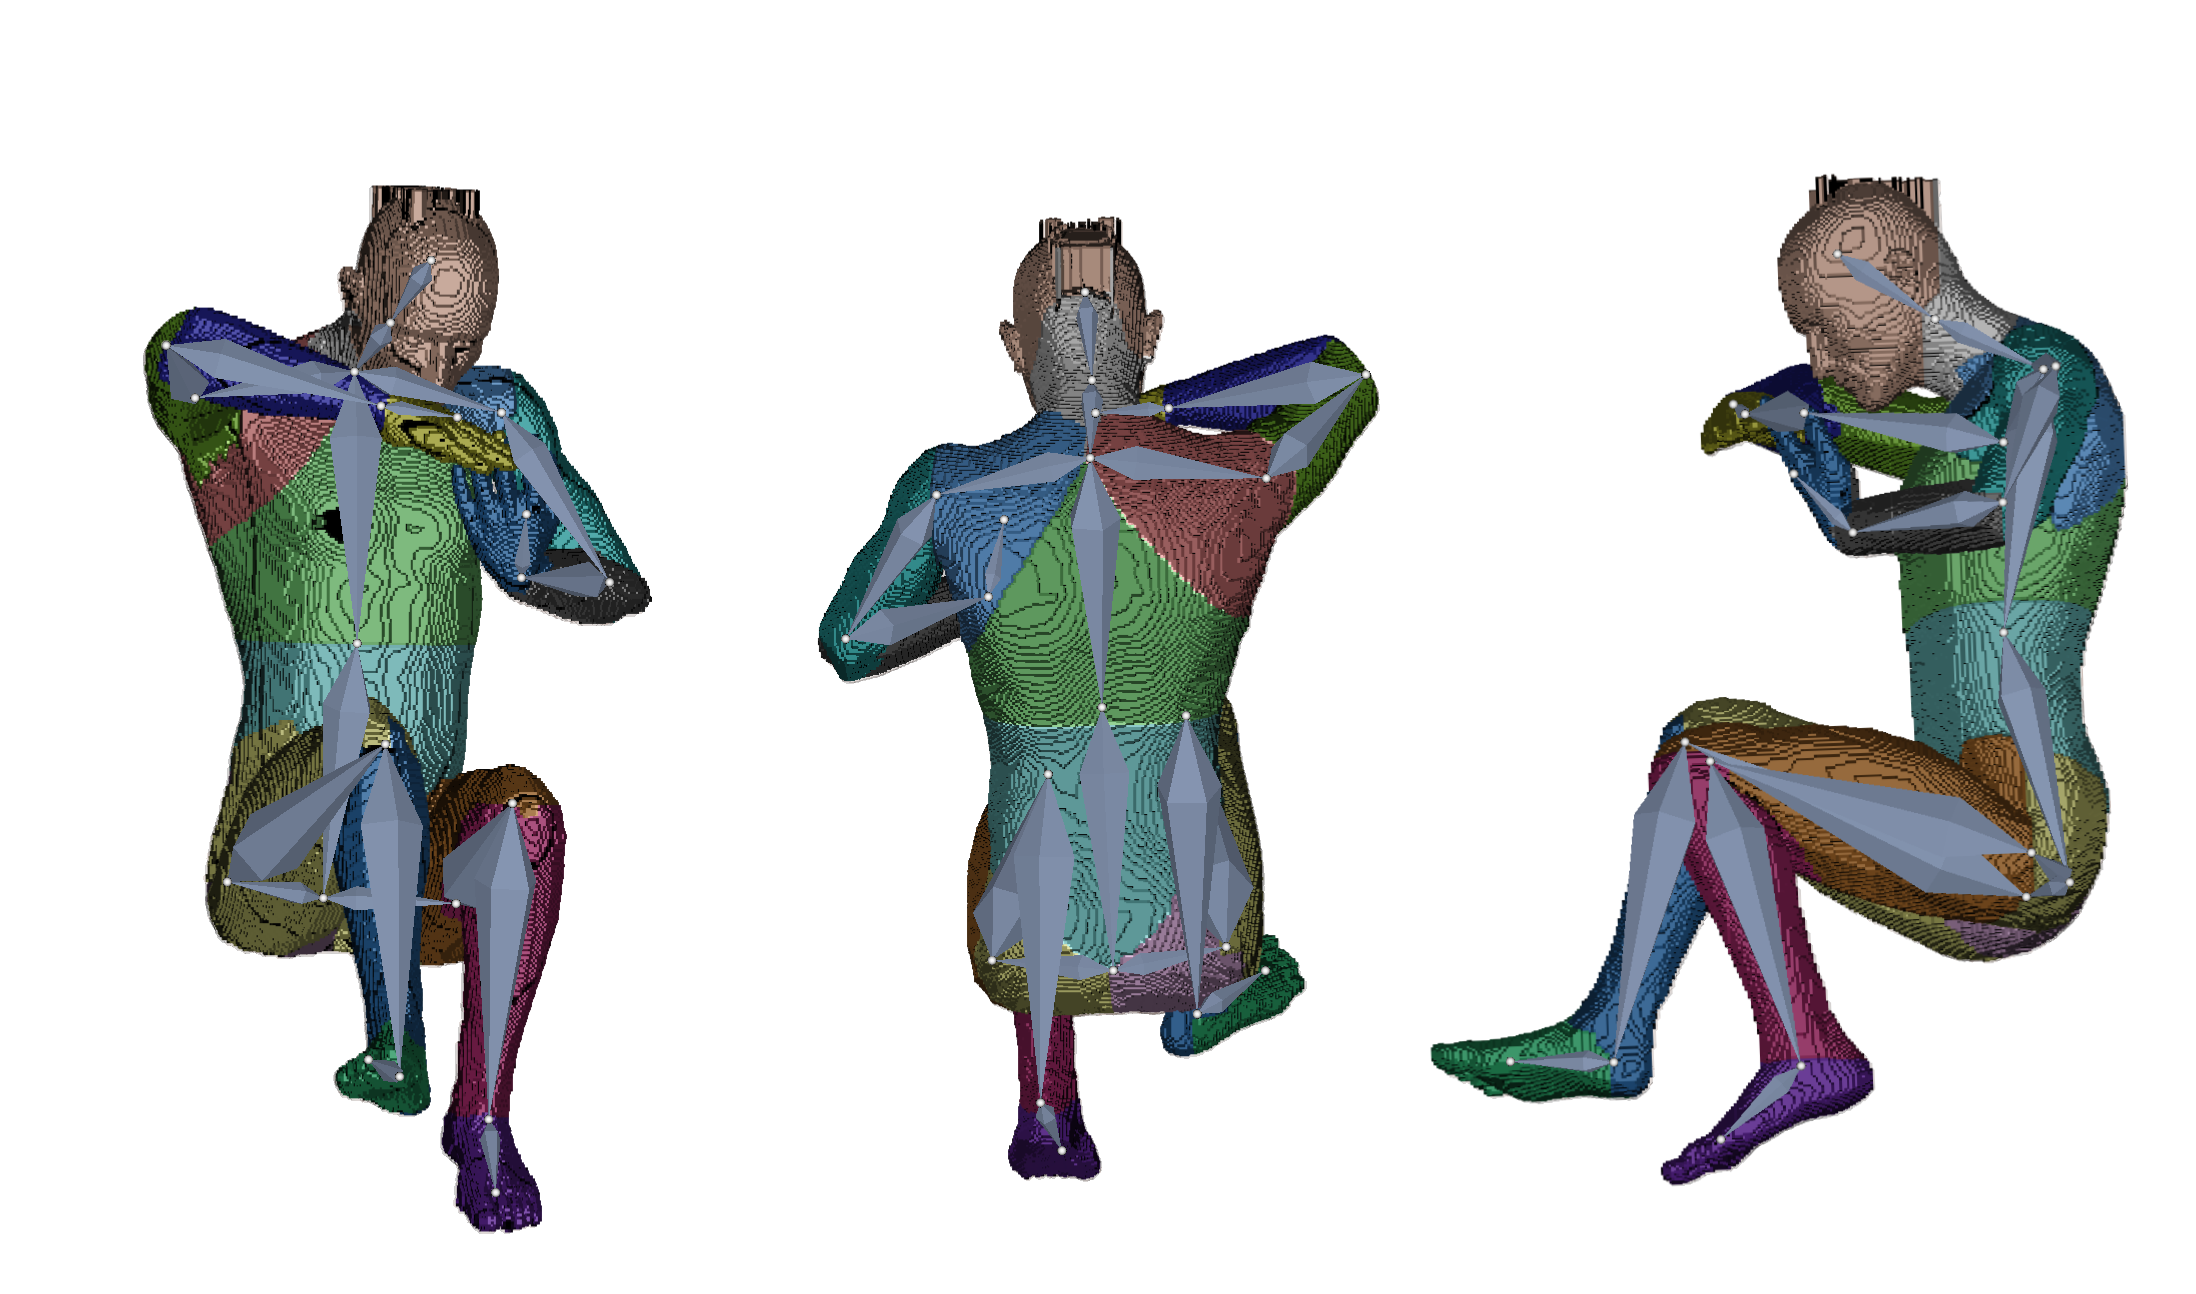
\includegraphics[width=12cm]{content/images/weight}
	\caption{Result of the weighting module in Bender. The colors represent the mapping to the according segments of the armature inside of the volume.} 
	\label{fig:weight}
\end{figure}


\newpage
\section{Transformation of the data}\label{sec:transformation}

The transformation of the data based on a model is the key feature introduced in this thesis. The transformation is done in 3D Slicer \cite{Slicer3DSlicer, Fedorov20123DNetwork} in an own extension with several modules that carry out the different operations needed in order to transform the data. The extension is portable and can be used for other purposes as well.

\subsection{Loading model and armature}

The first step of the processing in this module is to load the data as well as the armature. The armature is saved as *.vtk which is an own file format of the \gls{vtk}. It represents the armature as a graph which consists of several segments. Each segment is defined by an unique identifier and the segments are given by coordinates which state where the head and the tail of the segment is located in the coordinate system in \gls{3d}. The segments are always connected by their head except the first segment. The volumetric data is given in another file format namely *.mha which is a so called Meta Image. This file format is specified by the \gls{itk} and it contains the volumetric data. The input to this module is more specifically the output of the prior used Bender application which already includes the affiliation of the voxels to the segments of the armature by setting their value to the identifier of the segments of the armature. The data might be visualized using the $VolumeRendering$ module of the 3D slicer. Using it also reveals the mapping between the voxels and the amateur. A visualization of an example output may be seen in Figure \ref{fig:volumeRendering}.


\begin{figure} [!htb]
    \centering
	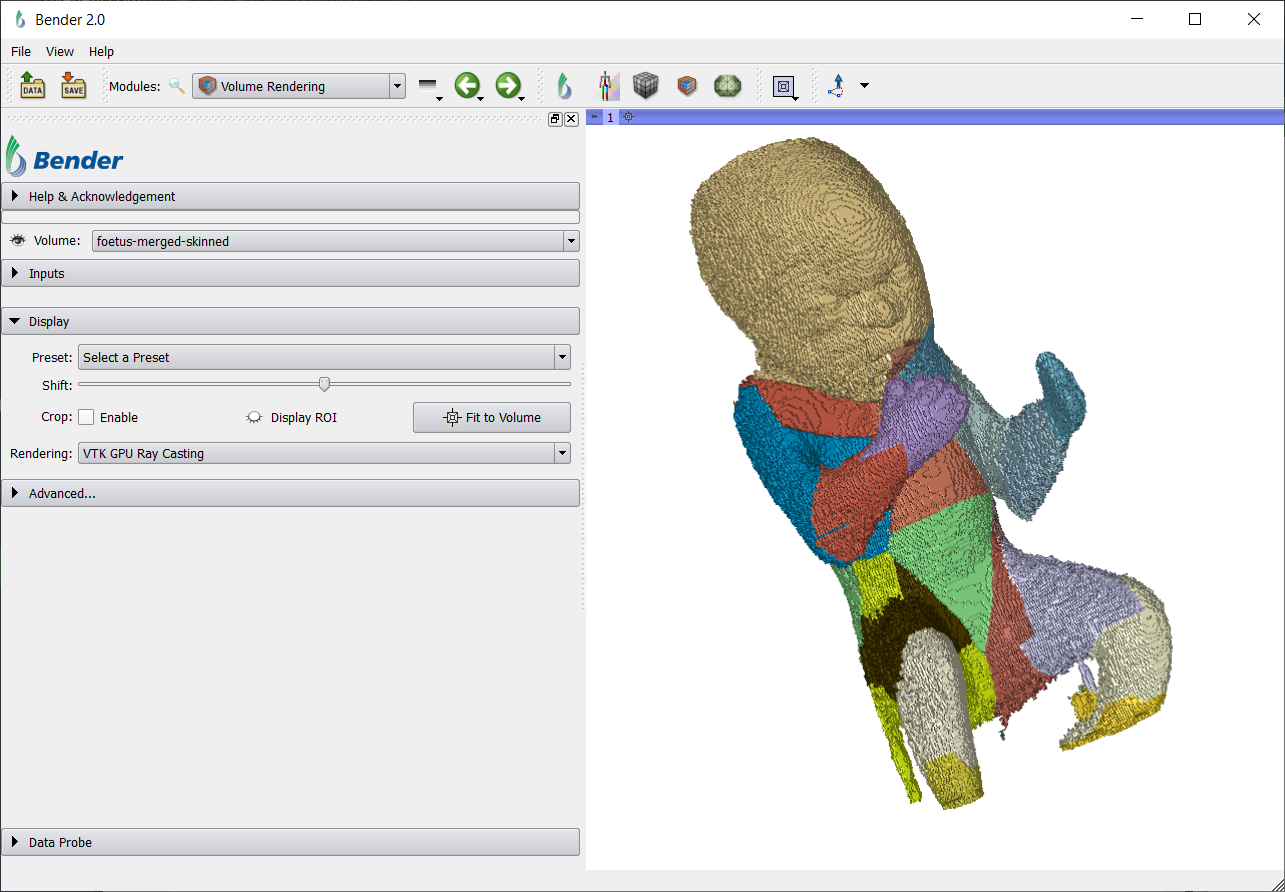
\includegraphics[width=8cm]{content/images/volumeRendering}
	\caption{Output of the $VolumeRendering$ module of 3D Slicer when visualizing the weighted fetus phantom model.} 
	\label{fig:volumeRendering}
\end{figure}


\newpage
\subsection{Calculate transform for each segment}

The basic idea of the approach is to transform each segment of the armature in respect to the segment attached or in some special cases like the transformation of the legs in respect to another segment which is not connected. The transformation that is needed is calculated by thinking of rotating the segment in a way, that it faces into the same direction then the segment before. In order to visualize this transformation process the left arm of a phantom is used. In this example the forearm of the left hand shall be transformed in a way that it faces in the same direction than the left upper arm. The left hand is just visualized in order to make the arm situation better perceivable. Of course the left arm also has to be transformed in order to align with the left forearm. The visualization of the initial pose is depicted in Figure \ref{fig:leftArm}.The legs are a somehow special case, because they should point in the same direction as the spine does and not as the abstraction of the pelvis does.

\begin{figure} [!htb]
    \centering
	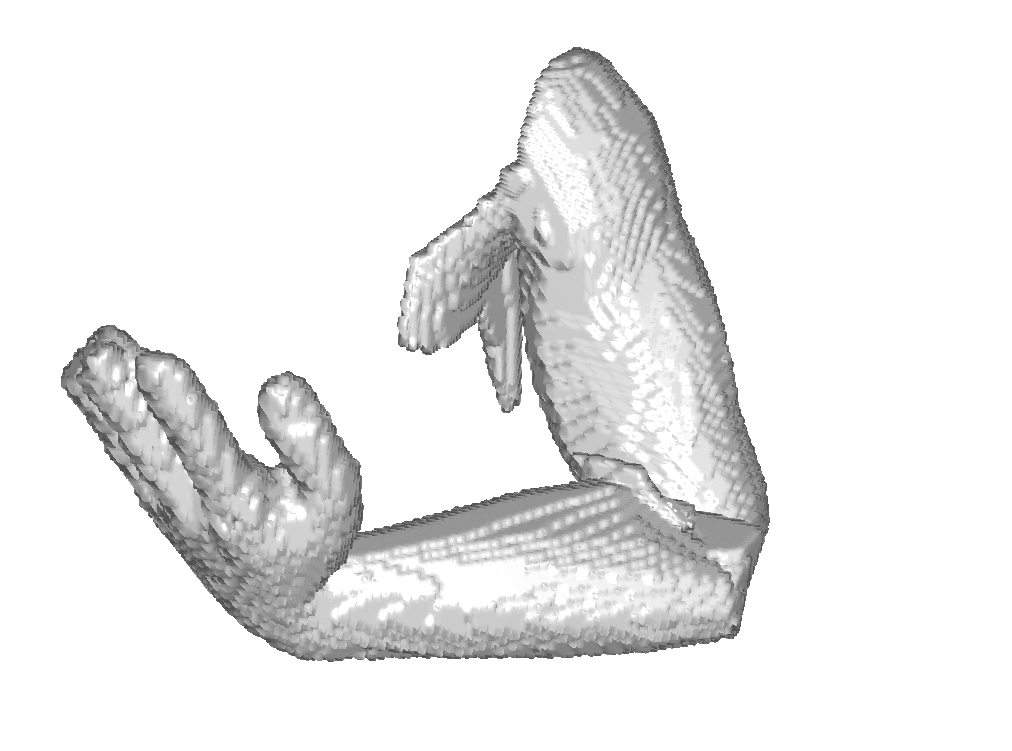
\includegraphics[width=10cm]{content/images/leftArm}
	\caption{Visualization of the initial pose of the left arm before transforming it.} 
	\label{fig:leftArm}
\end{figure}

In order to make the problem definition perceivable from a mathematical view the forearm is shifted to the head of the left upper arm. This represents a positioning of the coordinate system to the head of the left upper arm and shifting the left forearm to the origin of the new coordinate system. This does not have to be done in that way during the implementation it is only a way to visualize the methodical approach presented in this work.

\begin{figure} [!htb]
    \centering
	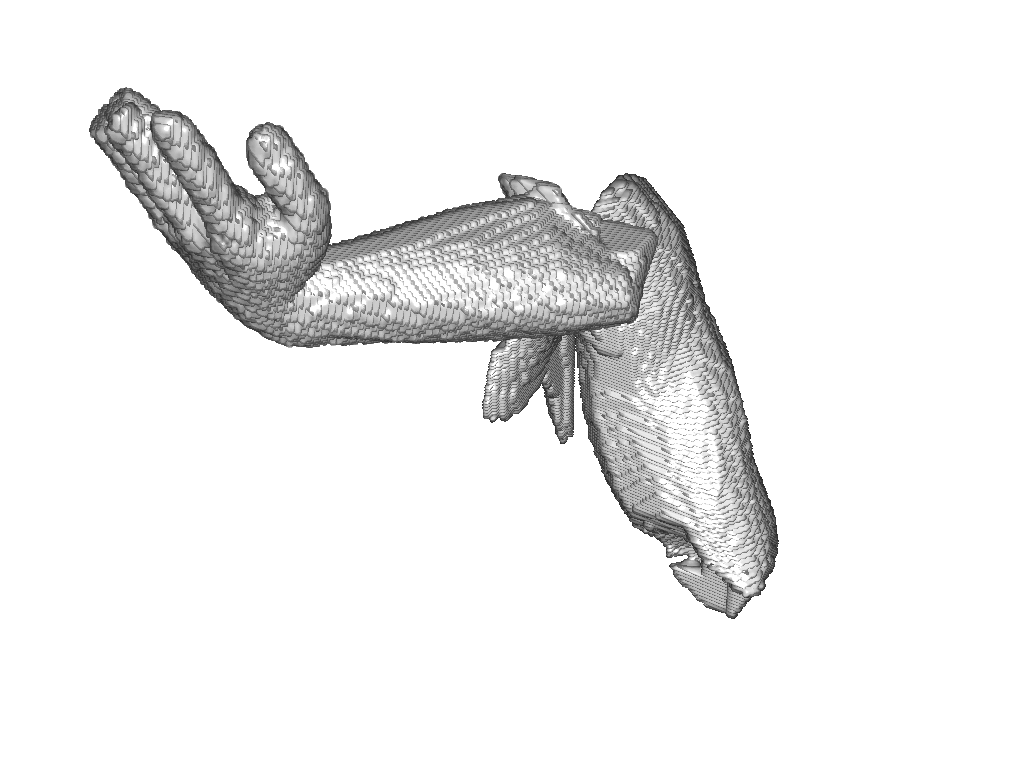
\includegraphics[width=10cm]{content/images/coordinateSystemShift}
	\caption{Image of the left forearm and hand shifted to the origin of the left upper arm in order to visualize the coordinate system shift.} 
	\label{fig:coordinateSystemShift}
\end{figure}

\newpage
\subsubsection{Mathematical basis}

For better understanding the problem is visualized as two vectors using Matlab. Figure \ref{fig:matlab} represents the output of the vector visualization. 

\begin{figure} [!htb]
    \centering
	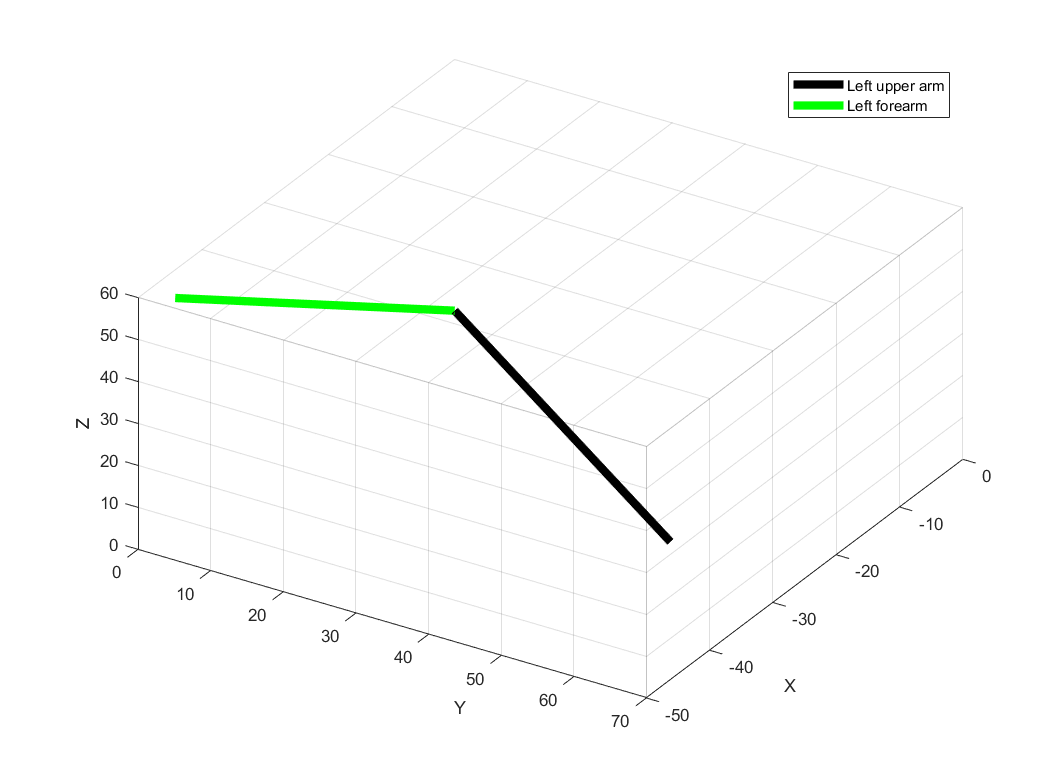
\includegraphics[width=10cm]{content/images/matlab.png}
	\caption{Vector representation of the left arm in Matlab, black being the left upper arm and green the left forearm.} 
	\label{fig:matlab}
\end{figure}

The result of the transformation for most of the segments should be that they face directly in the same direction. To do so two calculations have to be done. First an axis of rotation has to be found and second the angle between the two vectors. The angle of rotation is calculated by the Equation \ref{eq:axis} where u and v are the two vectors and a is the axis of rotation.

\begin{equation}
    a = u \times v / ||u \times v ||
    \caption{Axis of rotation between two vectors}
    \label{eq:axis}
\end{equation}

The angle between the vectors is calculated by Equation \ref{eq:angle}

\begin{equation}
    \alpha = arccos(u \cdot v)
    \caption{Angle between two vectors}
    \label{eq:angle}
\end{equation}

Having this information given one can easily calculate the rotation matrix about this arbitrary axis using the information provided my McDonald in his paper \cite{McdonaldAnimatedAxis}. Before representing the rotation matrix two further definitions have to be made, namely $c = cos(\alpha)$ and $s = sin(\alpha)$. The rotation matrix is presented in Equation \ref{eq:Rotation}.

\begin{equation}
    M_r = 
    \begin{bmatrix} 
    a_x^2(1-c)+c     & a_xa_y(1-c)-a_zs & a_xa_z(1-c)+a_ys \\
    a_xa_y(1-c)+a_zs & a_y^2(1-c)+c     & a_ya_z(1-c)-a_xs \\
    a_xa_z(1-c)-a_y  & a_ya_z(1-c)+a_xs & a_z^2(1-c)+c    
    \end{bmatrix} 
    \caption{Rotation matrix for rotation about an arbitrary axis \cite{McdonaldAnimatedAxis}.}
    \label{eq:RotationMatrix}
\end{equation}

McDonald states in his paper that it is important to have a as a unit vector because the matrix would not represent a rotation if it is not. The fact is that the rotation would be multiplied with the angle of rotation and therefore the result would not be the desired one. In Equation \ref{eq:Rotation} the result of the operation is shown in order to rotate a vector in the same direction than another one.

\begin{equation}
    v_r = M_ru
    \caption{Rotation of a vector in the direction of another vector by applying a rotation matrix about an arbitrary axis.}
    \label{eq:Rotation}
\end{equation}

Applying the rotation matrix to the given example the two vectors finally look like presented in the Figure \ref{fig:matlab2}.

\begin{figure} [!htb]
    \centering
	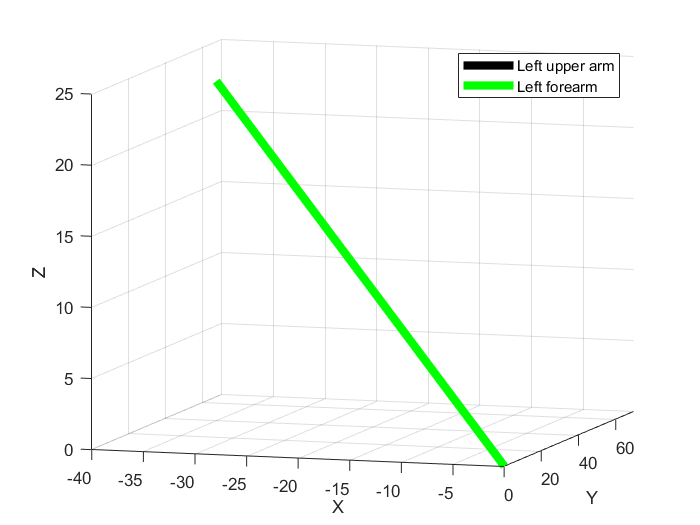
\includegraphics[width=10cm]{content/images/matlab2}
	\caption{Visualisation of the rotation result in Matlab. The black and the green vector representing the forearm and the upper arm are perfectly aligned.} 
	\label{fig:matlab2}
\end{figure}

The result in terms of data can be seen in Figure \ref{fig:leftArmOrRotation}. It represents the left forearm rotated in direction of the left upper arm. The whole rotation is then carried out without moving the forearm to the head of the upper arm. Instead the center of rotation is at the head of the forearm which is in fact the connection point between those two segments.The result of the rotation in that point is depicted in Figure \ref{fig:leftArmRRotation}.

\begin{figure} [!htb]
    \centering
	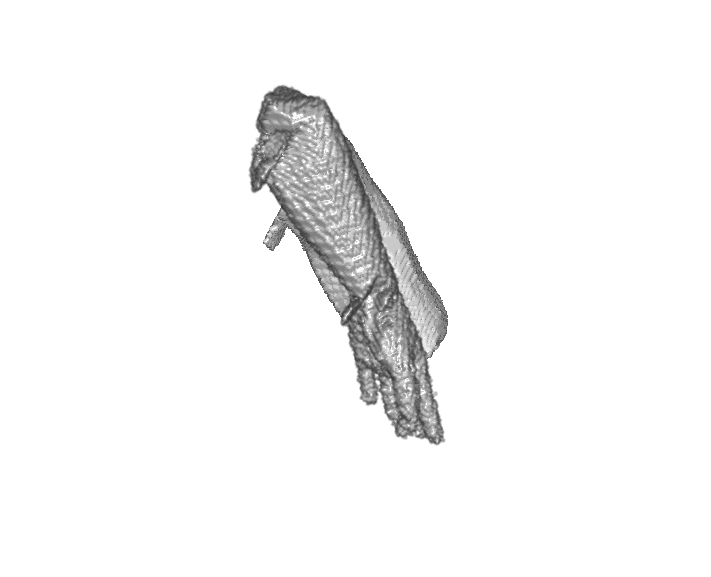
\includegraphics[width=10cm]{content/images/leftArmOrRotation.png}
	\caption{Result of the rotation of the left forearm with the center of rotation at the head of the left upper arm. Of course the left forearm has been moved to this point before.} 
	\label{fig:leftArmOrRotation}
\end{figure}
\begin{figure} [!htb]
    \centering
	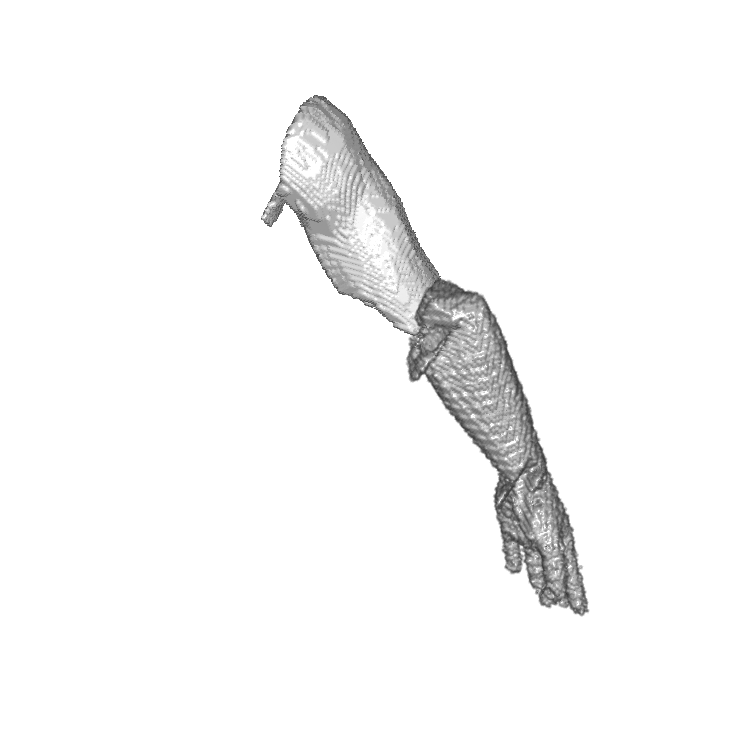
\includegraphics[width=10cm]{content/images/leftArmRRotation.png}
	\caption{Result of the rotation of the left forearm with the center of rotation at the connection point between left forearm and left upper arm.} 
	\label{fig:leftArmRRotation}
\end{figure}

\newpage
\subsection{Apply transform}

Having the rotation matrix defined which rotates one segment in the direction of the other segment the next step is to apply this transform to the voxels which belong to it. There is also one detail which should be kept in mind. The rotation matrix only describes the rotation around the arbitrary axis but the origin of the axis has to be set to be at the joint between two segments. This step may be performed by first shifting the segment of interest to the origin of the coordinate system, apply the transform there and shift it back. Or another possibility is to apply the transform considering a specific center of rotation. Some transformations are able to take such a center into account.

\newpage
\subsubsection{Integration in visualization framework}
In context of working with \gls{3d} visualization \gls{itk} is well known. Therefore we decided to work with it in terms of applying the transformation. The transformation is based on a given matrix and the center of rotation. Having both information the transformation is simply applied at the data using a $Resample$ filter. The filter takes the original image and the transformation an creates the output volume.\newline

\subsection{Save output}
The output of the method can be described as a volume which is a collection of volumes which represents the different parts of the armature. The volume can be saved as one file but the information about all the segments is also available. So for instance if one would like to examine the hand or the forearm of the fetus in greater detail there would also be the possibility to save those separately. In this work the save functionality of 3D Slicer is used which may be found in the Menu of the program. A screenshot of the program is depicted in Figure \ref{fig:saving}.


\begin{figure} [!htb]
    \centering
	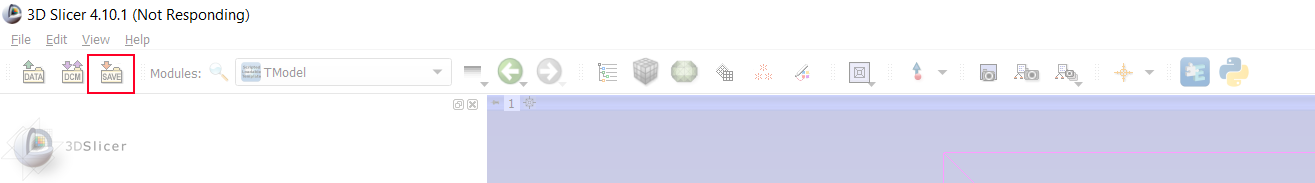
\includegraphics[width=12cm]{content/images/saving.png}
	\caption{Saving option in the menu of 3D Slicer.} 
	\label{fig:saving}
\end{figure}

\section{Analysis}
The analysis of data may be performed in many different ways. There could be of course some automatically performed analysis steps which may be performed on the generated output data. Those could for example calculate or display the range of the volumetric data in all three dimensions. This would then correlate to the crown toe distance and the spread of the arms. Normally one would measure these parameters by viewing at a \gls{2d} slice of the ultrasound like described in \ref{subsct:fetalGrowth}. Due to the fact that the method analysis and transforms each segment separately the volumetric information of each part is already given for analysis. So if it is needed there could be also volumetric statistics applied like how much volume does the head or some other parts of the body have. It can even be automatically compared if the volume of the right or the left limb is significantly higher. This would maybe the case in some growth disorders.

\newpage
In this work automatically analysis of the output data is not performed but there is a way to take measurements manually. 3D Slicer provides the user with a set of analysis tools like a ruler. The ruler can be applied in the 3D view and delivers the exact distance between two points. If the ruler is applied at the crown and the toe it will deliver the crown toe distance. Another more common distance would be the crown rump measurement. In Figure \ref{fig:ruler} the ruler can be seen in the toolbar and in Figure \ref{fig:rulerResult} the visualization in the 3D view of Slicer is shown. The ruling is performed interactively and can be adapted in the \gls{3d} view.\newline


\begin{figure} [!htb]
    \centering
	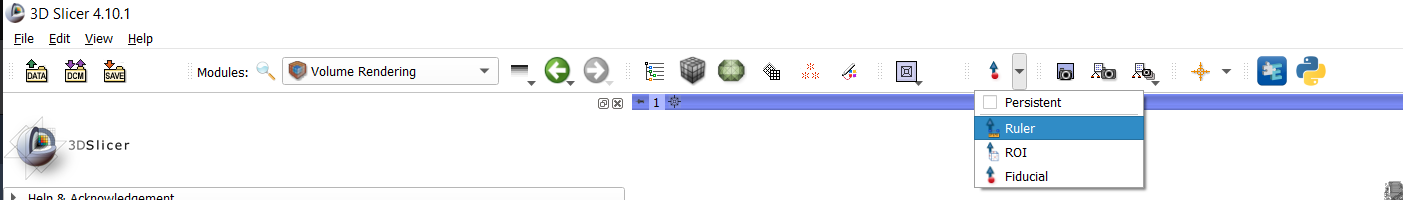
\includegraphics[width=14cm]{content/images/ruler.png}
	\caption{Ruler option in the 3D Slicer menu.} 
	\label{fig:ruler}
\end{figure}

\begin{figure} [!htb]
    \centering
	\includegraphics[width=16cm]{content/images/rulerResult.png}
	\caption{Result of two ruler operations on the T transformed model measuring the crown toe length and the spread of the arms.} 
	\label{fig:rulerResult}
\end{figure}
\newpage

\chapter{Implementation}
\section{Implementation overview}

\section{Slicer module and extension}

\section{Thresholding volume}

\section{Transforming data according to armature}

\section{Adding scalar volume}

\section{Input and output data}
\newpage

\chapter{Results}\label{ch:result}
The approach shown in this thesis has been tested using different types of input data. One of the most interesting outcomes when testing new algorithms methods or approaches is to try to express the performance in terms of values and absolute values. That is why we decided to test the method with a phantom dataset of a man, which has been gathered from the internet \cite{Squidifier2010DetailedMan}. The model is already in a T-pose and therefore the example of how the output should look like. The model is adapted in Blender in order to bring it into different poses which reflect natural poses of fetus in the belly. The input dataset is shown in Figure \ref{fig:tPose}.

\begin{figure} [htb!]
    \centering
	\includegraphics[width=11cm]{content/images/results/TPosition.png}
	\caption{The initial pose of the phantom data used to evaluate the method against the standardized position \cite{Squidifier2010DetailedMan}.}
	\label{fig:tPose}
\end{figure}

The first part of the result section is mainly about the performance of algorithm on the presented phantom of a man. The structure will be that first the initial pose and the armature in the data will be presented and afterwards the final T-pose of the data which is the output of the method applied. Then there is a section which handles the fetus data which is unfortunately also phantom data. The second major part of this chapter is about an influence analysis where results are presented which did not perform well and represent the effects of different influences in the given input data.

\newpage
\section{Performance of the algorithm}

\begin{figure} [htb!]
    \centering
	\includegraphics[width=13cm]{content/images/results/man1Front.png}
	\caption{Front view of the first fetus pose. On the left the volume visualization of the prototype and on the right the visualization of the included armature.}
	\label{fig:}
\end{figure}
\begin{figure} [htb!]
    \centering
	\includegraphics[width=13cm]{content/images/results/man1Top.png}
	\caption{Top view of the same formation also volume and armature view.}
	\label{fig:}
\end{figure}

\begin{figure} [htb!]
    \centering
	\includegraphics[width=15cm]{content/images/results/man1Side.png}
	\caption{Side view of the pose also with visible armature and volume visualization.}
	\label{fig:}
\end{figure}

\vspace*{2cm}

\begin{figure} [htb!]
    \centering
	\includegraphics[width=16cm]{content/images/results/man1Result.png}
	\caption{The result T-pose of the first fetus pose from left to right: Top view, front view and side view.}
	\label{fig:}
\end{figure}
%% START MAN 2
\newpage
\begin{figure} [htb!]
    \centering
	\includegraphics[width=13cm]{content/images/results/man2Front.png}
	\caption{Front view of the second fetus pose. On the left the volume visualization of the prototype and on the right the visualization of the included armature.}
	\label{fig:}
\end{figure}
\begin{figure} [htb!]
    \centering
	\includegraphics[width=13cm]{content/images/results/man2Top.png}
	\caption{Top view of the same formation also volume and armature view.}
	\label{fig:}
\end{figure}

\begin{figure} [htb!]
    \centering
	\includegraphics[width=15cm]{content/images/results/man2Side.png}
	\caption{Side view of the pose also with visible armature and volume visualization.}
	\label{fig:}
\end{figure}
\vspace*{3cm}
\begin{figure} [htb!]
    \centering
	\includegraphics[width=15cm]{content/images/results/man2Result.png}
	\caption{The result T-pose of the second fetus pose from left to right: Top view, front view and side view.}
	\label{fig:}
\end{figure}
\newpage
%% START MEN 3
\begin{figure} [htb!]
    \centering
	\includegraphics[width=13cm]{content/images/results/man3Front.png}
	\caption{Front view of the third fetus pose. On the left the volume visualization of the prototype and on the right the visualization of the included armature.}
	\label{fig:}
\end{figure}
\begin{figure} [htb!]
    \centering
	\includegraphics[width=13cm]{content/images/results/man3Top.png}
	\caption{Top view of the same formation also volume and armature view.}
	\label{fig:}
\end{figure}

\begin{figure} [htb!]
    \centering
	\includegraphics[width=15cm]{content/images/results/man3Side.png}
	\caption{Side view of the pose also with visible armature and volume visualization.}
	\label{fig:}
\end{figure}

\vspace{3cm}

\begin{figure} [htb!]
    \centering
	\includegraphics[width=15cm]{content/images/results/man3Result.png}
	\caption{The result T-pose of the third fetus pose from left to right: Top view, front view and side view.}
	\label{fig:}
\end{figure}
%% START MAN 4
\newpage
\begin{figure} [htb!]
    \centering
	\includegraphics[width=13cm]{content/images/results/man4Front.png}
	\caption{Front view of the fourth fetus pose. On the left the volume visualization of the prototype and on the right the visualization of the included armature.}
	\label{fig:}
\end{figure}
\begin{figure} [htb!]
    \centering
	\includegraphics[width=13cm]{content/images/results/man4Top.png}
	\caption{Top view of the same formation also volume and armature view.}
	\label{fig:}
\end{figure}

\begin{figure} [htb!]
    \centering
	\includegraphics[width=15cm]{content/images/results/man4Side.png}
	\caption{Side view of the pose also with visible armature and volume visualization.}
	\label{fig:}
\end{figure}
\vspace*{3cm}
\begin{figure} [htb!]
    \centering
	\includegraphics[width=16cm]{content/images/results/man4Result.png}
	\caption{The result T-pose of the fourth fetus pose from left to right: Top view, front view and side view.}
	\label{fig:}
\end{figure}
%% START MAN 5
\newpage
\begin{figure} [htb!]
    \centering
	\includegraphics[width=13cm]{content/images/results/man5Front.png}
	\caption{Front view of the fifth fetus pose. On the left the volume visualization of the prototype and on the right the visualization of the included armature.}
	\label{fig:}
\end{figure}
\begin{figure} [htb!]
    \centering
	\includegraphics[width=13cm]{content/images/results/man5Top.png}
	\caption{Top view of the same formation also volume and armature view.}
	\label{fig:}
\end{figure}

\begin{figure} [htb!]
    \centering
	\includegraphics[width=15cm]{content/images/results/man5Side.png}
	\caption{Side view of the pose also with visible armature and volume visualization.}
	\label{fig:}
\end{figure}
\vspace{3cm}
\begin{figure} [htb!]
    \centering
	\includegraphics[width=16cm]{content/images/results/man5Result.png}
	\caption{The result T-pose of the fifth fetus pose from left to right: Top view, front view and side view.}
	\label{fig:}
\end{figure}

%% START MAN 6
\newpage
\begin{figure} [htb!]
    \centering
	\includegraphics[width=13cm]{content/images/results/man6Front.png}
	\caption{Front view of the sisxth fetus pose. On the left the volume visualization of the prototype and on the right the visualization of the included armature.}
	\label{fig:}
\end{figure}
\begin{figure} [htb!]
    \centering
	\includegraphics[width=13cm]{content/images/results/man6Top.png}
	\caption{Top view of the same formation also volume and armature view.}
	\label{fig:}
\end{figure}

\begin{figure} [htb!]
    \centering
	\includegraphics[width=15cm]{content/images/results/man6Side.png}
	\caption{Side view of the pose also with visible armature and volume visualization.}
	\label{fig:}
\end{figure}
\vspace{3cm}
\begin{figure} [htb!]
    \centering
	\includegraphics[width=16cm]{content/images/results/man6Result.png}
	\caption{The result T-pose of the sixth fetus pose from left to right: Top view, front view and side view.}
	\label{fig:}
\end{figure}

%% START MAN 7
\newpage
\begin{figure} [htb!]
    \centering
	\includegraphics[width=13cm]{content/images/results/man7Front.png}
	\caption{Front view of the seventh fetus pose. On the left the volume visualization of the prototype and on the right the visualization of the included armature.}
	\label{fig:}
\end{figure}
\begin{figure} [htb!]
    \centering
	\includegraphics[width=13cm]{content/images/results/man7Top.png}
	\caption{Top view of the same formation also volume and armature view.}
	\label{fig:}
\end{figure}

\begin{figure} [htb!]
    \centering
	\includegraphics[width=15cm]{content/images/results/man7Side.png}
	\caption{Side view of the pose also with visible armature and volume visualization.}
	\label{fig:}
\end{figure}
\vspace{3cm}
\begin{figure} [htb!]
    \centering
	\includegraphics[width=16cm]{content/images/results/man7Results.png}
	\caption{The result T-pose of the seventh fetus pose from left to right: Top view, front view and side view.}
	\label{fig:}
\end{figure}

\clearpage
\subsubsection{Performance statistics}
As stated in the begin of this chapter performance analysis is importing when presenting a novel method or approach and therefore we tried to measure how good the algorithm performs. The performance is measured using different operations. First there is a time consuming part involved in the process of having the T-pose transformed data namely the rigging, described in \ref{sct:rigging}. Therefore the time being spent in the program Blender \cite{Foundation2019Blender} has been measured from the step of loading the data until the result has been saved for further processing. The overview of the times is shown in Table \ref{tbl:duration}. The average duration of the whole process being done in Blender is \textbf{seven} Minutes. The rigging is performed by the author and therefore maybe someone less familiar would perform slower. 

\begin{table}[!htb]
    \centering
    \begin{tabular}{l|l|l|l}
    Phantom & Starting time & End time & Duration \\ \hline
    Man1    & 15:12         & 15:24    & 00:12    \\ \hline
    Man2    & 16:46         & 16:50    & 00:04    \\ \hline
    Man3    & 15:41         & 15:52    & 00:11    \\ \hline
    Man4    & 16:12         & 16:21    & 00:09    \\ \hline
    Man5    & 16:24         & 16:30    & 00:06    \\ \hline
    Man6    & 16:32         & 16:36    & 00:04    \\ \hline
    Man7    & 16:38         & 16:44    & 00:06   
    \end{tabular}
    \caption{Overview of the duration needed to rig the seven phantom models.}
    \label{tbl:duration}
\end{table}

The second and maybe most important measurement of performance is how well the transformed data represent the original T-pose. Therefore the result has been registered with the T-pose input and the scalar volume difference has been produced. The result of one of those measurements is shown in Figure \ref{fig:differences}. It somehow looks like that there is lots of data left and therefore the overlapping is low, but it has to be considered that the data is volumetric and therefore the number of voxels remaining is important and not if the rest still looks like a human. The analysis results are presented in Table \ref{tbl:performance}. The average of the overlap percentage is \textbf{}{79,02\%} which depends on how well the armature is placed in the data.
 
\begin{figure} [htb!]
	\includegraphics[width=14cm]{content/images/results/man4Differences}
	\caption{The result of the difference of the fourth fetus pose from left to right: Top view, front view and side view.}
	\label{fig:differences}
\end{figure}

\begin{table}[!htb]
    \centering
    \begin{tabular}{l|l|l|l}
    \begin{tabular}[c]{@{}l@{}}Total amount\\ voxels T-pose\end{tabular} & \begin{tabular}[c]{@{}l@{}}Amount of voxels\end{tabular}\\\begin{tabular}[c]{@{}l@{}}Percentage of voxels\\left after subtraction\end{tabular} & Percentage Left & Percentage Overlap \\ \hline
    2654642 & 790637 & 29,78\% & 70,22\% \\ \hline
    2654642 & 886471 & 33,39\% & 66,61\% \\ \hline
    2654642 & 572079 & 21,55\% & 78,45\% \\ \hline
    2654642 & 530825 & 20,00\% & 80,00\% \\ \hline
    2654642 & 492437 & 18,55\% & 81,45\% \\ \hline
    2654642 & 286991 & 10,81\% & 89,19\% \\ \hline
    2654642 & 338764 & 12,76\% & 87,24\%           
    \end{tabular}
    \caption{The table shows the total amount of voxels in the T-pose and the amount of voxels left after subtraction of the result of the method and the T-pose. The left two columns }
    \label{tbl:performance}
\end{table}

\clearpage
\subsection{Fetus data}
The fetus data presented in this section is also gathered from the internet. One dataset is a simple \gls{3d} model of a fetus \cite{SpecialboyBebyModel} and the other one a simulation of a whole fetus ultrasound scan produced by Cortes et.al. \cite{Cortes2016UltrasoundEvaluation}. This section is structured just as the one with the man phantoms. The difference between the datasets is that in this case there is no ground truth that can be compared so there is no T-pose which is the right solution. Therefore the only performance analysis can be done in terms of time needed for rigging the data.

\begin{figure} [htb!]
    \centering
	\includegraphics[width=11cm]{content/images/results/fetusModelFront.png}
	\caption{Front view of the fetus model \cite{SpecialboyBebyModel}. On the left the volume visualization of the prototype and on the right the visualization of the included armature.}
	\label{fig:}
\end{figure}
\begin{figure} [htb!]
    \centering
	\includegraphics[width=13cm]{content/images/results/fetusModelTop.png}
	\caption{Top view of it also volume and armature view.}
	\label{fig:}
\end{figure}
\begin{figure} [htb!]
    \centering
	\includegraphics[width=14cm]{content/images/results/fetusModelSide.png}
	\caption{Side view of the pose also with visible armature and volume visualization.}
	\label{fig:}
\end{figure}
\begin{figure} [htb!]
    \centering
	\includegraphics[width=14cm]{content/images/results/fetusModelResult.png}
	\caption{The result T-pose of the fetus model from left to right: Top view, front view and side view.}
	\label{fig:}
\end{figure}
\newpage

The following data shows the phantom model which represents how the output of a full fetus ultrasound scan may look like. The data has been pre-filtered in order to make is usable for the method presented. The original data is shown in Figure \ref{fig:phantomFetusOriginalData}.

\begin{figure} [htb!]
    \centering
	\includegraphics[width=8cm]{content/images/phantomFetusOr.PNG}
	\caption{Original phantom model created by Cortes \cite{Cortes2016UltrasoundEvaluation} which represents a phanom of a full fetus \gls{3d} ultrasound scan.}
	\label{fig:phantomFetusOriginalData}
\end{figure}

The result of the preprocessing step and the result of the fetus formation is shown here.
\begin{figure} [htb!]
    \centering
	\includegraphics[width=13cm]{content/images/results/fetusPhantomFront.png}
	\caption{Front view of the fetus phantom provided by Cortes \cite{Cortes2016UltrasoundEvaluation}. On the left the volume visualization of the prototype and on the right the visualization of the included armature.}
	\label{fig:}
\end{figure}
\begin{figure} [htb!]
    \centering
	\includegraphics[width=13cm]{content/images/results/fetusPhantomTop.png}
	\caption{Top view of the phantom also volume and armature view.}
	\label{fig:}
\end{figure}
\begin{figure} [htb!]
    \centering
	\includegraphics[width=15cm]{content/images/results/fetusPhantomSide.png}
	\caption{Side view of the pose also with visible armature and volume visualization.}
	\label{fig:}
\end{figure}
\begin{figure} [htb!]
    \centering
	\includegraphics[width=16cm]{content/images/results/fetusPhantumResult.png}
	\caption{The result T-pose of the fetus phantom from left to right: Top view, front view and side view.}
	\label{fig:}
\end{figure}

\clearpage
The analysis of the method in terms of fetus like or phantom fetus model is represented by the time the end user needs in order to perform the manual step of rigging. Table \ref{tbl:fetusPerformance} represents the time needed to perform this manual step. The average time to do so is \textbf{eight} minutes.

\begin{table}[!htb]
    \centering
    \begin{tabular}{l|l|l|l}
                   & Starting time & End time & Duration \\\hline
    Fetus Model     & 18:50         & 18:56    & 00:06    \\\hline
    Fetus US Phantom & 19:00         & 19:11    & 00:11   
    \end{tabular}
    \label{tbl:fetusPerformance}
    \caption{Table representing the time needed for rigging the fetus model and the fetus ultrasound phantom.}
\end{table}

\section{Influence analysis}
This section of the results handles findings which somehow show where the limits of the method are. There are some influences which lead to major artefacts and unwanted results. Those like limiting cases are  presented here.

\subsection{Noise}

The first problem which has been identified is the influence of noise in the data. In case of the phantom ultrasound investigation result created by Cortes et.al. \cite{Cortes2016UltrasoundEvaluation} noise which is usual for an ultrasound investigation has been added. If this data is directly loaded into the blender application the result looks like shown in Figure \ref{fig:noiseVies} and Figure \ref{fig:noise3D}. This data cannot be used in order to rig the data and produce meaningful output. Therefore the preprocessing step has been established. The surrounding of the data has to be free of any noise. In fact the data representing the fetus itself may have some noise included which can be seen in the results of the fetus phantom.

\begin{figure} [htb!]
    \centering
	\includegraphics[width=13cm]{content/images/influence/viewsNoise.png}
	\caption{Different views of the noise in the phantom ultrasound data provided by Cortes et.al. \cite{Cortes2016UltrasoundEvaluation} in Bender \cite{Finet2014Bender:Morphing}.}
	\label{fig:noiseVies}
\end{figure}

\begin{figure} [htb!]
    \centering
	\includegraphics[width=13cm]{content/images/influence/noise3D.png}
	\caption{\gls{3d} visualisation of the fetus phantom with the noise included in Bender \cite{Finet2014Bender:Morphing}.}
	\label{fig:noise3D}
\end{figure}


\subsection{Weighting issues}

In some cases especially when the pose of the fetus is really packed and the limbs are very close to the body the weighting of the data does not perform very well. The problem is that if the arms are connected with the body the armature in the arms will compete with the armature in the body, namely the torso and the belly. The voxels in between those armature will be divided and the armature in the upper part will get a piece of the body which should not happen. Another example is given when the tighs are very close to he body they will somehow share some parts of the belly or of the pelvis. This phenomena is also likely to occur if the arms touch the legs. One example of this weighting issue is presented in Figure \ref{fig:weightingissue}.

\begin{figure} [htb!]
    \centering
	\includegraphics[width=9cm]{content/images/results/weightingIssues.png}
	\caption{Visualization of the weighting of the fetus phantom model. The arms and the legs have too much voxels assigned to them.}
	\label{fig:weightingissue}
\end{figure}

\newpage
\subsection{Limited space for rotation}

Another issue which has been faced during the evaluation phase was that the size of the volume to be worked with is somehow limited. The male phantom models have a resolution of 402x402 and around 250 in the depth which depends on the pose of the model. In order to perform all the rotations without limbs getting cut off by the volume borders first the volume is expanded by a factor of two which results in a volume size of around 800 times 800 and 500 in the depth. This is somehow also the limitation for the $threshold$ function in 3D Slicer. In some cases like the examples five, six and seven the expanding of the volume to the doubled size has not been enough. The initial result may be seen in Figure \ref{fig:rotationProblem}. If such datasets have to be analysed they have to be scaled down before they can be used. The scaling is done in case of  example five, six and seven and results in a lower resolution of the output.

\begin{figure} [htb!]
    \centering
	\includegraphics[width=14cm]{content/images/influence/rotationalProblem.png}
	\caption{The limited space for the rotation of the limbs leads to a cut off of the legs in case of the phantom man five}
	\label{fig:rotationProblem}
\end{figure}

\newpage

\chapter{Conclusion}
\section{Summary}

\section{Discussion and limitations}

\section{Applications in a clinical context}

\section{Future work}
\newpage

\backmatter

% Use an optional list of figures.
\listoffigures % Starred version, i.e., \listoffigures*, removes the toc entry.

% Use an optional list of tables.
\newpage
\listoftables % Starred version, i.e., \listoftables*, removes the toc entry.

% Use an optional list of alogrithms.
\listofalgorithms
\addcontentsline{toc}{chapter}{List of Algorithms}

% Add an index.
\printindex

% Add a glossary.
\printglossaries

% Add a bibliography.
\bibliographystyle{alpha}
\bibliography{tposition}

\end{document}